\subsection[Tipologie di Clustering]{Tipologie di Clustering}

\ifthenelse{\boolean{highschool}}{}{
	\begin{frame}
		
		\frametitle{Algoritmi di Clustering: le varie tipologie}
		
		%\begin{block}{}
			Quando si sceglie un algoritmo di clustering, è necessario considerare se l'algoritmo si adatta al proprio dataset.
			I dataset nell'apprendimento automatico possono avere milioni di esempi, ma non tutti gli algoritmi di clustering scalano in modo efficiente.
			\newlinedouble
			Molti algoritmi di clustering funzionano calcolando la \textbf{somiglianza tra tutte le coppie} di esempi. Ciò significa che il loro tempo di esecuzione aumenta al quadrato del numero di esempi n. Questi algoritmi, con \textbf{complessità $\boldsymbol{O(n^2)}$}, non sono pratici quando il numero di esempi è in milioni.
			\newlinedouble
			Un buon compromesso può essere ottenuto tramite l'algoritmo \textbf{K-means}, che ha una \textbf{complessità $\boldsymbol{O(n)}$}, il che significa che l'algoritmo scala linearmente con $n$.
		%\end{block}

	\end{frame}
}

\begin{frame}
	
	\frametitle{Algoritmi di Clustering: le varie tipologie}
	
	%\begin{block}{}
		È possibile distinguere diverse tipologie di clustering:
		\begin{itemize}
			\item {\color{GradientDescentDiagramBlue}Centroid-based Clustering}
			\item {\color{GradientDescentDiagramGreen}Hierarchical Clustering}
			\item {\color{GradientDescentDiagramOrange}Distribution-based Clustering}
			\item {\color{GradientDescentDiagramRed}Density-based Clustering}
		\end{itemize}
		\vspace{4mm}
		Per una lista completa leggere:\\
		\underline{\href{https://link.springer.com/article/10.1007/s40745-015-0040-1}{A Comprehensive Survey of Clustering Algorithms}}\\
		Xu, D. \& Tian, Y. Ann. Data. Sci. (2015) 2: 165
	%\end{block}
	
\end{frame}



\subsubsection[Centroid-based (K-means)]{Centroid-based \textit{(K-means)}}
\begin{frame}

	\frametitle{{\color{GradientDescentDiagramBlue}Centroid-based Clustering}, in sintesi}

	%\begin{block}{}
		Il \textbf{centroid-based clustering} organizza i dati in cluster non gerarchici, in contrasto con il clustering gerarchico definito in seguito. \textbf{K-means} è l'algoritmo di clustering basato su centroidi più utilizzato.
		\newlinedouble
		Gli algoritmi basati su centroidi sono efficienti ma \textbf{sensibili} alle \textbf{condizioni iniziali} e ai \textbf{valori anomali}.

		\begin{figure}[!htbp]
			\centering
			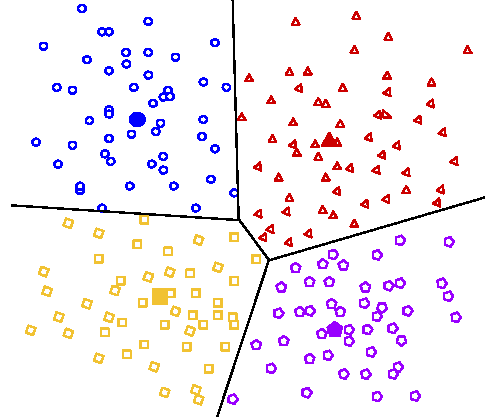
\includegraphics[width=5.0cm]{images/unsupervised/types/Clustering_CentroidBased.pdf}
					%\caption{Stripe Radar for Fraud Detection}
		\end{figure}
	%\end{block}

\end{frame}



\begin{frame}

	\frametitle{{\color{GradientDescentDiagramBlue}Centroid-based Clustering}: il K-means}

	\begin{scriptsize}
	\begin{block}{Come calcolare la media $\mu$ per un insieme di punti $\in \mathbb{R}^1$}
		\begin{figure}[!htbp]
			\centering
			\includegraphics<1>[width=0.7\linewidth]{images/unsupervised/kmeans/mean_r1.png}
			\includegraphics<2>[width=0.7\linewidth]{images/unsupervised/kmeans/mean_r1_mean.png}
					%\caption{Stripe Radar for Fraud Detection}
		\end{figure}
		
		\begin{itemize}
	        \item<1-> $\mu = \frac{2+3+7+8}{4} = 5$	       
	        \item<2-> $\mu = \frac{x_1 + x_2 + ... + x_N}{N} = \frac{1}{N}\sum_{i=1}^{N} x_i$
	    \end{itemize}

	\end{block}
	\end{scriptsize}
	
\end{frame}

\begin{frame}

	\frametitle{{\color{GradientDescentDiagramBlue}Centroid-based Clustering}: il K-means}

	\begin{scriptsize}
	\begin{block}{Come calcolare la media $\mu$ per un insieme di punti $\in \mathbb{R}^2$}
		\begin{figure}[!htbp]
			\centering
			\includegraphics<1>[width=0.56\linewidth]{images/unsupervised/kmeans/mean_r2.png}
			\includegraphics<2>[width=0.56\linewidth]{images/unsupervised/kmeans/mean_r2_mean.png}
					%\caption{Stripe Radar for Fraud Detection}
		\end{figure}
		
		\begin{align}
			\bar \mu = (\mu_1, \mu_2) &= \left(\frac{2+3+7+8}{4}, \frac{1+0+1+2}{4}\right) = (5,1)\nonumber \\
			\bar \mu = (\mu_1, \mu_2) &= \frac{1}{4} \left[(2,1) + (3,0) + (7,1) + (8,2)\right] \nonumber \\
			& = \frac{1}{4} (20, 4) \nonumber \\
			& = (5,1) \nonumber
		\end{align}
	\end{block}
	\end{scriptsize}
	
\end{frame}


\begin{frame}

	\frametitle{{\color{GradientDescentDiagramBlue}Centroid-based Clustering}: il K-means}
	
	\begin{scriptsize}
	\begin{block}{Come calcolare la media $\mu$ per un insieme di punti $\in \mathbb{R}^2$}
		\begin{figure}[!htbp]
			\centering
			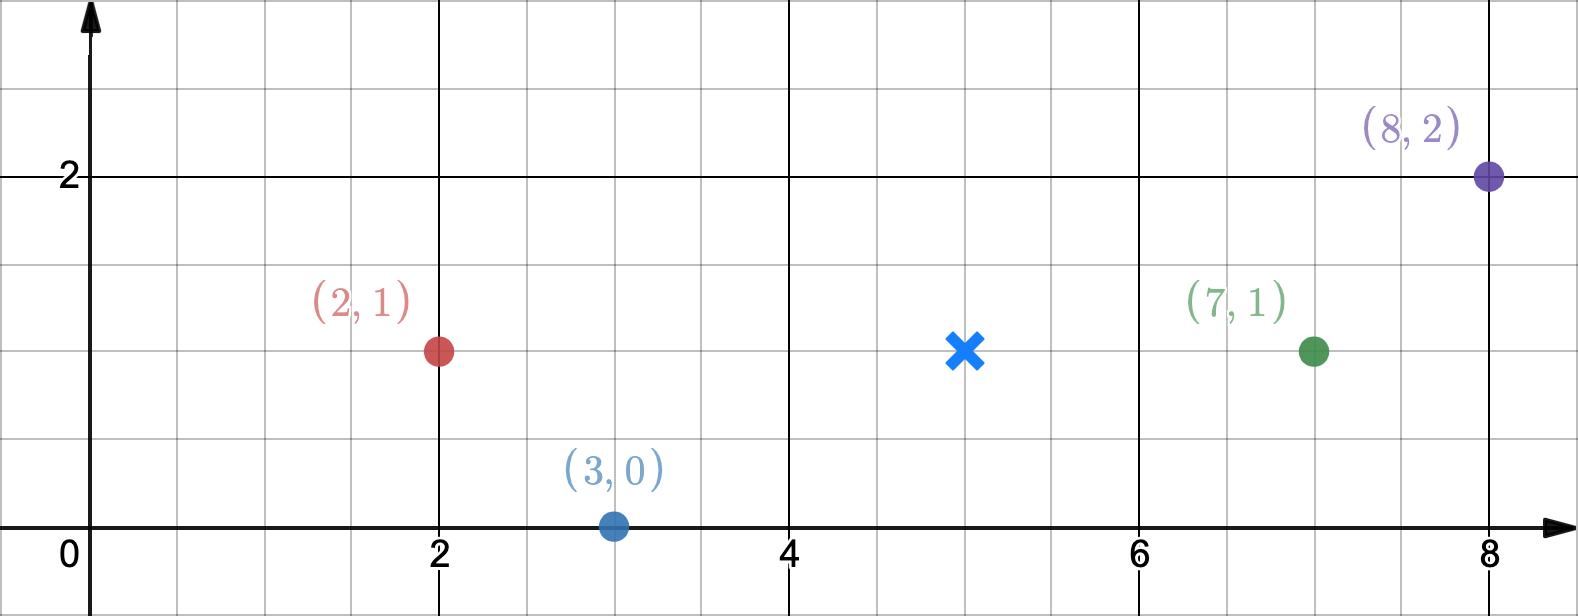
\includegraphics[width=0.5\linewidth]{images/unsupervised/kmeans/mean_r2_mean.png}
					%\caption{Stripe Radar for Fraud Detection}
		\end{figure}
		
		$$\bar \mu = (\mu_1, \mu_2) = \frac{1}{N} (\bar x_1 + \bar x_2 + ... + \bar x_N) = \frac{1}{N}\sum_{i=1}^{N} \bar x_i$$

	\end{block}
	
	\begin{block}{Come calcolare la media $\mu$ per un insieme di punti $\in \mathbb{R}^D$}
		$$\bar \mu = (\mu_1, \mu_2, ..., \mu_D) = \frac{1}{N} (\bar x_1 + \bar x_2 + ... + \bar x_N) = \frac{1}{N}\sum_{i=1}^{N} \bar x_i$$
	\end{block}
	\end{scriptsize}

\end{frame}




\begin{frame}

	\frametitle{{\color{GradientDescentDiagramBlue}Centroid-based Clustering}: il K-means}

	%\begin{block}{}
		Il clustering \textbf{K-means} è caratterizzato dai seguenti aspetti chiave:
		\begin{itemize}
			\item con il clustering K-means, il \textbf{numero K} di cluster deve essere specificato prima di iniziare il processo di clustering
			\item il clustering K-means \textbf{non è gerarchico}: il dataset è semplicemente partizionato in \textbf{K gruppi disgiunti}
			\ifthenelse{\boolean{highschool}}{}{
				\item K-means scala come $O(nk)$, dove $k$ è il numero di clusters e $n$ la dimensione del dataset
			}
		\end{itemize}
		
		\pause
		\vspace{2em}
		Definiamo la variabile binaria $r_{ik}$ che vale:
		\begin{itemize}
			\item 1: se l'$i$-esima osservazione $\in$ al cluster $k$
			\item 0: altrimenti
		\end{itemize}
		Ogni osservazione può essere assegnata ad un solo cluster, di conseguenza per ogni singola osservazione $i$ esisterà una e una sola $\hat{k}$ per il quale vale che  $r_{i\hat{k}}=1$.

	%\end{block}

\end{frame}



\begin{frame}

	\frametitle{{\color{GradientDescentDiagramBlue}Centroid-based Clustering}: il K-means}

	\begin{block}{K-means: algoritmo}
		\begin{enumerate}
			\item inizializza in modo casuale i valori delle variabili binarie $r_{ik}$ in modo che ogni punto sia assegnato casualmente ad un solo cluster 
			\item calcola la media di ogni cluster (cioè il centro del cluster):\\
				$\mu_k = \frac{\sum_{i=1}^{N}r_{ik}x_i}{\sum_{i=1}^{N}r_{ik}} =$ (la media delle osservazioni appartenti al cluster $k$)
			\item aggiorna i valori delle variabili binarie $r_{ik}$, in modo che ogni punto sia assegnato al centro del cluster più vicino
			\item se nessuna variabile viene aggiornata nel passaggio precedente, fermarsi, altrimenti tornare al passaggio 2
		\end{enumerate}
		\vspace{2mm}
		Una possibile inizializzazione alternativa prevede di fissare direttamente i centri dei clusters randomicamente (ad esempio scegliendo $k$ distinti punti random dal dataset) e poi procedere dal punto 3
	\end{block}

\end{frame}


\begin{frame}

	\frametitle{{\color{GradientDescentDiagramBlue}Centroid-based Clustering}: il K-means}

	\begin{block}{K-means: algoritmo}
		\begin{figure}[!htbp]
			\centering
			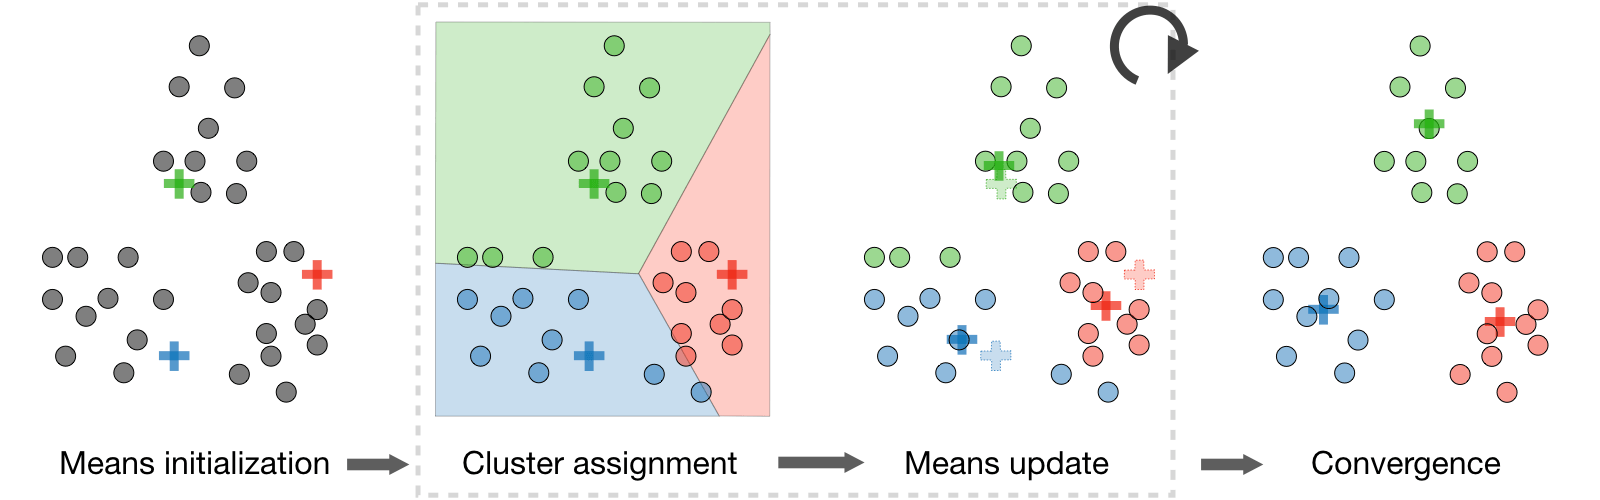
\includegraphics[width=1.0\linewidth]{images/unsupervised/kmeans/kmeans_algorithm.png}
					%\caption{Stripe Radar for Fraud Detection}
		\end{figure}
	\end{block}

\end{frame}


%\begin{frame}
%
%	\frametitle{{\color{GradientDescentDiagramBlue}Centroid-based Clustering}: il K-means}
%
%	\begin{block}{K-means: algoritmo\\Inizializzazione alternativa}
%		\begin{figure}[!htbp]
%			\centering
%			\includegraphics[width=5.75cm]{images/unsupervised/kmeans/kmeans_step_1.png}
%					%\caption{Stripe Radar for Fraud Detection}
%		\end{figure}
%	\end{block}
%
%\end{frame}
%
%
%\begin{frame}
%
%	\frametitle{{\color{GradientDescentDiagramBlue}Centroid-based Clustering}: il K-means}
%
%	\begin{block}{K-means: algoritmo\\Aggiorno gli $r_{ik}\text{ }$(punto 3)}
%		\begin{figure}[!htbp]
%			\centering
%			\includegraphics[width=5.75cm]{images/unsupervised/kmeans/kmeans_step_2.png}
%					%\caption{Stripe Radar for Fraud Detection}
%		\end{figure}
%	\end{block}
%
%\end{frame}
%
%
%\begin{frame}
%
%	\frametitle{{\color{GradientDescentDiagramBlue}Centroid-based Clustering}: il K-means}
%
%	\begin{block}{K-means: algoritmo\\La condizione di stop non è ancora rispettata quindi aggiorno i $\mu_k$ (punto 2)}
%		\begin{figure}[!htbp]
%			\centering
%			\includegraphics[width=5.75cm]{images/unsupervised/kmeans/kmeans_step_3.png}
%					%\caption{Stripe Radar for Fraud Detection}
%		\end{figure}
%	\end{block}
%
%\end{frame}
%
%
%\begin{frame}
%
%	\frametitle{{\color{GradientDescentDiagramBlue}Centroid-based Clustering}: il K-means}
%
%	\begin{block}{K-means: algoritmo\\Aggiorno gli $r_{ik}\text{ }$(punto 3)}
%		\begin{figure}[!htbp]
%			\centering
%			\includegraphics[width=5.75cm]{images/unsupervised/kmeans/kmeans_step_4.png}
%					%\caption{Stripe Radar for Fraud Detection}
%		\end{figure}
%	\end{block}
%
%\end{frame}


\begin{frame}

	\frametitle{{\color{GradientDescentDiagramBlue}Centroid-based Clustering}: il K-means}

%	\begin{block}{K-means: algoritmo}
		\centering
		\animategraphics[controls={play, step, stop}, height=7cm]{20.0}{images/unsupervised/kmeans/k_means_1/k_means_1-}{0}{242}
%	\end{block}

\end{frame}


\begin{frame}

	\frametitle{{\color{GradientDescentDiagramBlue}Centroid-based Clustering}: il K-means}

%	\begin{block}{K-means: algoritmo}
		\centering
		\animategraphics[controls={play, step, stop}, height=7cm]{3.0}{images/unsupervised/kmeans/k_means_2/k_means_2-}{0}{14}
%	\end{block}

\end{frame}


\begin{frame}

	\frametitle{{\color{GradientDescentDiagramBlue}Centroid-based Clustering}: il K-means}

%	\begin{block}{K-means: algoritmo}
		\centering
		\animategraphics[controls={play, step, stop}, height=7cm]{3.0}{images/unsupervised/kmeans/k_means_3/k_means_3-}{0}{12}
%	\end{block}

\end{frame}


\begin{frame}

	\frametitle{{\color{GradientDescentDiagramBlue}Centroid-based Clustering}: il K-means}

	\begin{block}{}
		Per altri esempi interattivi:\\
		\begin{itemize}
			\item \underline{\href{https://stanford.edu/class/engr108/visualizations/kmeans/kmeans.html}{Esempio 1}}
			\item \underline{\href{http://alekseynp.com/viz/k-means.html}{Esempio 2}}
		\end{itemize}
	\end{block}

\end{frame}


\ifthenelse{\boolean{highschool}}{}{
	\begin{frame}
	
		\frametitle{{\color{GradientDescentDiagramBlue}Centroid-based Clustering}: il K-means}
	
		\begin{block}{K-means: dimostrazione matematica parte 1}
			Ricordiamo l'espressione di:
			\begin{empheq}[box=\fcolorbox{blue!40!black!60}{yellow!10}]{align*}
				\mathbf{J} = \frac{1}{N} \sum_{i=1}^{N}\sum_{k=1}^{K}r_{ik} \Vert x_i-\mu_k\Vert^2
			\end{empheq}
	
			Dati $N$ esempi assegnati a $K$ cluster, minimizziamo la somma delle distanze degli esempi rispetto ai loro centroidi. Dove:
			\begin{itemize}
				\item $r_{ik}=1$ quando l'$i$-esimo esempio è assegnato al $k$-esimo cluster, $=0$ altrimenti
				\item $\mu_k$ è il centroide del $k$-esimo cluster
			\end{itemize}
		\end{block}
	
	\end{frame}
	
	
	\begin{frame}
	
		\frametitle{{\color{GradientDescentDiagramBlue}Centroid-based Clustering}: il K-means}
	
		\begin{block}{K-means: dimostrazione matematica parte 2}
	
			Vogliamo quindi minimizzare la seguente espressione:
			$$\underset{r,\mu}{min}\sum_{i=1}^{N}\sum_{k=1}^{K}r_{ik} \Vert x_i-\mu_k\Vert^2$$
			dove:
			$$r_{ik} \in \{0,1\}\quad\forall i,k$$
			e
			$$\sum^{K}_{k=1}r_{ik}=1\quad\forall i$$
	
			Per minimizzare l'espressione rispetto al cluster con centroide $\mu_k$, deriviamo rispetto a $\mu_k$ e la uguagliamo a 0.
		\end{block}
	
	\end{frame}
	
	
	\begin{frame}
	
		\frametitle{{\color{GradientDescentDiagramBlue}Centroid-based Clustering}: il K-means}
	
		\begin{block}{K-means: dimostrazione matematica parte 3}
			
			\begin{center}
				$f(\mu) = \sum^{N}_{i=1} \sum_{k=1}^{K} r_{ik} ||x_i - \mu_k||^2$ \newlinedouble %\hline
				$\frac{\partial f}{\partial \mu_k} = 2 \sum_{i=1}^{N} r_{ik}(x_i - \mu_k) = 0$  \\~\\ $\pmb{\Downarrow}$ \\~\\
				 %\hline
				$\quad \sum_{i=1}^{N} r_{ik}\mu_{k} = \sum_{i=1}^{N} r_{ik}x_{i}$ \newlinedouble %\hline
				$\mu_k \sum_{i=1}^{N} r_{ik} = \sum_{i=1}^{N} r_{ik} x_i$ \newlinedouble %\hline
				$\mu_k = \frac{\sum_{i=1}^{N} r_{ik} x_i}{\sum_{i=1}^{N} r_{ik}}$	
			\end{center}
	
		\end{block}
	
	\end{frame}
	
	
	\begin{frame}
	
		\frametitle{{\color{GradientDescentDiagramBlue}Centroid-based Clustering}: il K-means}
	
		\begin{block}{K-means: dimostrazione matematica parte 4}
	
	%		\begin{scriptsize}
				\begin{gather*}
					 \mu_k = \frac{\sum_{i=1}^{N} r_{ik} x_i}{\sum_{i=1}^{N} r_{ik}}
				\end{gather*}
	%		\end{scriptsize}
	
			\begin{itemize}
				\item il \textbf{numeratore} è la somma di tutti i  punti (vettori) appartenti al cluster
				\item il \textbf{denominatore} è il numero di esempi nel cluster
				\item pertanto, il centroide del cluster $\mu_k$ è la media delle posizioni dei punti appartenenti al cluster
				\item quindi in estrema sintesi: per minimizzare $J$ è sufficiente aggiornare il $\mu_k$ del cluster sommando i vari vettori (punti) del cluster e dividere per il numero di elementi del cluster (media di tutti i punti nel cluster)
			\end{itemize}
	
		\end{block}
	
	\end{frame}
}


\begin{frame}

	\frametitle{{\color{GradientDescentDiagramBlue}Centroid-based Clustering}: il K-means}

	\begin{block}{K-means: svantaggi}
		\begin{itemize}
			\item uno svantaggio del clustering k-means è che non è garantito che converga sempre allo stesso clustering
				\begin{itemize}
					\item[--] l'esecuzione della procedura più volte può produrre cluster diversi: a seconda dell'inizializzazione randomica l'algoritmo può convergere a minimi (locali) diversi
				\end{itemize}
			\item un altro svantaggio è che l'uso della distanza euclidea determina cluster sferici
		\end{itemize}
	\end{block}

\end{frame}


\begin{frame}

	\frametitle{{\color{GradientDescentDiagramBlue}Centroid-based Clustering}: il K-means}

	\begin{block}{K-means: minimi locali diversi parte 1}
		\begin{itemize}
			\item Considera il seguente dataset composto da punti 2D appartenenti a 2 classi distinte
			\item ogni classe è caratterizzata da una distribuzione gaussiana (parzialmente sovrapposta)
		\end{itemize}

		\begin{figure}[!htbp]
			\centering
			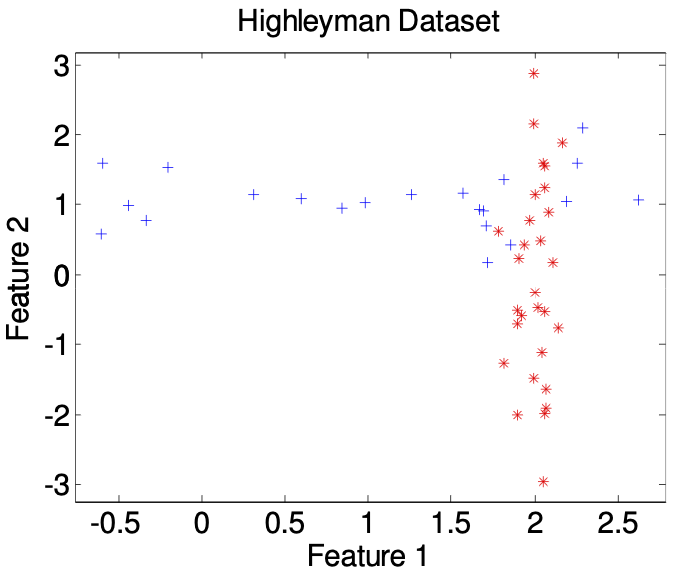
\includegraphics[width=4.50cm]{images/unsupervised/kmeans/highley_gt.png}
					%\caption{Stripe Radar for Fraud Detection}
		\end{figure}
	\end{block}

\end{frame}


\begin{frame}

	\frametitle{{\color{GradientDescentDiagramBlue}Centroid-based Clustering}: il K-means}

	\begin{block}{K-means: minimi locali diversi parte 2}
		Risultato usando K-means con $K=2$
		\begin{columns}
			\column{0.5\linewidth}
			\begin{figure}[!htbp]
				\centering
				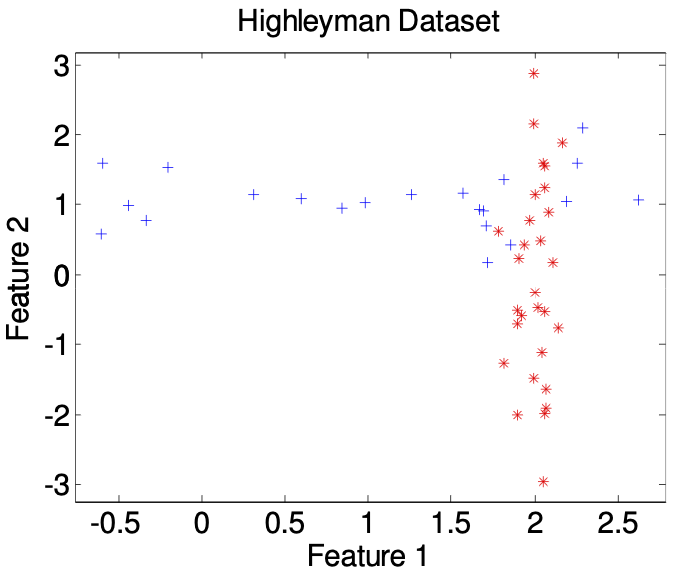
\includegraphics[angle=0,width=1\linewidth]{images/unsupervised/kmeans/highley_gt.png}
%				\caption{Single-Link Good K}
				%\label{Enel_HistFit_Normal}
			\end{figure}

			\column{0.5\linewidth}
			\begin{figure}[!htbp]
				\centering
				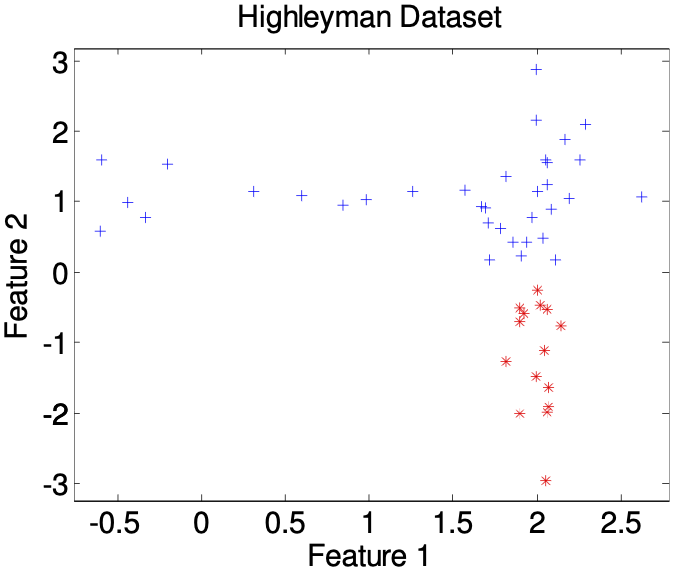
\includegraphics[angle=0,width=1\linewidth]{images/unsupervised/kmeans/highley_2k.png}
%				\caption{Single-Link Dendogram Good K}
				%\label{Enel_QQ_Plot_Normal}
			\end{figure}

		\end{columns}
	\end{block}

\end{frame}



\begin{frame}

	\frametitle{{\color{GradientDescentDiagramBlue}Centroid-based Clustering}: il K-means}

	\begin{block}{K-means: minimi locali diversi parte 3}
		Risultato 1 usando K-means con $K=3$
		\begin{columns}
			\column{0.5\linewidth}
			\begin{figure}[!htbp]
				\centering
				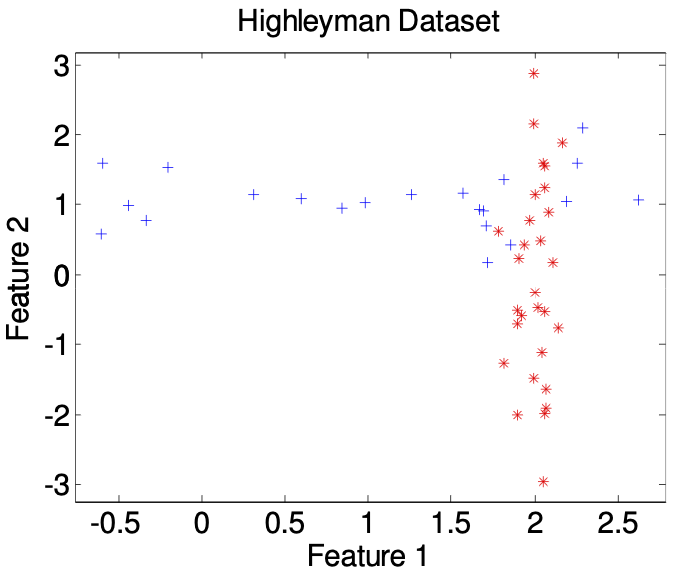
\includegraphics[angle=0,width=1\linewidth]{images/unsupervised/kmeans/highley_gt.png}
%				\caption{Single-Link Good K}
				%\label{Enel_HistFit_Normal}
			\end{figure}

			\column{0.5\linewidth}
			\begin{figure}[!htbp]
				\centering
				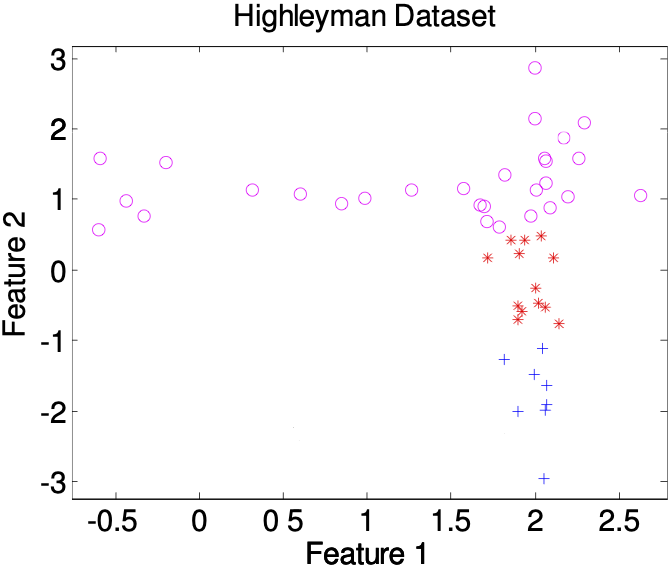
\includegraphics[angle=0,width=1\linewidth]{images/unsupervised/kmeans/highley_3k_1.png}
%				\caption{Single-Link Dendogram Good K}
				%\label{Enel_QQ_Plot_Normal}
			\end{figure}

		\end{columns}
	\end{block}

\end{frame}


\begin{frame}

	\frametitle{{\color{GradientDescentDiagramBlue}Centroid-based Clustering}: il K-means}

	\begin{block}{K-means: minimi locali diversi parte 4}
		Risultato 2 usando K-means con $K=3$
		\begin{columns}
			\column{0.5\linewidth}
			\begin{figure}[!htbp]
				\centering
				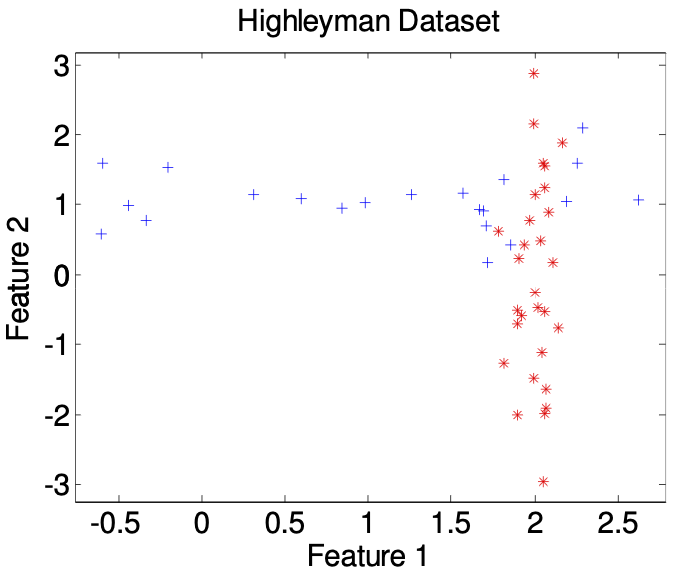
\includegraphics[angle=0,width=1\linewidth]{images/unsupervised/kmeans/highley_gt.png}
%				\caption{Single-Link Good K}
				%\label{Enel_HistFit_Normal}
			\end{figure}

			\column{0.5\linewidth}
			\begin{figure}[!htbp]
				\centering
				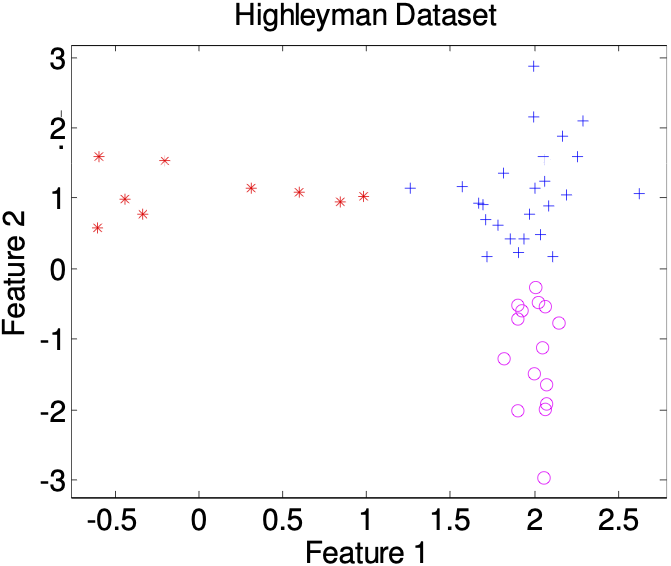
\includegraphics[angle=0,width=1\linewidth]{images/unsupervised/kmeans/highley_3k_2.png}
%				\caption{Single-Link Dendogram Good K}
				%\label{Enel_QQ_Plot_Normal}
			\end{figure}

		\end{columns}
	\end{block}

\end{frame}


\begin{frame}

	\frametitle{{\color{GradientDescentDiagramBlue}Centroid-based Clustering}: considerazioni}

	%\begin{block}{K-means: considerazioni}

		\begin{itemize}
			\item La procedura iterativa K-means cerca di spostare i centri del cluster in modo da farli corrispondere a posizioni nello spazio delle features in cui si concentrano molti punti
				\begin{itemize}
					\item[--] idealmente, i centri dei cluster dovrebbero essere posizionati in corrispondenza dei \textbf{picchi della densità} di distribuzione dei dati nello spazio delle features
				\end{itemize}
			\item Un risultato dell'utilizzo della distanza euclidea per valutare la vicinanza di un punto dati al centro del suo cluster è che la forma di ciascun cluster rappresenta una cella Voronoi
				\begin{itemize}
					\item[--] l'insieme di tutti i cluster determina una \textbf{tassellazione Voronoi} del spazio delle caratteristiche
				\end{itemize}
		\end{itemize}

		\begin{figure}[!htbp]
				\centering
				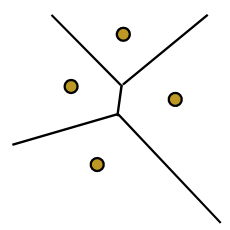
\includegraphics[angle=0,width=0.18\linewidth]{images/unsupervised/kmeans/kmeans_voronoi.png}
%				\caption{Single-Link Dendogram Good K}
				%\label{Enel_QQ_Plot_Normal}
			\end{figure}
	%\end{block}

\end{frame}


\begin{frame}

	\frametitle{{\color{GradientDescentDiagramBlue}Centroid-based Clustering}: segmentazione con il K-means}

%	\begin{block}{K-means: considerazioni}
		\begin{figure}[!htbp]
			\centering
			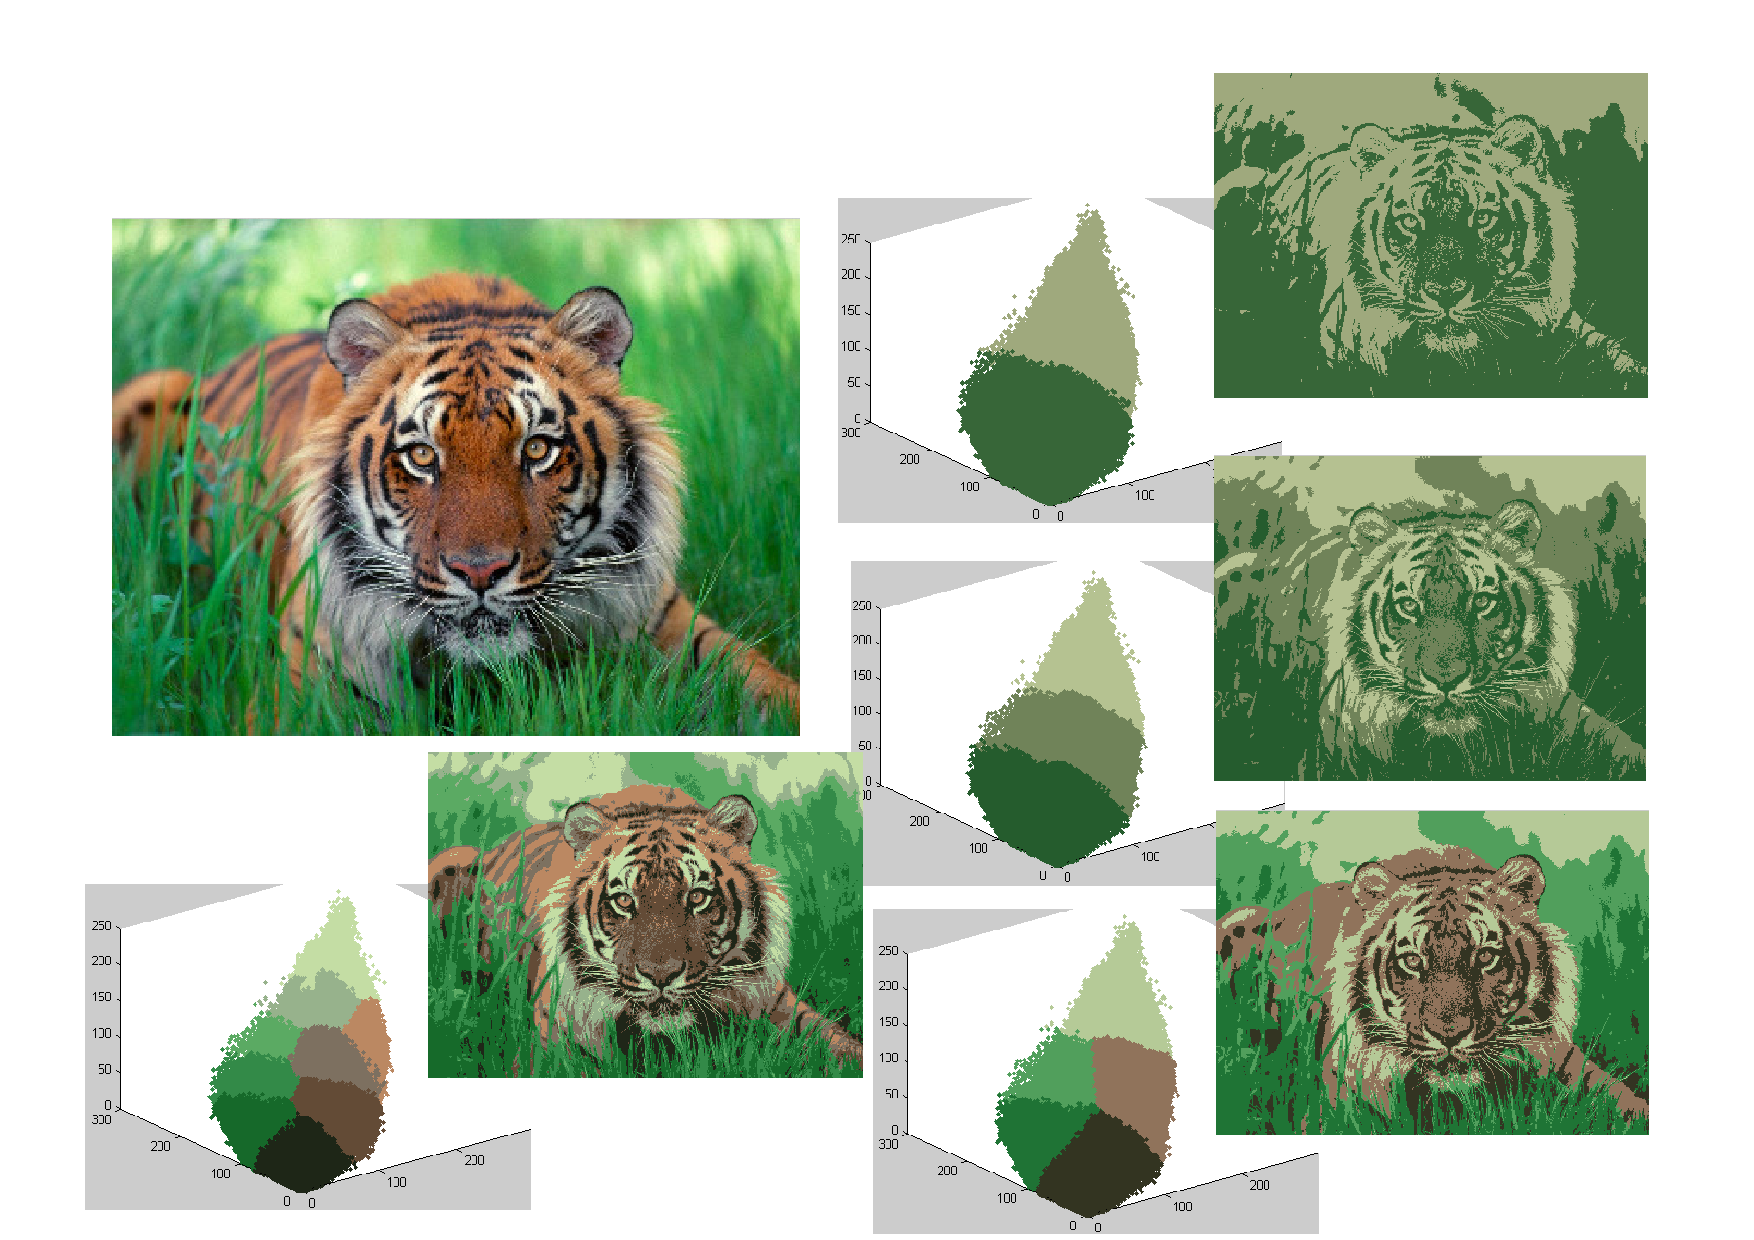
\includegraphics[angle=0,width=0.8\linewidth]{images/unsupervised/kmeans/kmeans_lion.pdf}
%				\caption{Single-Link Dendogram Good K}
			%\label{Enel_QQ_Plot_Normal}
		\end{figure}
%	\end{block}

\end{frame}


\begin{frame}

	\frametitle{{\color{GradientDescentDiagramBlue}Centroid-based Clustering}: segmentazione con il K-means}

%	\begin{block}{K-means: considerazioni}
		\begin{figure}[!htbp]
				\centering
				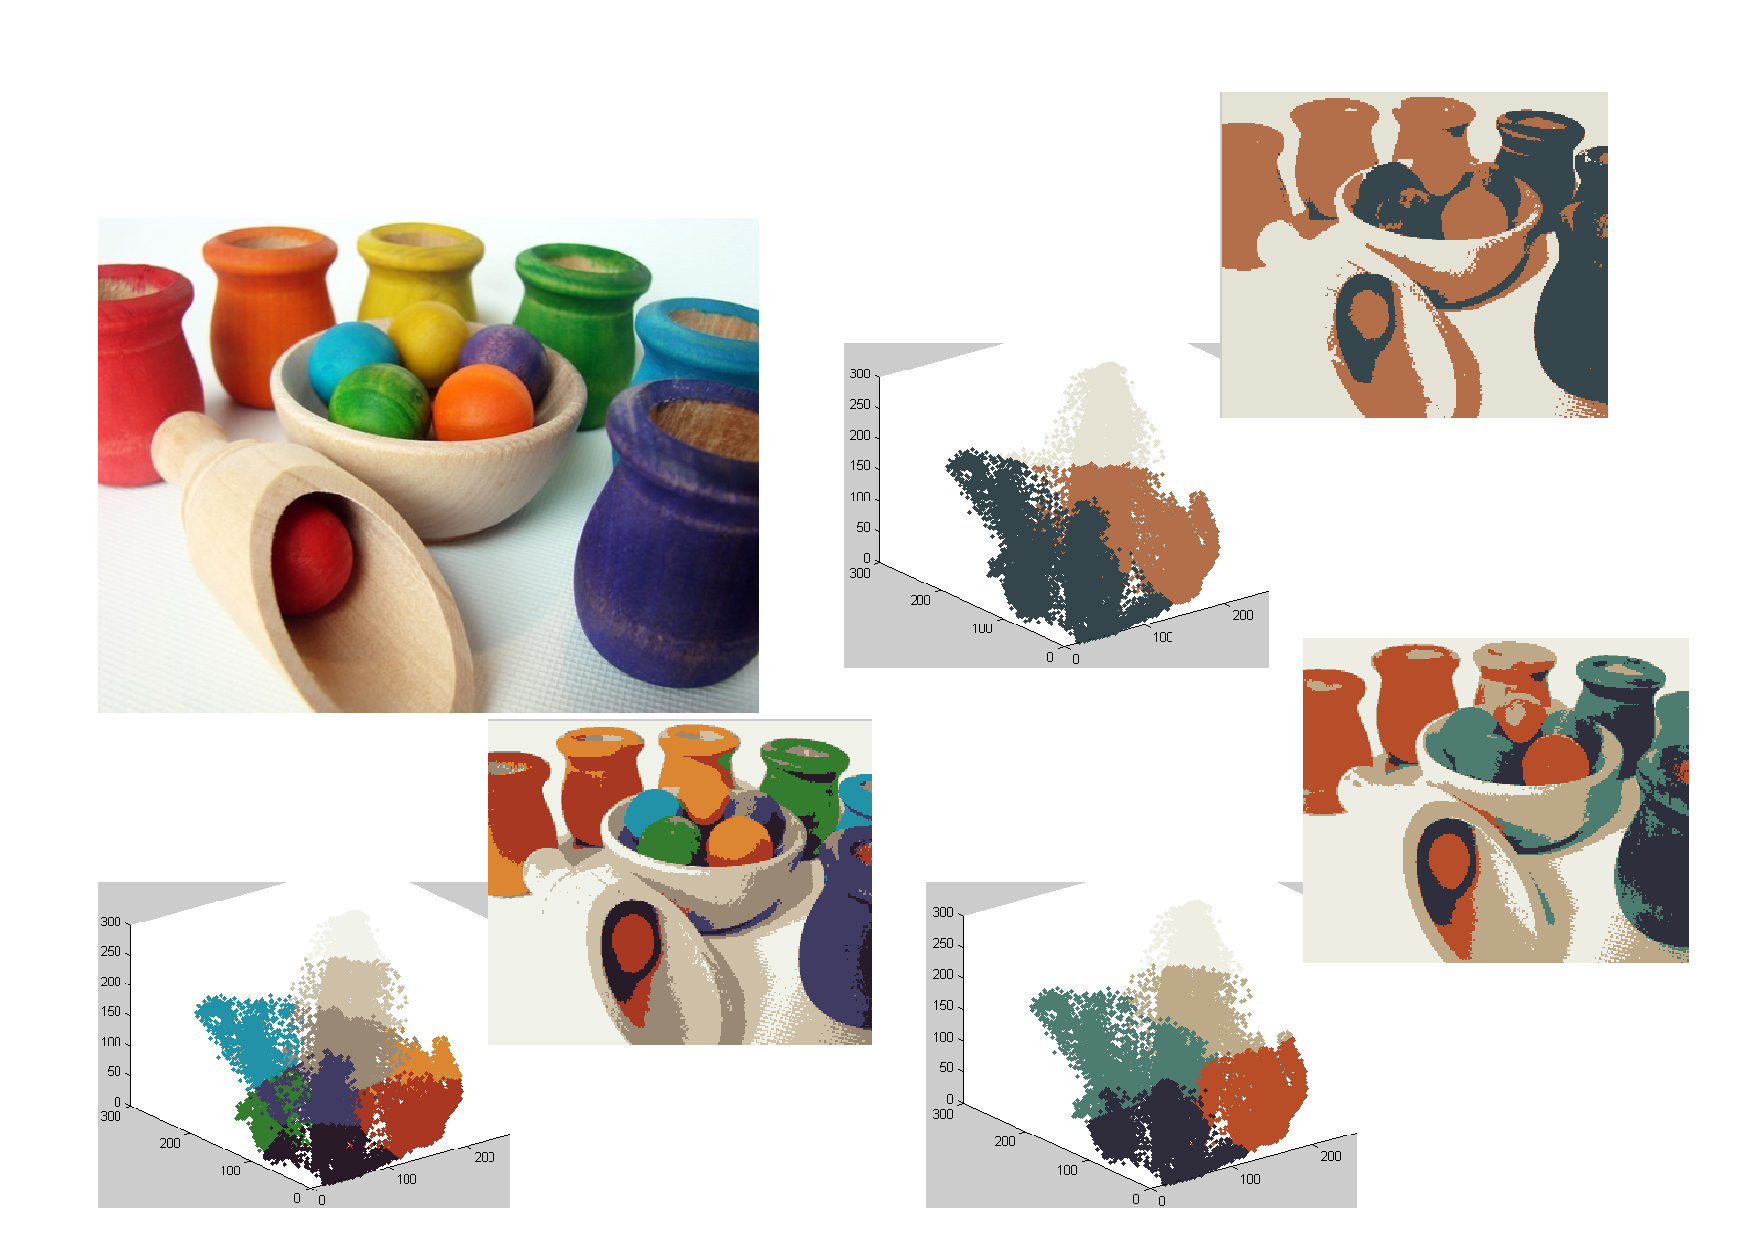
\includegraphics[angle=0,width=0.85\linewidth]{images/unsupervised/kmeans/kmeans_pots.pdf}
%				\caption{Single-Link Dendogram Good K}
				%\label{Enel_QQ_Plot_Normal}
			\end{figure}
%	\end{block}

\end{frame}


\subsubsection[Hierarchical (AGNES e DIANA)]{Hierarchical \textit{(AGNES e DIANA)}}
\begin{frame}

	\frametitle{{\color{GradientDescentDiagramGreen}Hierarchical Clustering}, in sintesi}

	%\begin{block}{}
		Il clustering gerarchico crea un albero di clusters.\\
		È una metodologia di clustering che cerca di costruire una gerarchia di cluster, rappresentata con un albero che prende il nome di \emph{dendogramma}.\newlinedouble
		%Mira a creare una sorta di tassonomia al variare del numero di clusters $K$.\\ %  da $1$ a $N$ dove $N$ è il numero di osservazioni del dataset.
		È possibile decidere un numero $K$ qualsiasi di clusters per il nostro specifico problema tagliando l'albero costruito con tale procedura al giusto livello.
		\begin{figure}[!htbp]
			\centering
			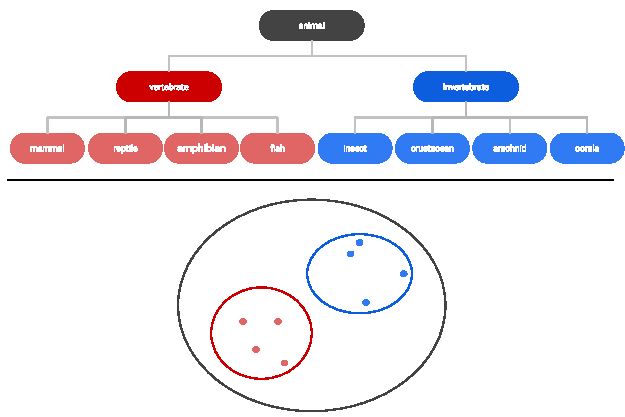
\includegraphics[width=7.0cm]{images/unsupervised/types/Clustering_Hierarchical.pdf}
					%\caption{Stripe Radar for Fraud Detection}
		\end{figure}
	%\end{block}

\end{frame}


\begin{frame}

	\frametitle{{\color{GradientDescentDiagramGreen}Hierarchical Clustering}}

%	\begin{block}{Idea di base}
		Il clustering gerarchico può essere suddiviso in due tipologie principali:
		\begin{itemize}
			\item \textbf{clustering gerarchico agglomerativo}: è noto anche come \textbf{AGNES} (Agglomerative Nesting, bottom-up). Cioè, ogni oggetto viene inizialmente considerato come un cluster a elemento singolo (foglia). Ad ogni passaggio dell'algoritmo, i due cluster più simili vengono combinati in un nuovo cluster più grande (nodi). Questa procedura viene ripetuta finché tutti i punti non sono membri di un unico grande cluster (radice). Il risultato è un albero che può essere tracciato come un dendrogramma.
			\item \textbf{clustering gerarchico divisivo}: è noto anche come \textbf{DIANA} (Divise Analysis, top-down). L'algoritmo procede in ordine inverso rispetto all'AGNES. Inizia con la radice, in cui tutti gli oggetti sono inclusi in un singolo cluster. In ogni fase dell'iterazione, il cluster più eterogeneo viene diviso in due. Il processo viene iterato fino a quando tutti gli oggetti si trovano nel loro proprio cluster.
		\end{itemize}
%	\end{block}
\end{frame}


\begin{frame}

	\frametitle{{\color{GradientDescentDiagramGreen}Hierarchical Clustering}}

%	\begin{block}{Idea di base}
		\ifthenelse{\boolean{highschool}}{}{Si noti che il clustering agglomerativo è utile per identificare piccoli cluster. Il clustering divisivo è utile per identificare cluster di grandi dimensioni.}
		\begin{figure}[!htbp]
			\centering
			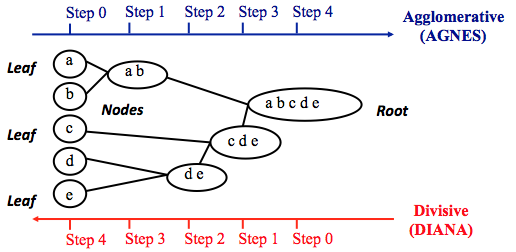
\includegraphics[width=12.0cm]{images/unsupervised/hierarchical/hierarchical-clustering-agnes-diana.png}
					%\caption{Stripe Radar for Fraud Detection}
		\end{figure}

%	\end{block}
\end{frame}



\begin{frame}

	\frametitle{{\color{GradientDescentDiagramGreen}Hierarchical Clustering}}

	\begin{block}{Clustering gerarchico agglomerativo: idea di base}
		\begin{itemize}
			\item agglomerare ricorsivamente i punti in cluster combinando i punti e i cluster più vicini per ottenere cluster più grandi fino a quando tutti i punti vengono raccolti in un solo cluster
		\end{itemize}
		Il processo ricorsivo definisce una gerarchia che rende esplicita la struttura del set di dati in termini di cluster di grandi dimensioni e sub-clusters.
		\newlinedouble
		Il clustering gerarchico richiede la specifica di come calcolare la distanza tra:
		\begin{itemize}
			\item due punti (Manhattan, Euclidean, cosine ...)
			\item un punto e un cluster (...)
			\item due cluster (...)
		\end{itemize}
	\end{block}

\end{frame}


\begin{frame}

	\frametitle{{\color{GradientDescentDiagramGreen}Hierarchical Clustering}}

	\begin{block}{Clustering gerarchico agglomerativo: algoritmo}
		\begin{enumerate}
			\item all'inizio, ogni punto definisce un nuovo cluster, risultando in N cluster ciascuno contenente un solo punto. Le distanze tra tutte le coppie di cluster vengono calcolate e memorizzate in una matrice $A_{NN}$
			\item trovare la coppia di cluster più vicina e unirli in un unico cluster. Calcola e memorizza la distanza tra il nuovo cluster e tutti gli altri (ovvero, aggiorna $A_{NN}$)
			\item ripeti il passaggio 2 fino a quando tutti i punti sono raggruppati in un unico cluster composto da $N$ punti
		\end{enumerate}
	\end{block}

\end{frame}


\begin{frame}

	\frametitle{{\color{GradientDescentDiagramGreen}Hierarchical Clustering}}

	\begin{block}{Metriche di dissimilarità più utilizzate: (indicate successivamente con $\bigstar$)}

		\begin{itemize}
			\item \textbf{Euclidean distance}:\\
				\makebox[\textwidth]{$d_{euc}(x,y) = \sqrt{\sum^n_{i=1}(x_i - y_i)^2}$}
			\item \textbf{Manhattan distance}:\\
				\makebox[\textwidth]{$d_{man}(x,y) = \sum^n_{i=1}|(x_i - y_i)|$}
			\item \textbf{Pearson correlation distance}:\\
				\makebox[\textwidth]{$d_{cor}(x, y) = 1 - \frac{\sum^n_{i=1}(x_i-\bar x)(y_i - \bar y)}{\sqrt{\sum^n_{i=1}(x_i-\bar x)^2\sum^n_{i=1}(y_i - \bar y)^2}}$}
			\ifthenelse{\boolean{highschool}}{
			\item \textbf{\underline{\href{https://uc-r.github.io/kmeans_clustering\#distance}{Altre...}}}}{
			\item \textbf{Spearman correlation distance}:\\
				\makebox[\textwidth]{$d_{spear}(x, y) = 1 - \frac{\sum^n_{i=1}(x^\prime_i-\bar x^\prime)(y^\prime_i - \bar y^\prime)}{\sqrt{\sum^n_{i=1}(x^\prime_i-\bar x^\prime)^2\sum^n_{i=1}(y^\prime_i - \bar y^\prime)^2}} \rightarrow$ \underline{\href{https://uc-r.github.io/kmeans_clustering\#distance}{link per dettagli}}}
			\item \textbf{Kendall correlation distance}:\\
				\makebox[\textwidth]{$d_{kend}(x,y) = 1 - \frac{n_c - n_d}{\frac{1}{2}n(n - 1)} \rightarrow$ \underline{\href{https://uc-r.github.io/kmeans_clustering\#distance}{link per dettagli}}}
			}
		\end{itemize}


	\end{block}

\end{frame}


\begin{frame}

	\frametitle{{\color{GradientDescentDiagramGreen}Hierarchical Clustering}}

	\begin{block}{La distanza tra due clusters $C_i$ e $C_j$ è calcolata come:}
		\begin{itemize}
			\item nel \textbf{single-link} clustering:\\
				come la \textit{minima distanza} tra un punto di $C_i$ e un punto di $C_j$\\
				\makebox[\textwidth]{$d_{SL}(C_i, C_j) = \underset{x \in C_i, y \in C_j}{min} d_{\bigstar}(x, y)$}
				\vspace{0.5mm}
			\item nel \textbf{average-link} clustering:\\
				come la \textit{distanza media} tra un punto di $C_i$ e un punto di $C_j$\\
				\makebox[\textwidth]{$d_{AVG}(C_i, C_j) = \underset{x \in C_i, y \in C_j}{avg} d_{\bigstar}(x, y)$}
				\vspace{0.5mm}
			\item nel \textbf{complete-link} clustering:\\
				come la \textit{massima distanza} tra un punto di $C_i$ e un punto di $C_j$\\
				\makebox[\textwidth]{$d_{CL}(C_i, C_j) = \underset{x \in C_i, y \in C_j}{max} d_{\bigstar}(x, y)$}
		\end{itemize}
		Esistono altre metriche di distanze tra clusters, vedi \underline{\href{https://uc-r.github.io/hc_clustering}{link per dettagli}}.
	\end{block}

\end{frame}


\begin{frame}

	\frametitle{{\color{GradientDescentDiagramGreen}Hierarchical Clustering}}

	%\begin{block}{}
		\begin{itemize}
			\item si noti che la distanza tra due cluster può essere misurata in modi diversi
			\item indipendentemente da ciò, ad ogni passaggio i due cluster più vicini vengono aggregati
			\item tipicamente, prima di iniziare il processo di clusterizzazione, i valori delle features vengono scalati in modo da avere media zero e deviazione standard unitaria
		\end{itemize}

	%\end{block}

\end{frame}


\begin{frame}

	\frametitle{{\color{GradientDescentDiagramGreen}Hierarchical Clustering}: Euclidean + Single-Link}

	%\begin{block}{}

		\begin{figure}[!htbp]
			\centering
			
			\includegraphics<1>[width=0.70\linewidth, height=7.2cm]{images/unsupervised/hierarchical/hierarchical_single_link_1.png}
			\includegraphics<2>[width=0.70\linewidth, height=7.2cm]{images/unsupervised/hierarchical/hierarchical_single_link_2.png}
			\includegraphics<3>[width=0.70\linewidth, height=7.2cm]{images/unsupervised/hierarchical/hierarchical_single_link_3.png}
			\includegraphics<4>[width=0.70\linewidth, height=7.2cm]{images/unsupervised/hierarchical/hierarchical_single_link_4.png}
			\includegraphics<5>[width=0.70\linewidth, height=7.2cm]{images/unsupervised/hierarchical/hierarchical_single_link_5.png}
			\includegraphics<6>[width=0.70\linewidth, height=7.2cm]{images/unsupervised/hierarchical/hierarchical_single_link_6.png}
			
			%\caption{Single-Link}
			%\label{Enel_HistFit_Normal}
		\end{figure}

	%\end{block}

\end{frame}


\begin{frame}

	\frametitle{{\color{GradientDescentDiagramGreen}Hierarchical Clustering}: Euclidean + Complete-Link}

	%\begin{block}{}

		\begin{figure}[!htbp]
			\centering
			
			\includegraphics<1>[width=0.70\linewidth, height=7.2cm]{images/unsupervised/hierarchical/hierarchical_complete_link_1.png}
			\includegraphics<2>[width=0.70\linewidth, height=7.2cm]{images/unsupervised/hierarchical/hierarchical_complete_link_2.png}
			\includegraphics<3>[width=0.70\linewidth, height=7.2cm]{images/unsupervised/hierarchical/hierarchical_complete_link_3.png}
			\includegraphics<4>[width=0.70\linewidth, height=7.2cm]{images/unsupervised/hierarchical/hierarchical_complete_link_4.png}
			\includegraphics<5>[width=0.70\linewidth, height=7.2cm]{images/unsupervised/hierarchical/hierarchical_complete_link_5.png}
			\includegraphics<6>[width=0.70\linewidth, height=7.2cm]{images/unsupervised/hierarchical/hierarchical_complete_link_6.png}
			
			%\caption{Complete-Link}
			%\label{Enel_QQ_Plot_Normal}
		\end{figure}

	%\end{block}

\end{frame}


\begin{frame}

	\frametitle{{\color{GradientDescentDiagramGreen}Hierarchical Clustering}}

	%\begin{block}{}

		\begin{columns}

			\column{0.5\linewidth}
			\begin{figure}[!htbp]
				\centering
				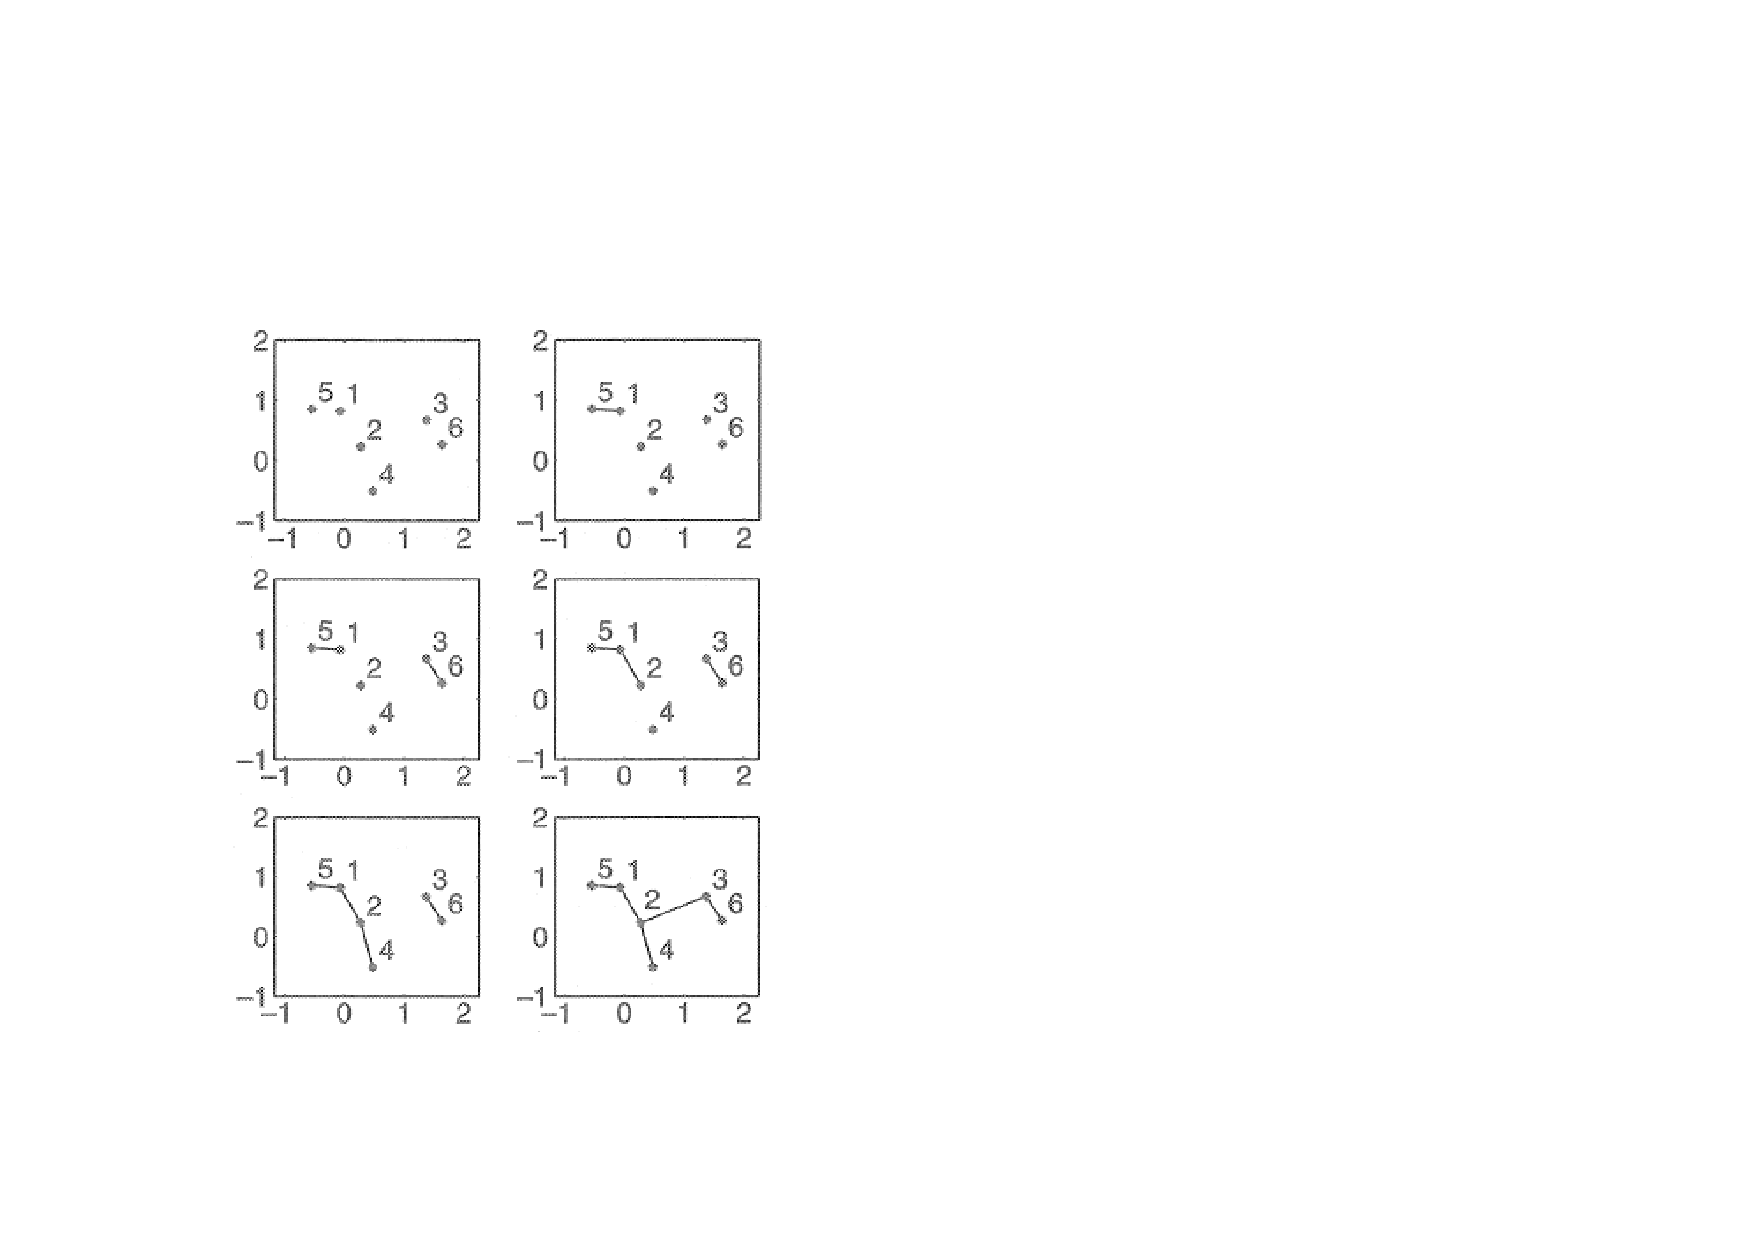
\includegraphics[angle=0,width=0.75\linewidth]{images/unsupervised/hierarchical/hierarchical_single_link.pdf}
				\caption{Euclidean + Single-Link}
				%\label{Enel_HistFit_Normal}
			\end{figure}

			\column{0.5\linewidth}
			\begin{figure}[!htbp]
				\centering
				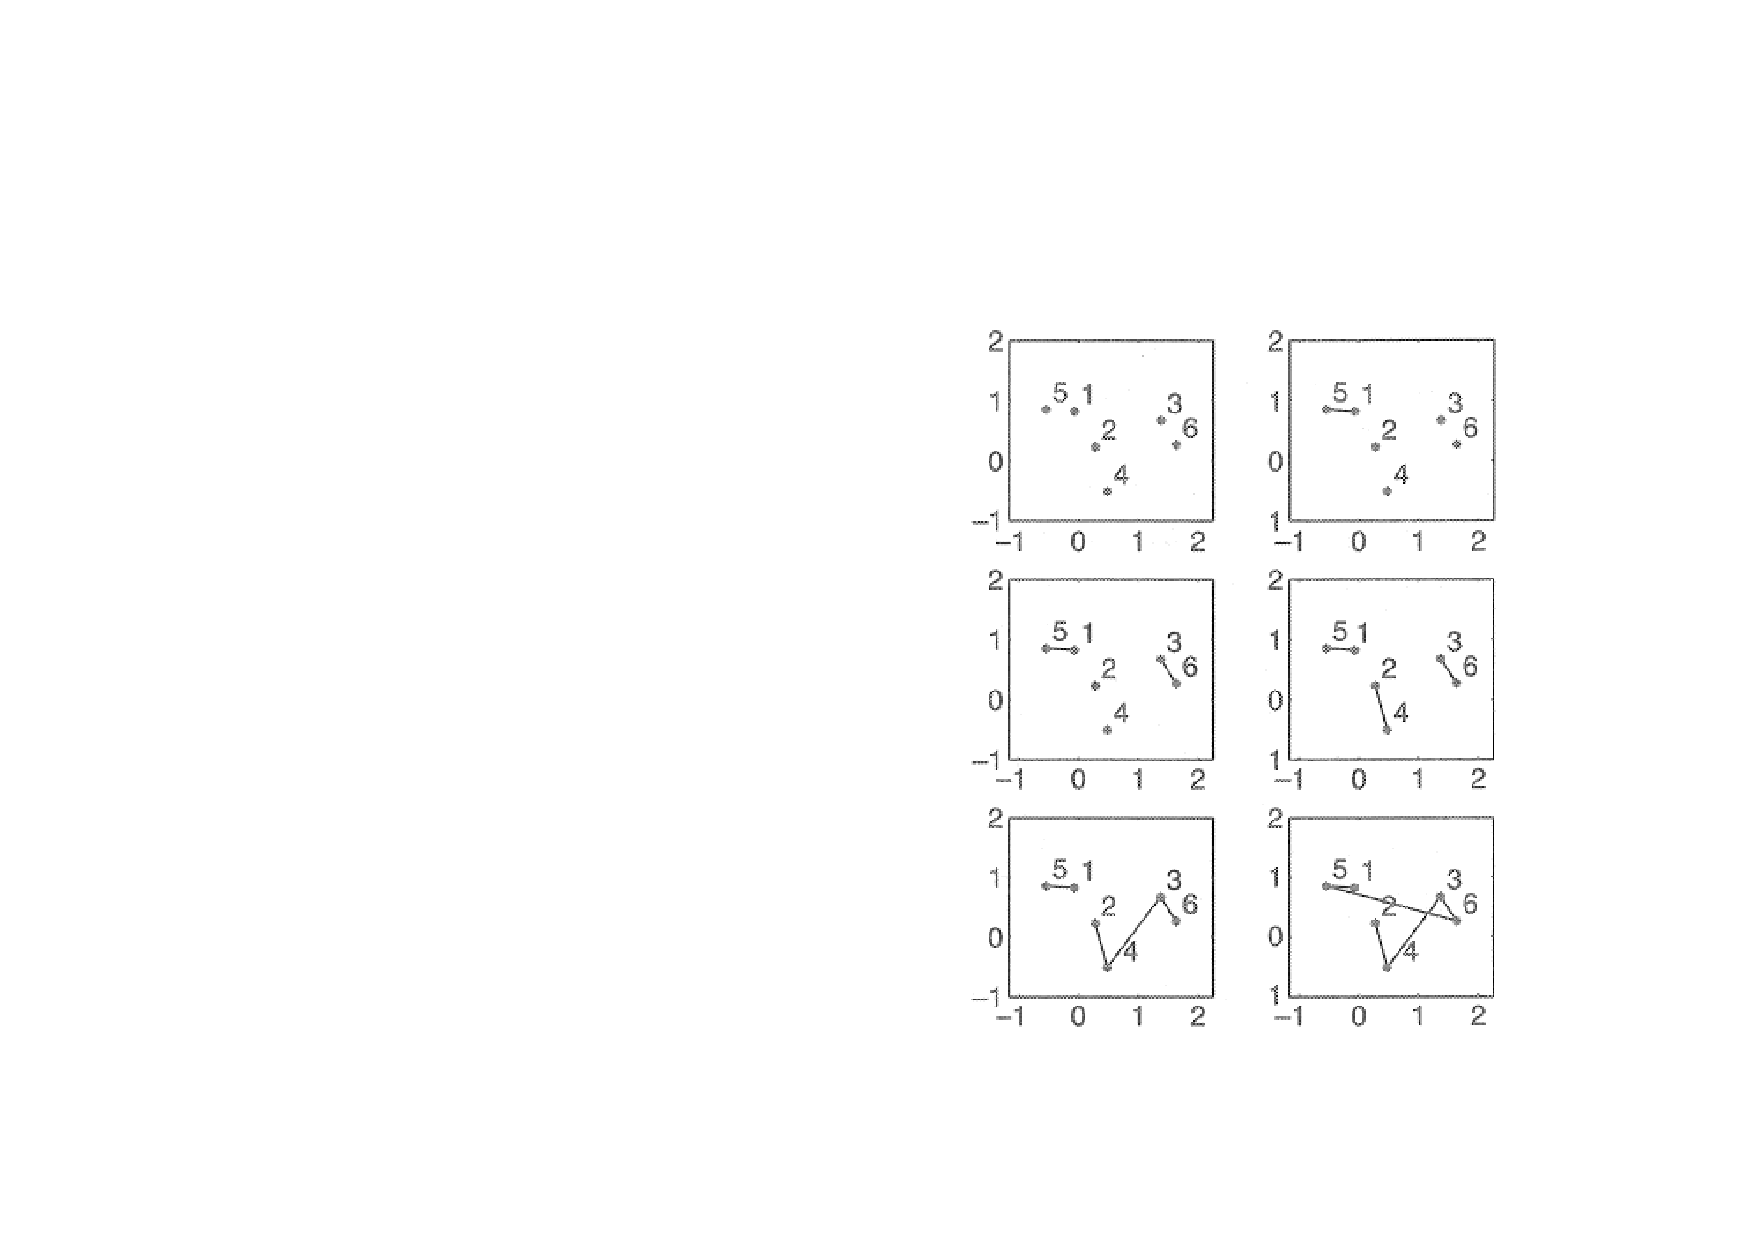
\includegraphics[angle=0,width=0.75\linewidth]{images/unsupervised/hierarchical/hierarchical_complete_link.pdf}
				\caption{Euclidean + Complete-Link}
				%\label{Enel_QQ_Plot_Normal}
			\end{figure}

		\end{columns}

	%\end{block}

\end{frame}


\begin{frame}

	\frametitle{{\color{GradientDescentDiagramGreen}Hierarchical Clustering}}

	%\begin{block}{}

		La gerarchia dei cluster è rappresentata graficamente tramite un dendrogramma.\\
		Il dendogramma mostra a quali distanze i cluster sono raggruppati.

		\begin{columns}

			\column{0.5\linewidth}
			\begin{figure}[!htbp]
				\centering
				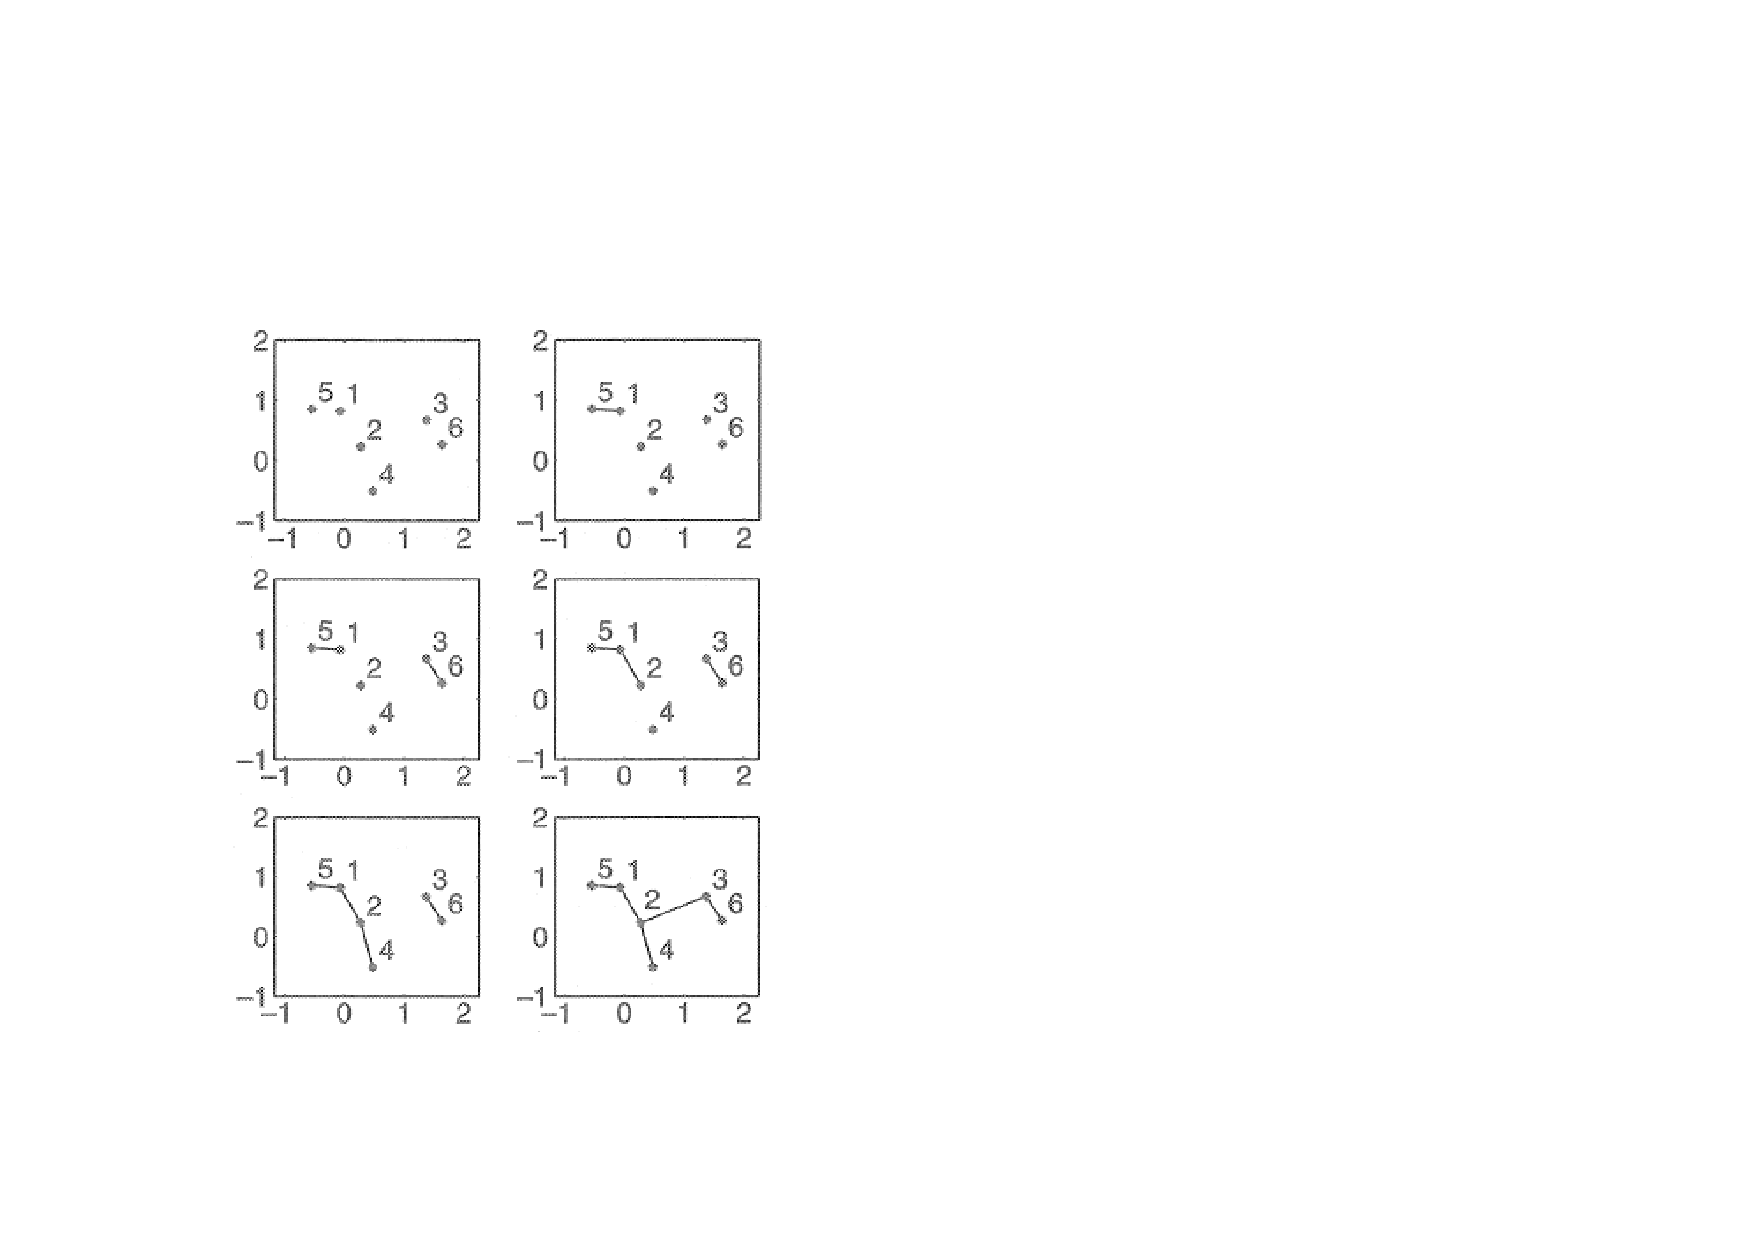
\includegraphics[angle=0,width=0.50\linewidth]{images/unsupervised/hierarchical/hierarchical_single_link.pdf}
				\caption{Single-Link}
				%\label{Enel_HistFit_Normal}
			\end{figure}

			\column{0.5\linewidth}
			\begin{figure}[!htbp]
				\centering
				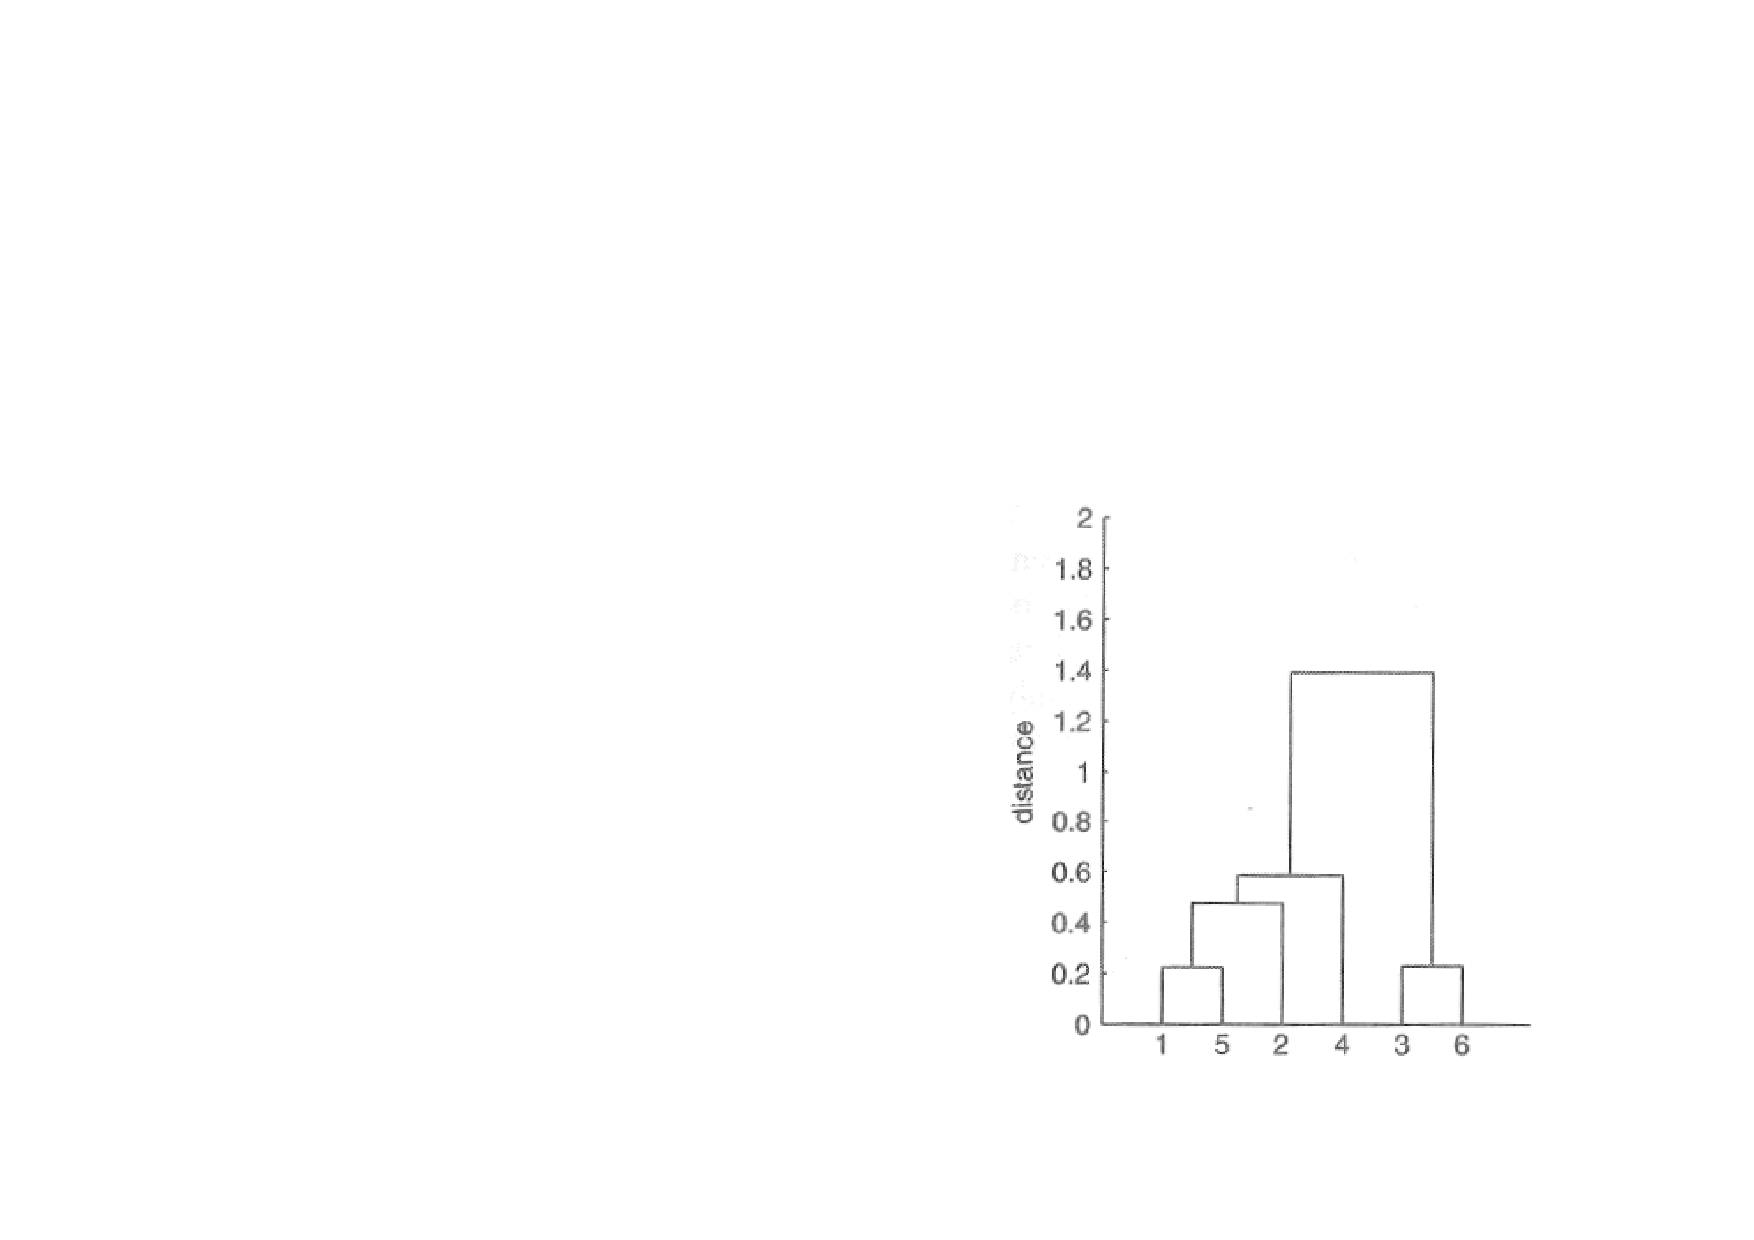
\includegraphics[angle=0,width=0.65\linewidth]{images/unsupervised/hierarchical/hierarchical_single_link_dendogram.pdf}
				\caption{Single-Link Dendogram}
				%\label{Enel_QQ_Plot_Normal}
			\end{figure}

		\end{columns}

	%\end{block}

\end{frame}



\begin{frame}

	\frametitle{{\color{GradientDescentDiagramGreen}Hierarchical Clustering}}

	%\begin{block}{}

		La gerarchia dei cluster è rappresentata graficamente tramite un dendrogramma.\\
		Il dendogramma mostra a quali distanze i cluster sono raggruppati.

		\begin{columns}

			\column{0.5\linewidth}
			\begin{figure}[!htbp]
				\centering
				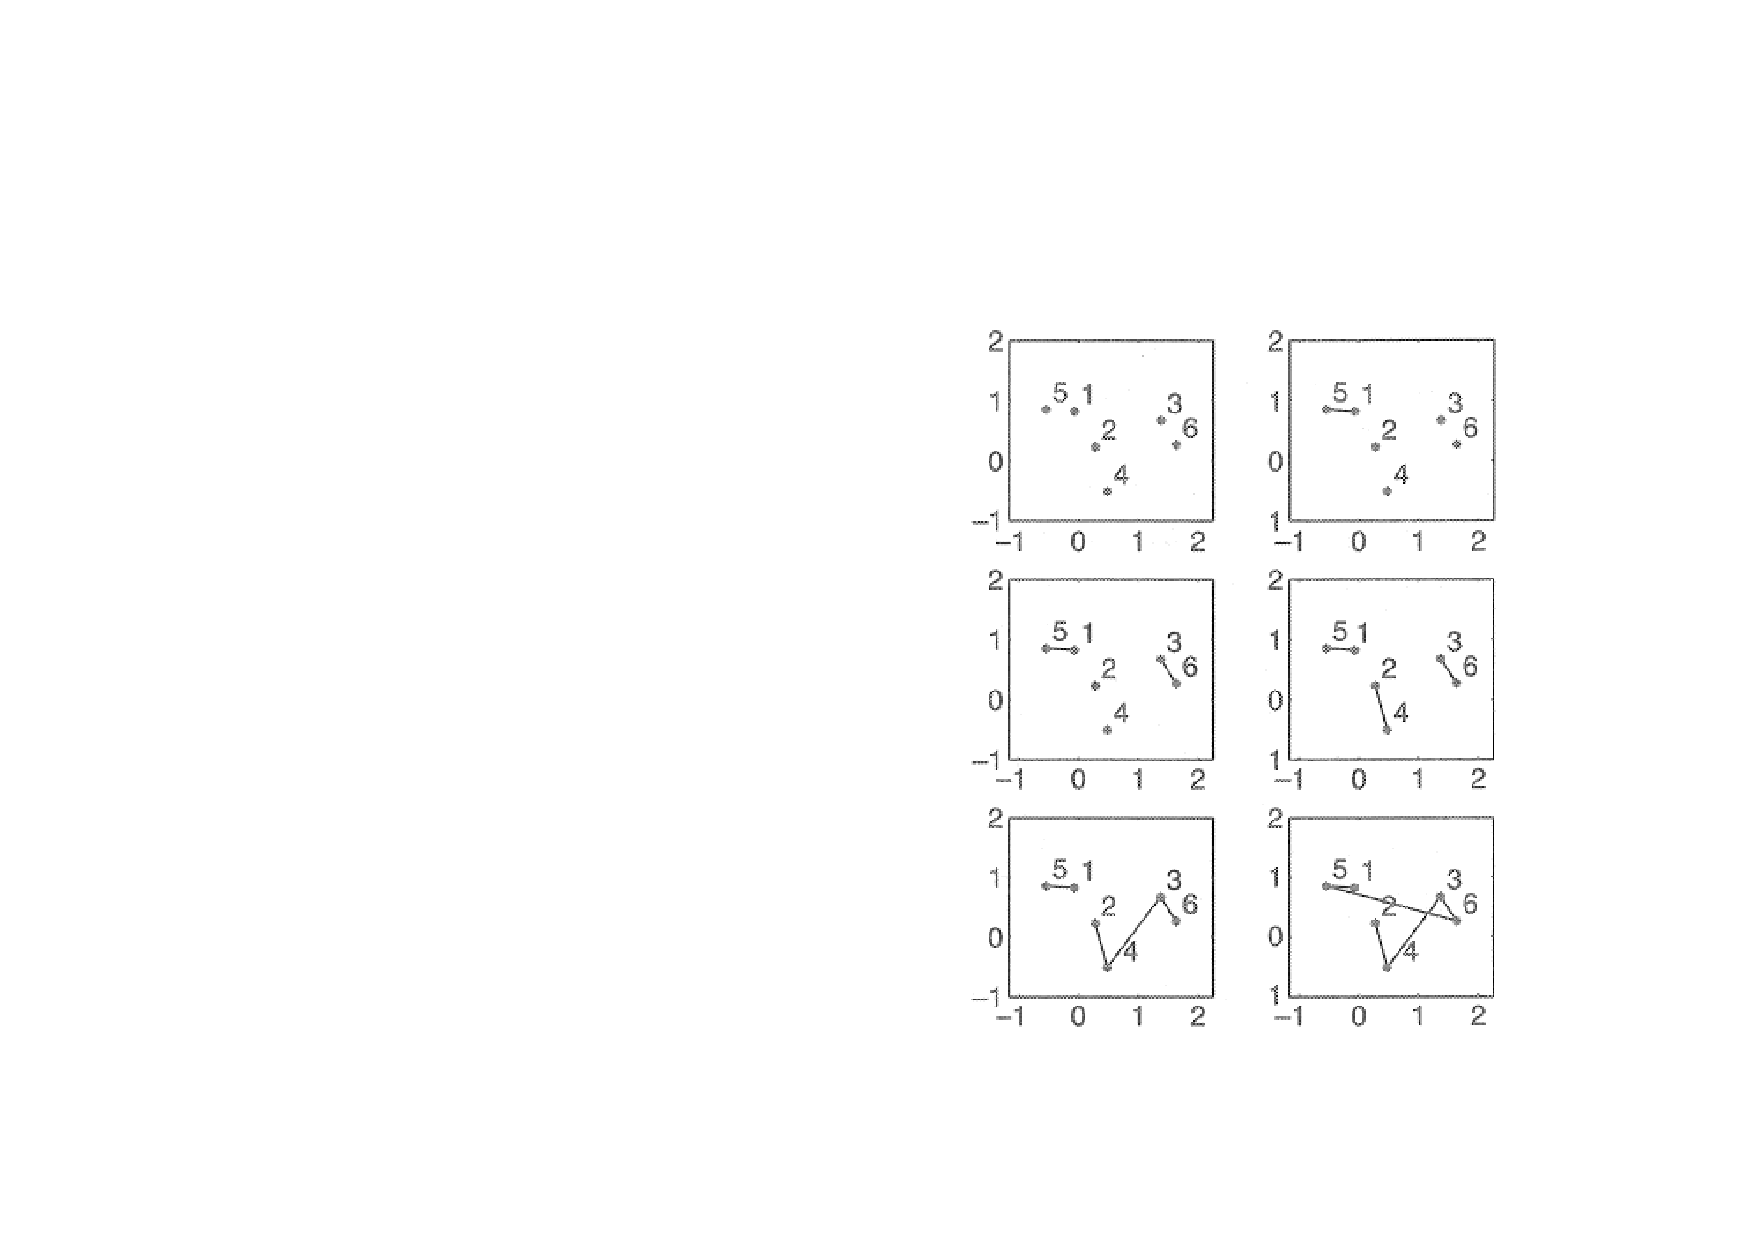
\includegraphics[angle=0,width=0.50\linewidth]{images/unsupervised/hierarchical/hierarchical_complete_link.pdf}
				\caption{Complete-Link}
				%\label{Enel_HistFit_Normal}
			\end{figure}

			\column{0.5\linewidth}
			\begin{figure}[!htbp]
				\centering
				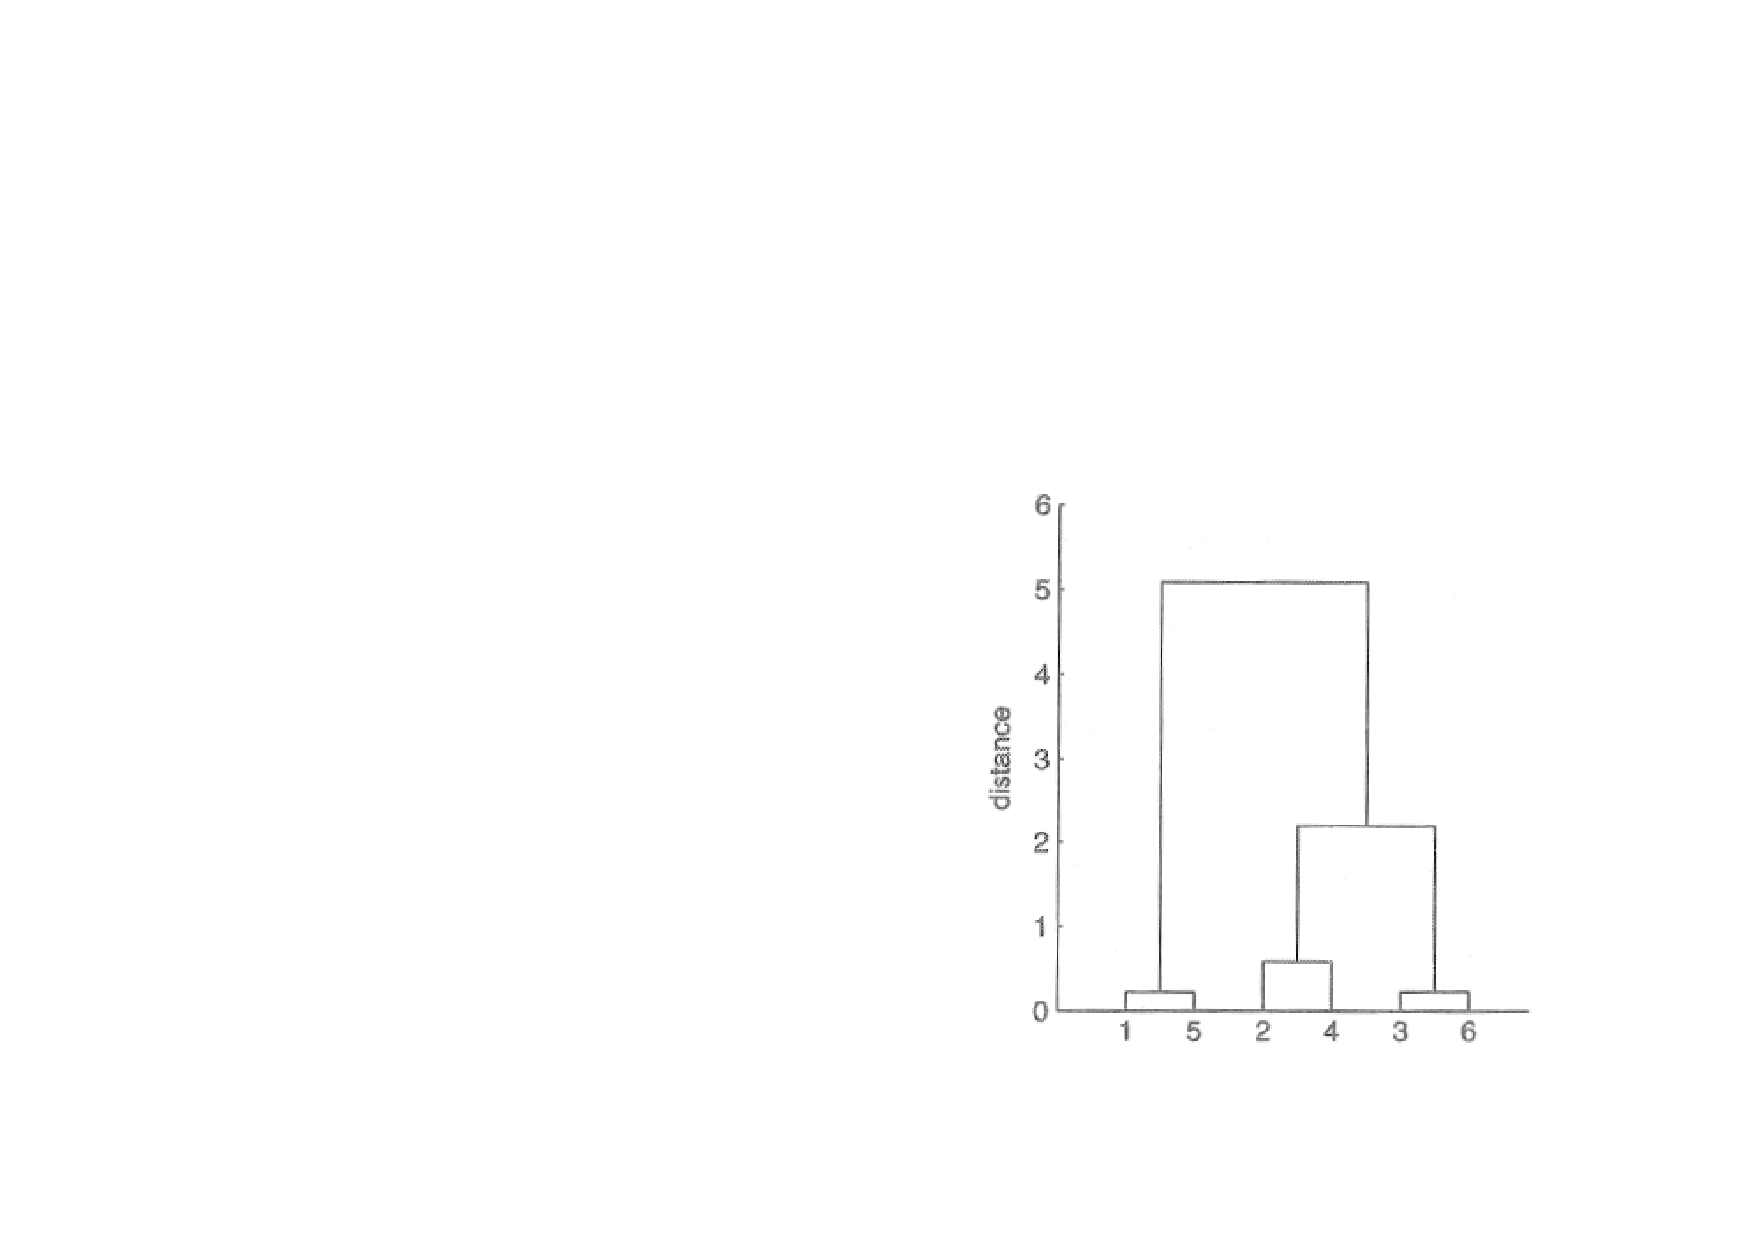
\includegraphics[angle=0,width=0.65\linewidth]{images/unsupervised/hierarchical/hierarchical_complete_link_dendogram.pdf}
				\caption{Complete-Link Dendogram}
				%\label{Enel_QQ_Plot_Normal}
			\end{figure}

		\end{columns}

	%\end{block}

\end{frame}


\begin{frame}

	\frametitle{{\color{GradientDescentDiagramGreen}Hierarchical Clustering}}

	%\begin{block}{}

		I dendrogrammi possono aiutare a identificare un ``buon'' numero di cluster
		\begin{itemize}
			\item un ampio gap nelle distanze suggerisce quando interrompere il processo di raggruppamento
		\end{itemize}

		\begin{columns}

			\column{0.5\linewidth}
			\begin{figure}[!htbp]
				\centering
				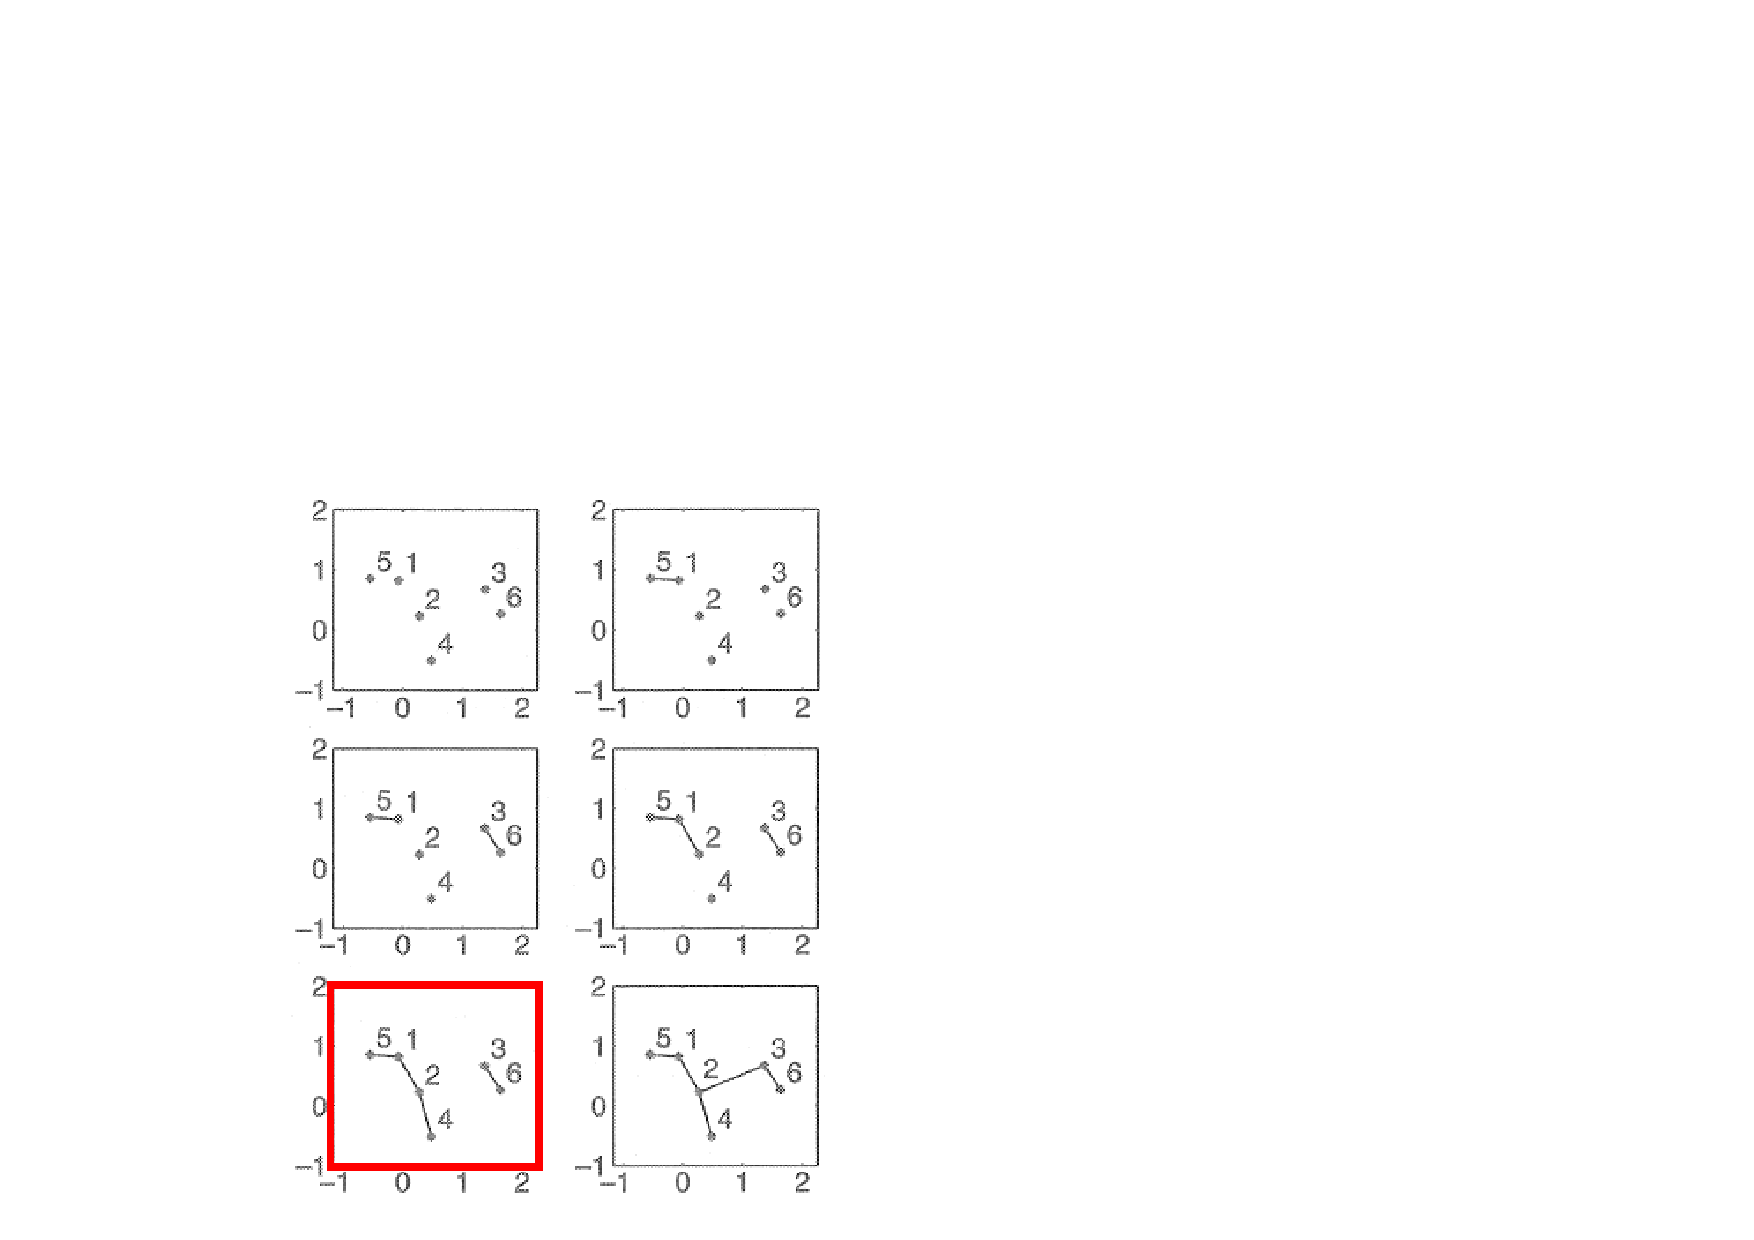
\includegraphics[angle=0,width=0.50\linewidth]{images/unsupervised/hierarchical/hierarchical_single_link_red.pdf}
				\caption{Single-Link Good K}
				%\label{Enel_HistFit_Normal}
			\end{figure}

			\column{0.5\linewidth}
			\begin{figure}[!htbp]
				\centering
				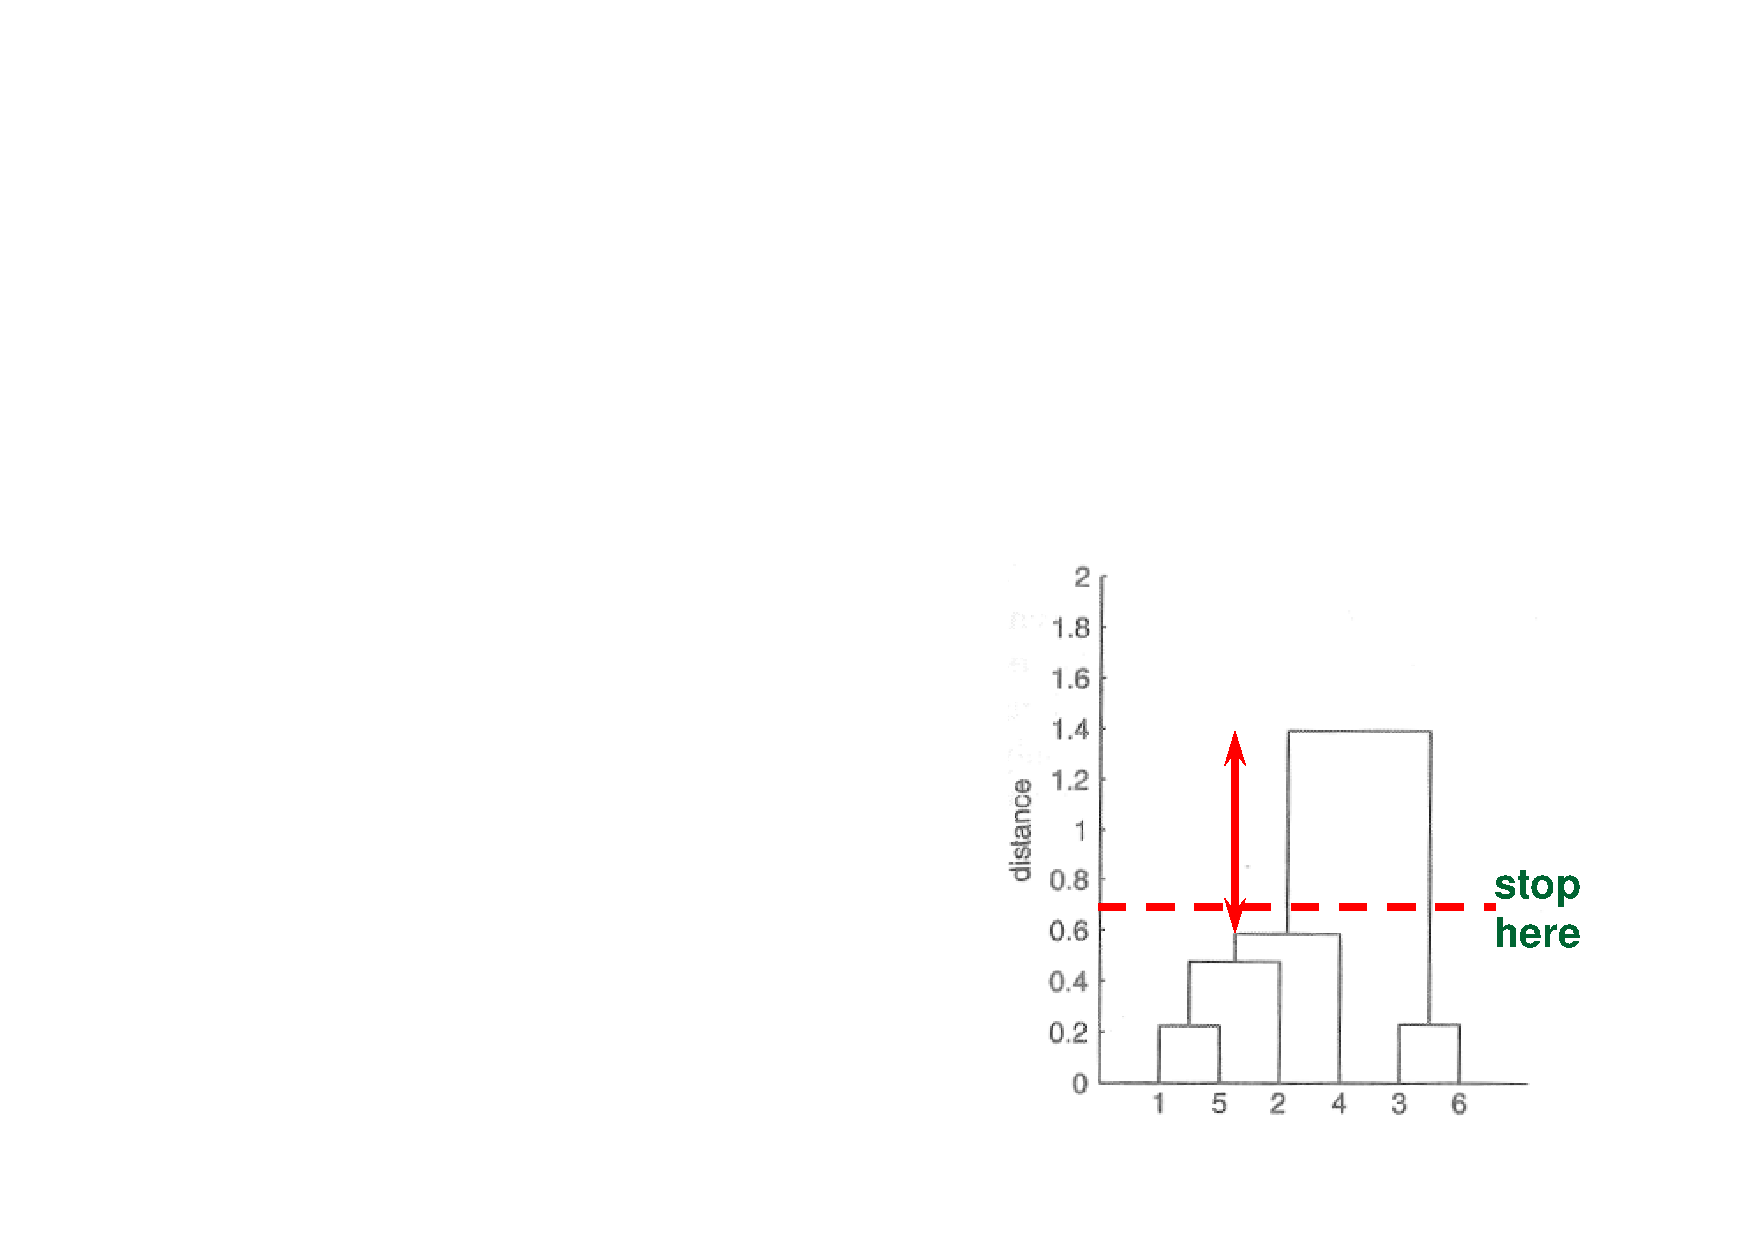
\includegraphics[angle=0,width=0.65\linewidth]{images/unsupervised/hierarchical/hierarchical_single_link_dendogram_red.pdf}
				\caption{Single-Link Dendogram Good K}
				%\label{Enel_QQ_Plot_Normal}
			\end{figure}

		\end{columns}

	%\end{block}

\end{frame}


\begin{frame}

	\frametitle{{\color{GradientDescentDiagramGreen}Hierarchical Clustering}}

	%\begin{block}{}

		Uno svantaggio del \textbf{single-link clustering} è legato al \textbf{chaining}:
		\begin{itemize}
			\item è possibile che si formino cluster allungati che includono punti distanti (aventi poco in comune) attraverso una catena di punti intermedi
			\item in generale, il \textbf{single-link clustering} favorisce la costruzione di cluster isolati, sebbene a volte sia soggetto al chaining
			\item al contrario, l'\textbf{average-} e il \textbf{complete-link} clustering tende a favorire la coesione interna producendo cluster omogenei (spesso sferici)
		\end{itemize}

		\begin{columns}

			\column{0.5\linewidth}
			\begin{figure}[!htbp]
				\centering
				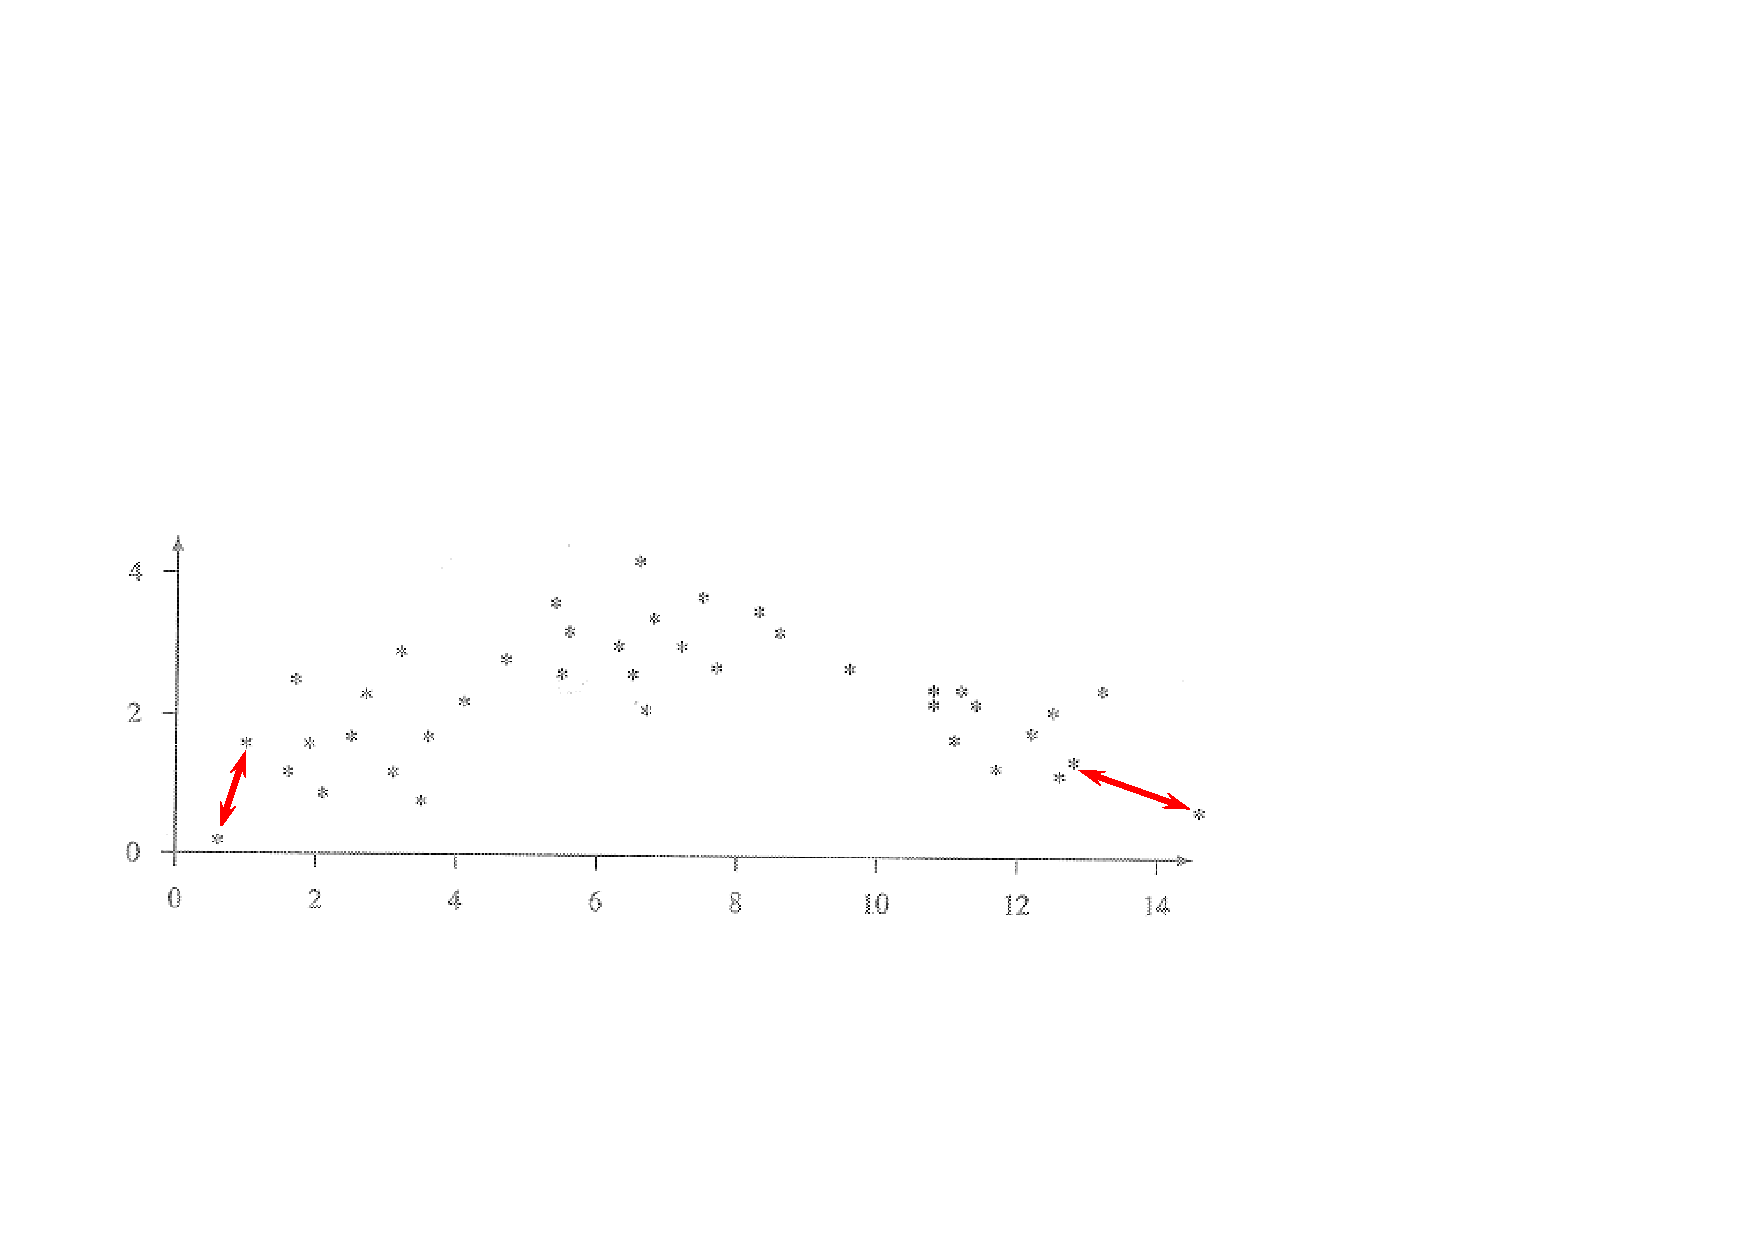
\includegraphics[angle=0,width=1\linewidth]{images/unsupervised/hierarchical/hierarchical_single_link_drawback_1.pdf}
%				\caption{Single-Link Good K}
				%\label{Enel_HistFit_Normal}
			\end{figure}

			\column{0.5\linewidth}
			\begin{figure}[!htbp]
				\centering
				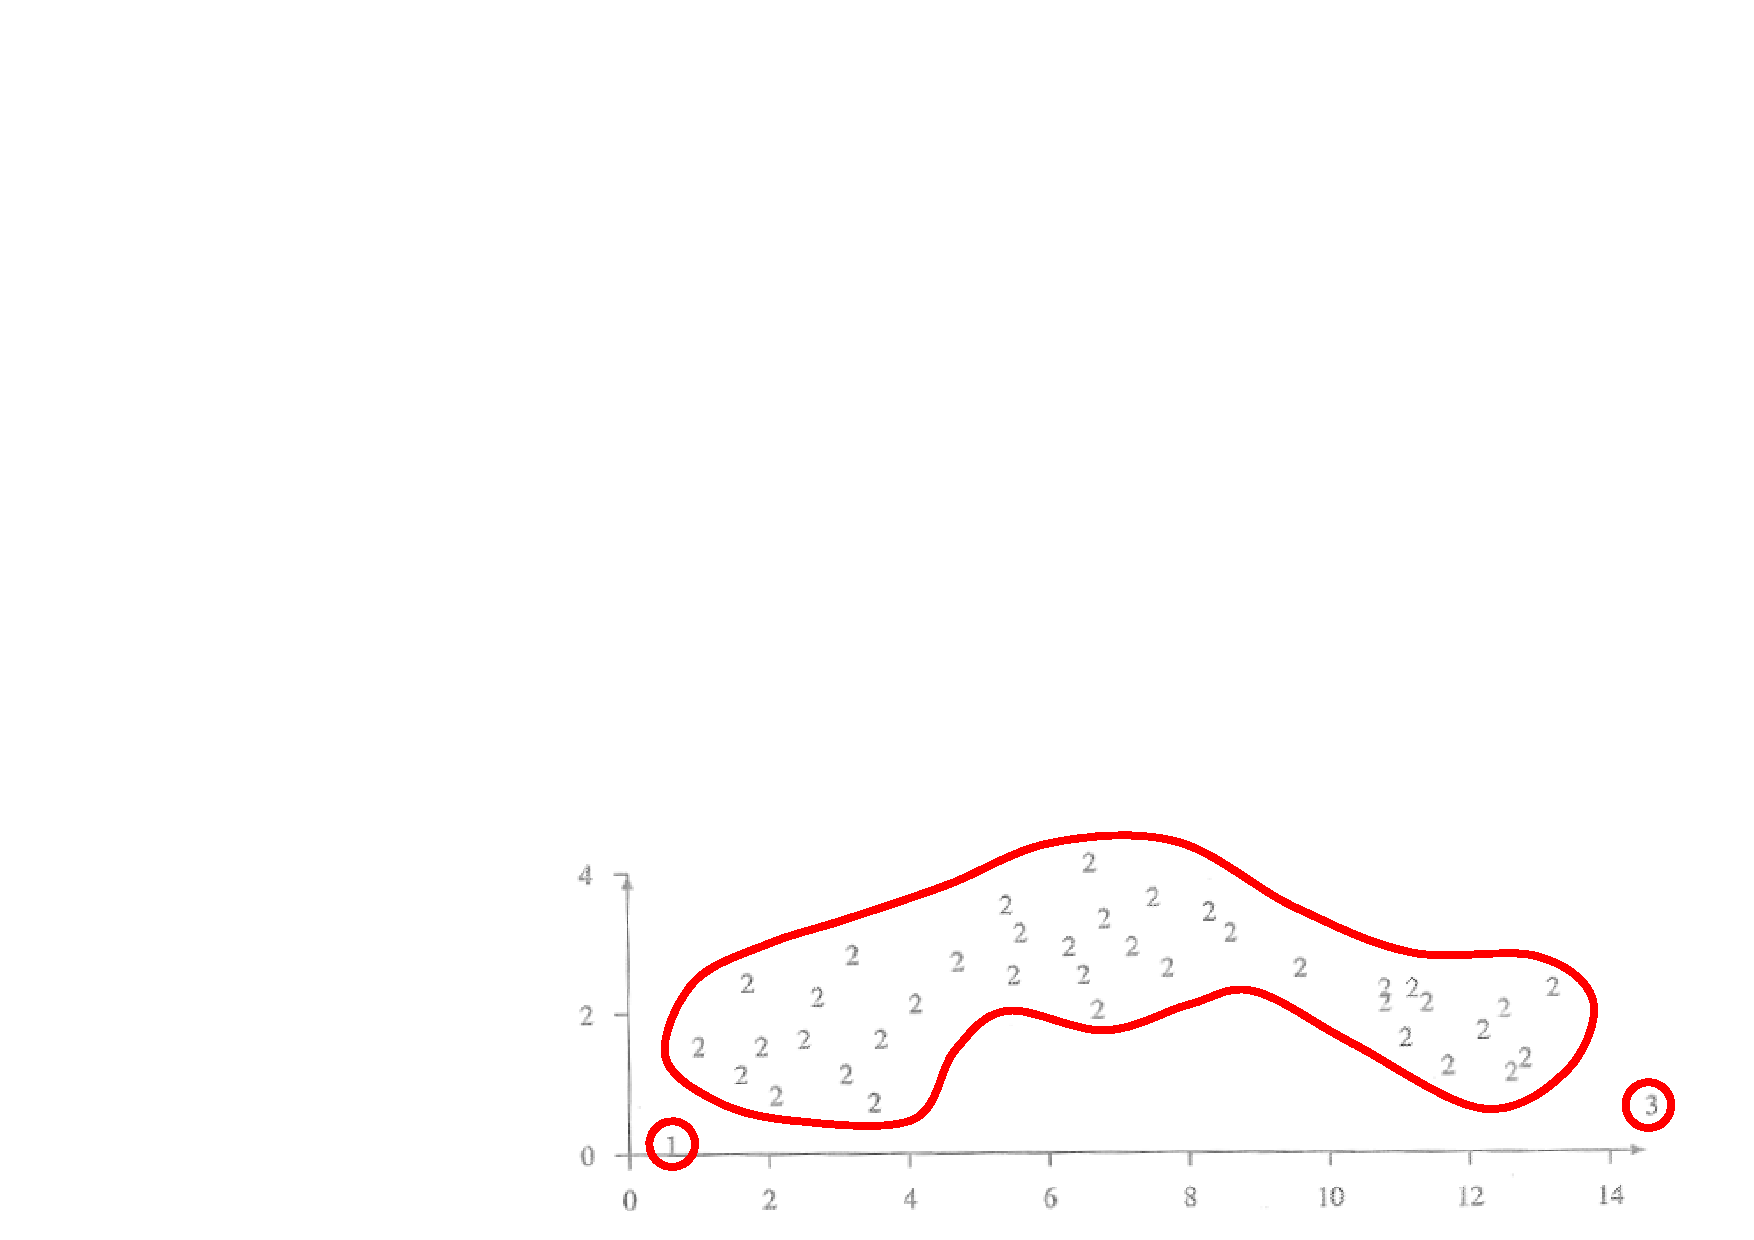
\includegraphics[angle=0,width=1\linewidth]{images/unsupervised/hierarchical/hierarchical_single_link_drawback_2.pdf}
%				\caption{Single-Link Dendogram Good K}
				%\label{Enel_QQ_Plot_Normal}
			\end{figure}

		\end{columns}


	%\end{block}

\end{frame}


\begin{frame}

	\frametitle{{\color{GradientDescentDiagramGreen}Hierarchical Clustering}: segmentazione}
	%\begin{block}{}

		\begin{figure}[!htbp]
			\centering
			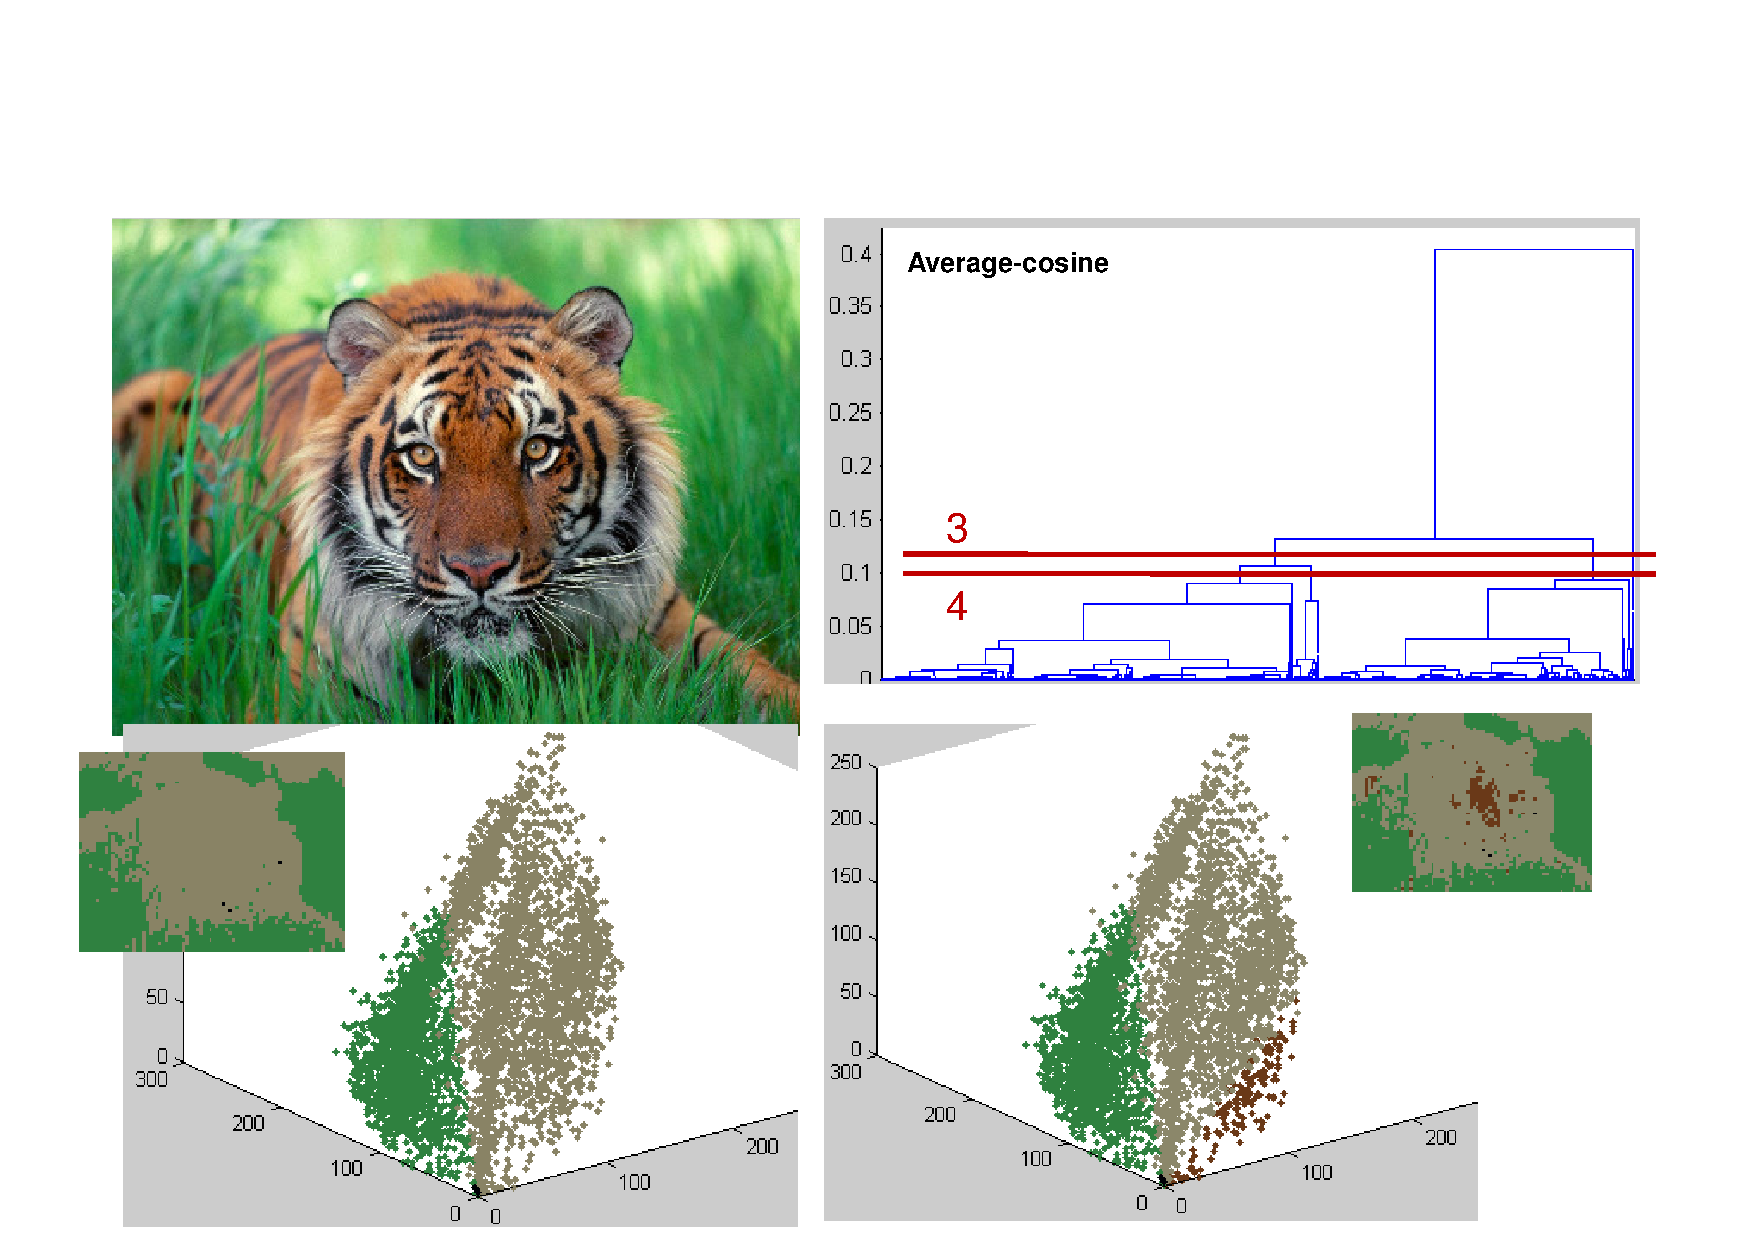
\includegraphics[width=11.0cm]{images/unsupervised/hierarchical/hc_avg_cosine_1.pdf}
			%\caption{Stripe Radar for Fraud Detection}
		\end{figure}

	%\end{block}

\end{frame}

\begin{frame}

	\frametitle{{\color{GradientDescentDiagramGreen}Hierarchical Clustering}: segmentazione}
	%\begin{block}{}

		\begin{figure}[!htbp]
			\centering
			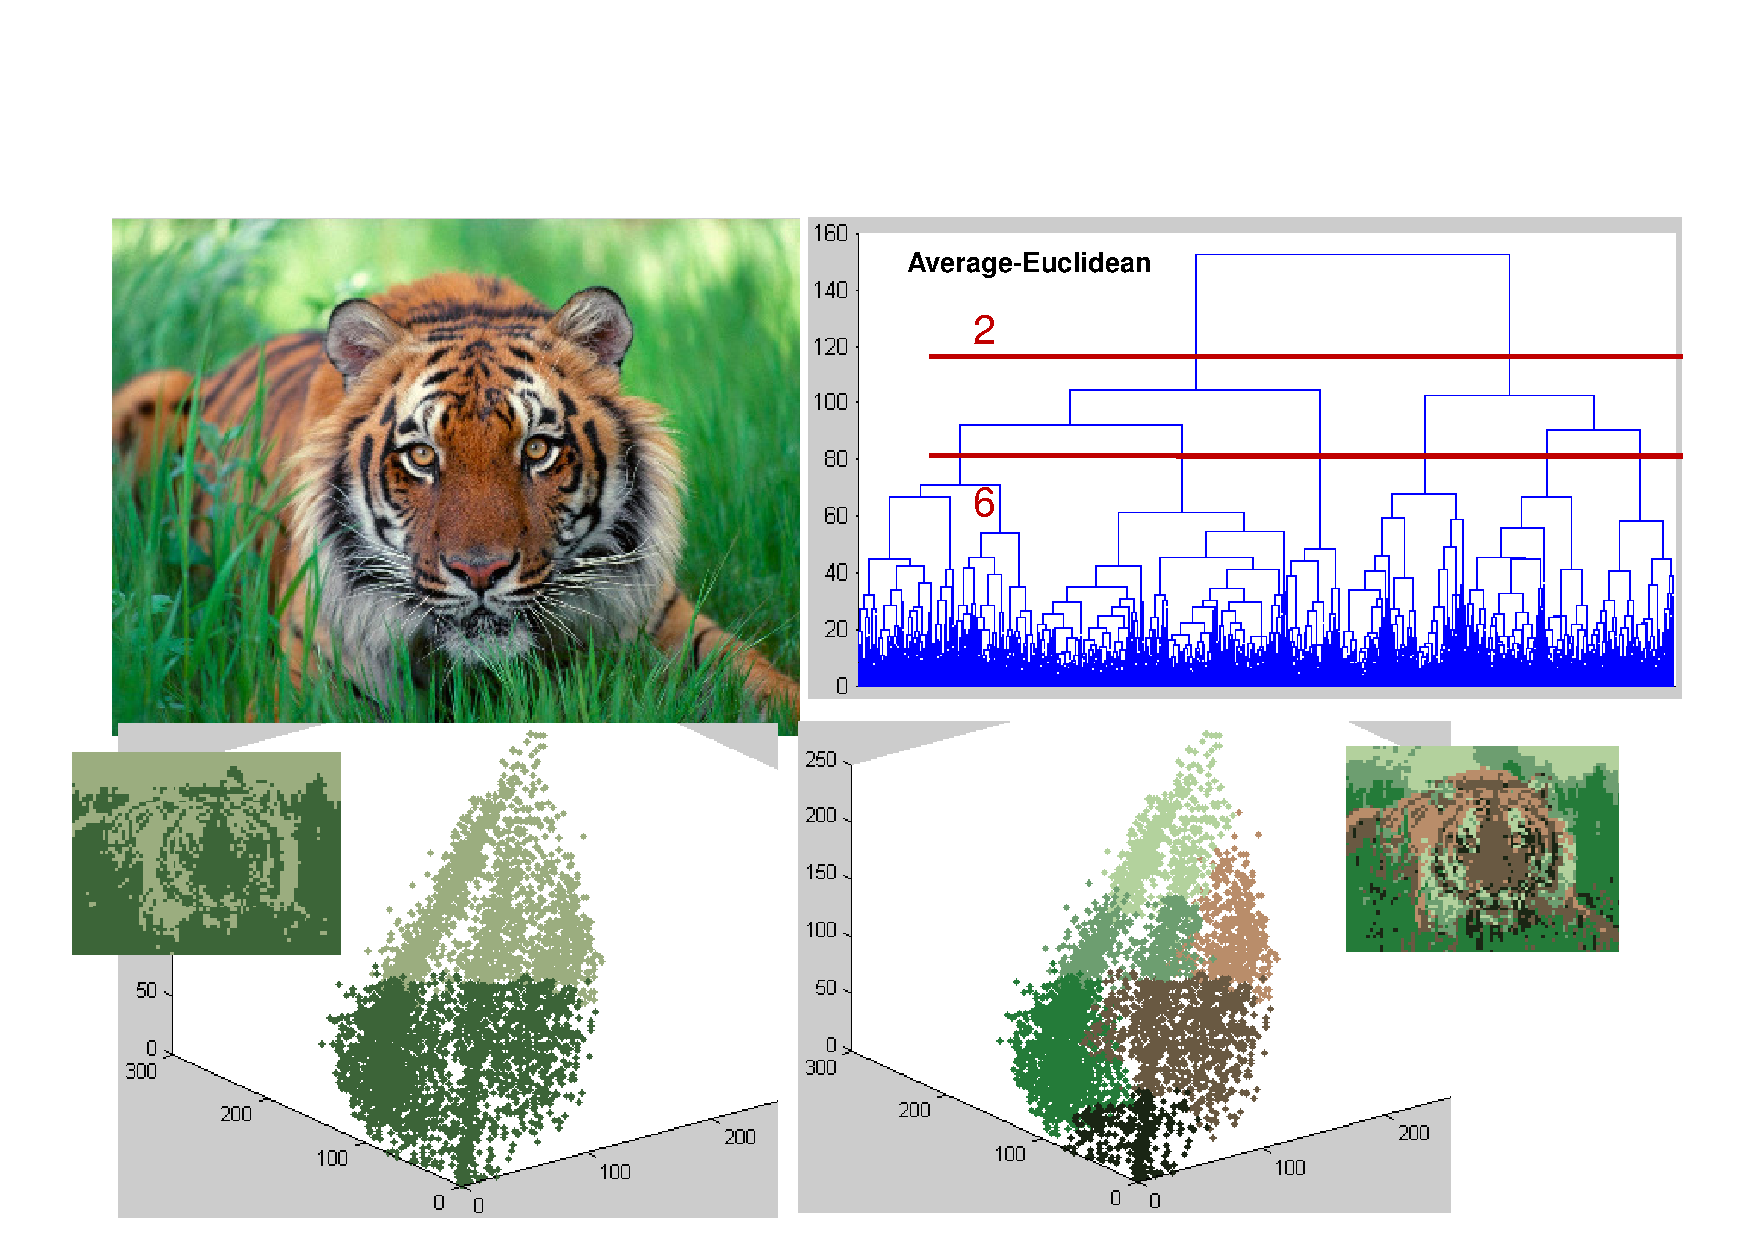
\includegraphics[width=11.0cm]{images/unsupervised/hierarchical/hc_avg_euclidean_1.pdf}
			%\caption{Stripe Radar for Fraud Detection}
		\end{figure}

	%\end{block}

\end{frame}


\begin{frame}

	\frametitle{{\color{GradientDescentDiagramGreen}Hierarchical Clustering}: segmentazione}
	%\begin{block}{}

		\begin{figure}[!htbp]
			\centering
			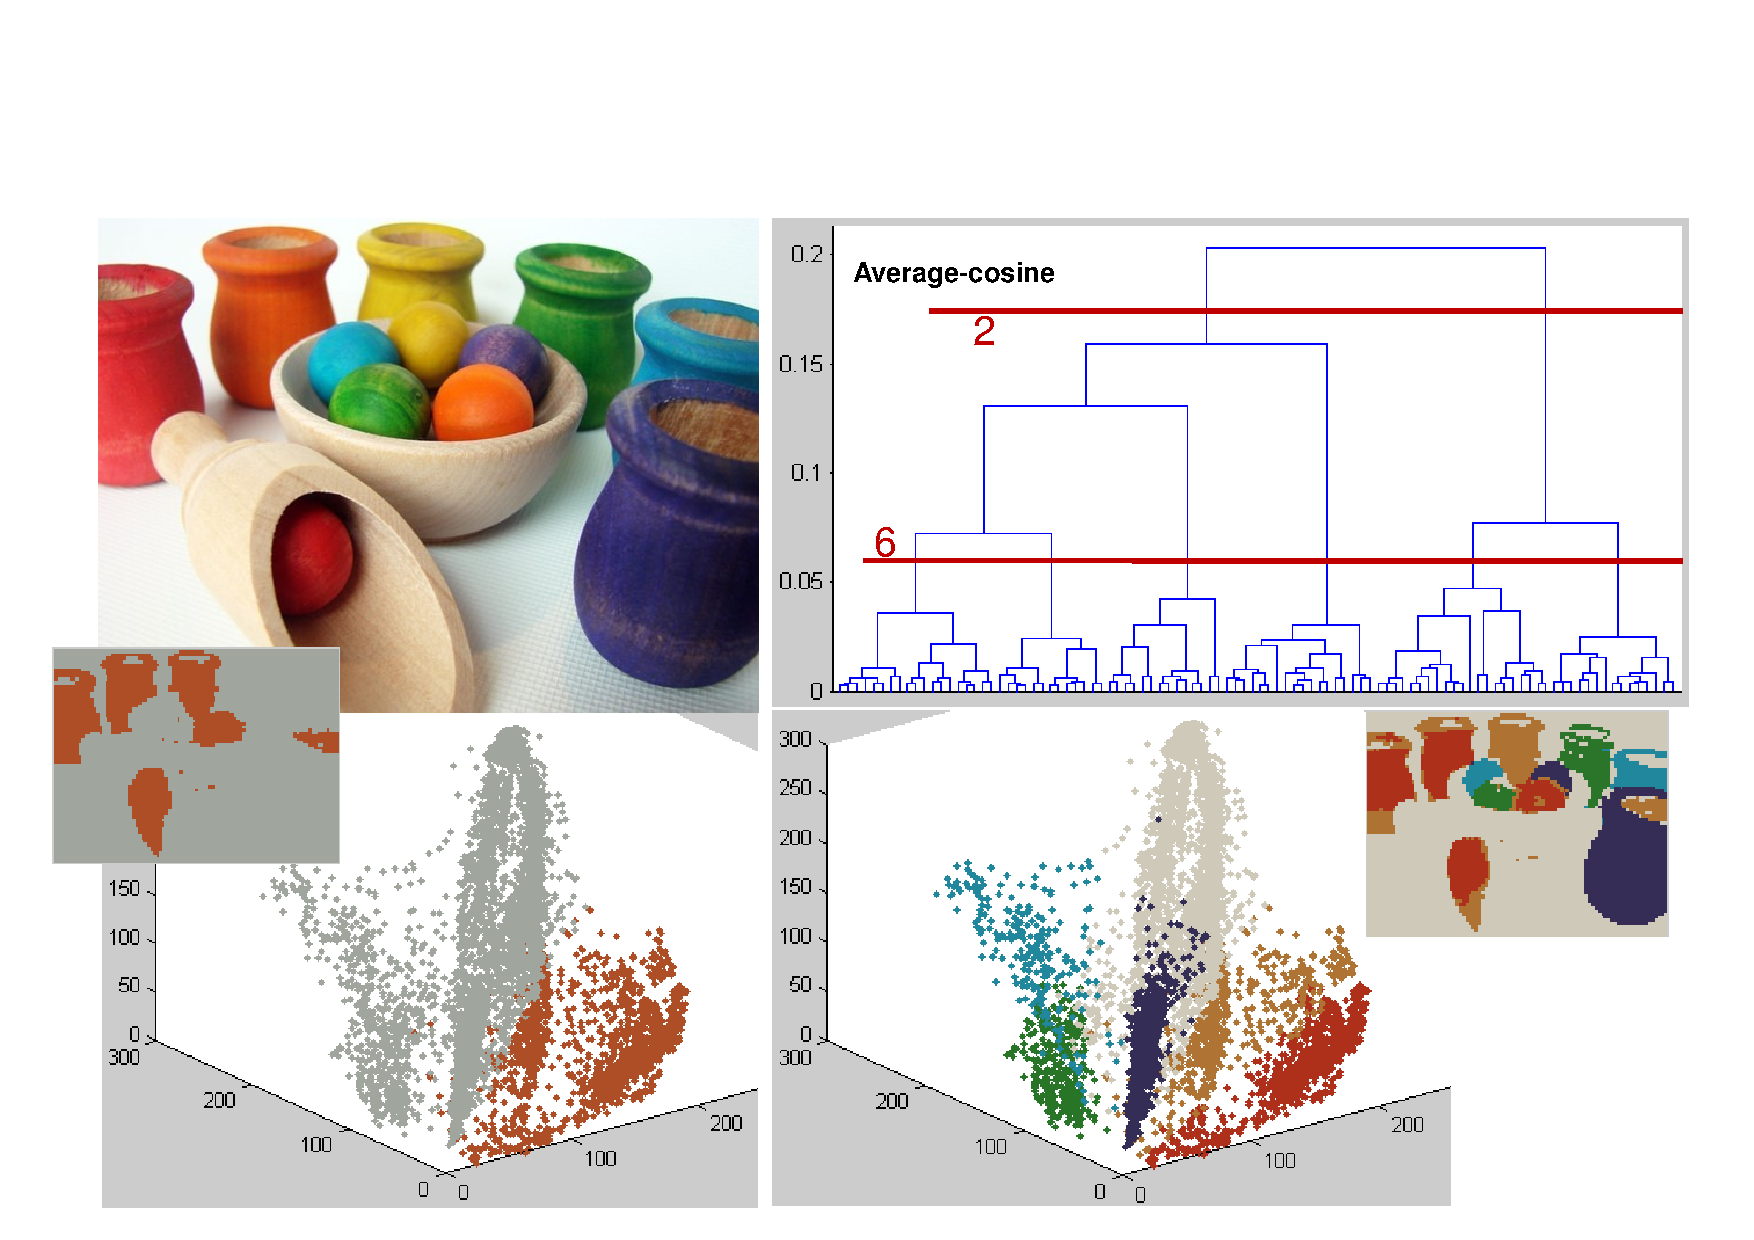
\includegraphics[width=11.0cm]{images/unsupervised/hierarchical/hc_avg_cosine_2.pdf}
			%\caption{Stripe Radar for Fraud Detection}
		\end{figure}

	%\end{block}

\end{frame}


\begin{frame}

	\frametitle{{\color{GradientDescentDiagramGreen}Hierarchical Clustering}: segmentazione}
	%\begin{block}{}

		\begin{figure}[!htbp]
			\centering
			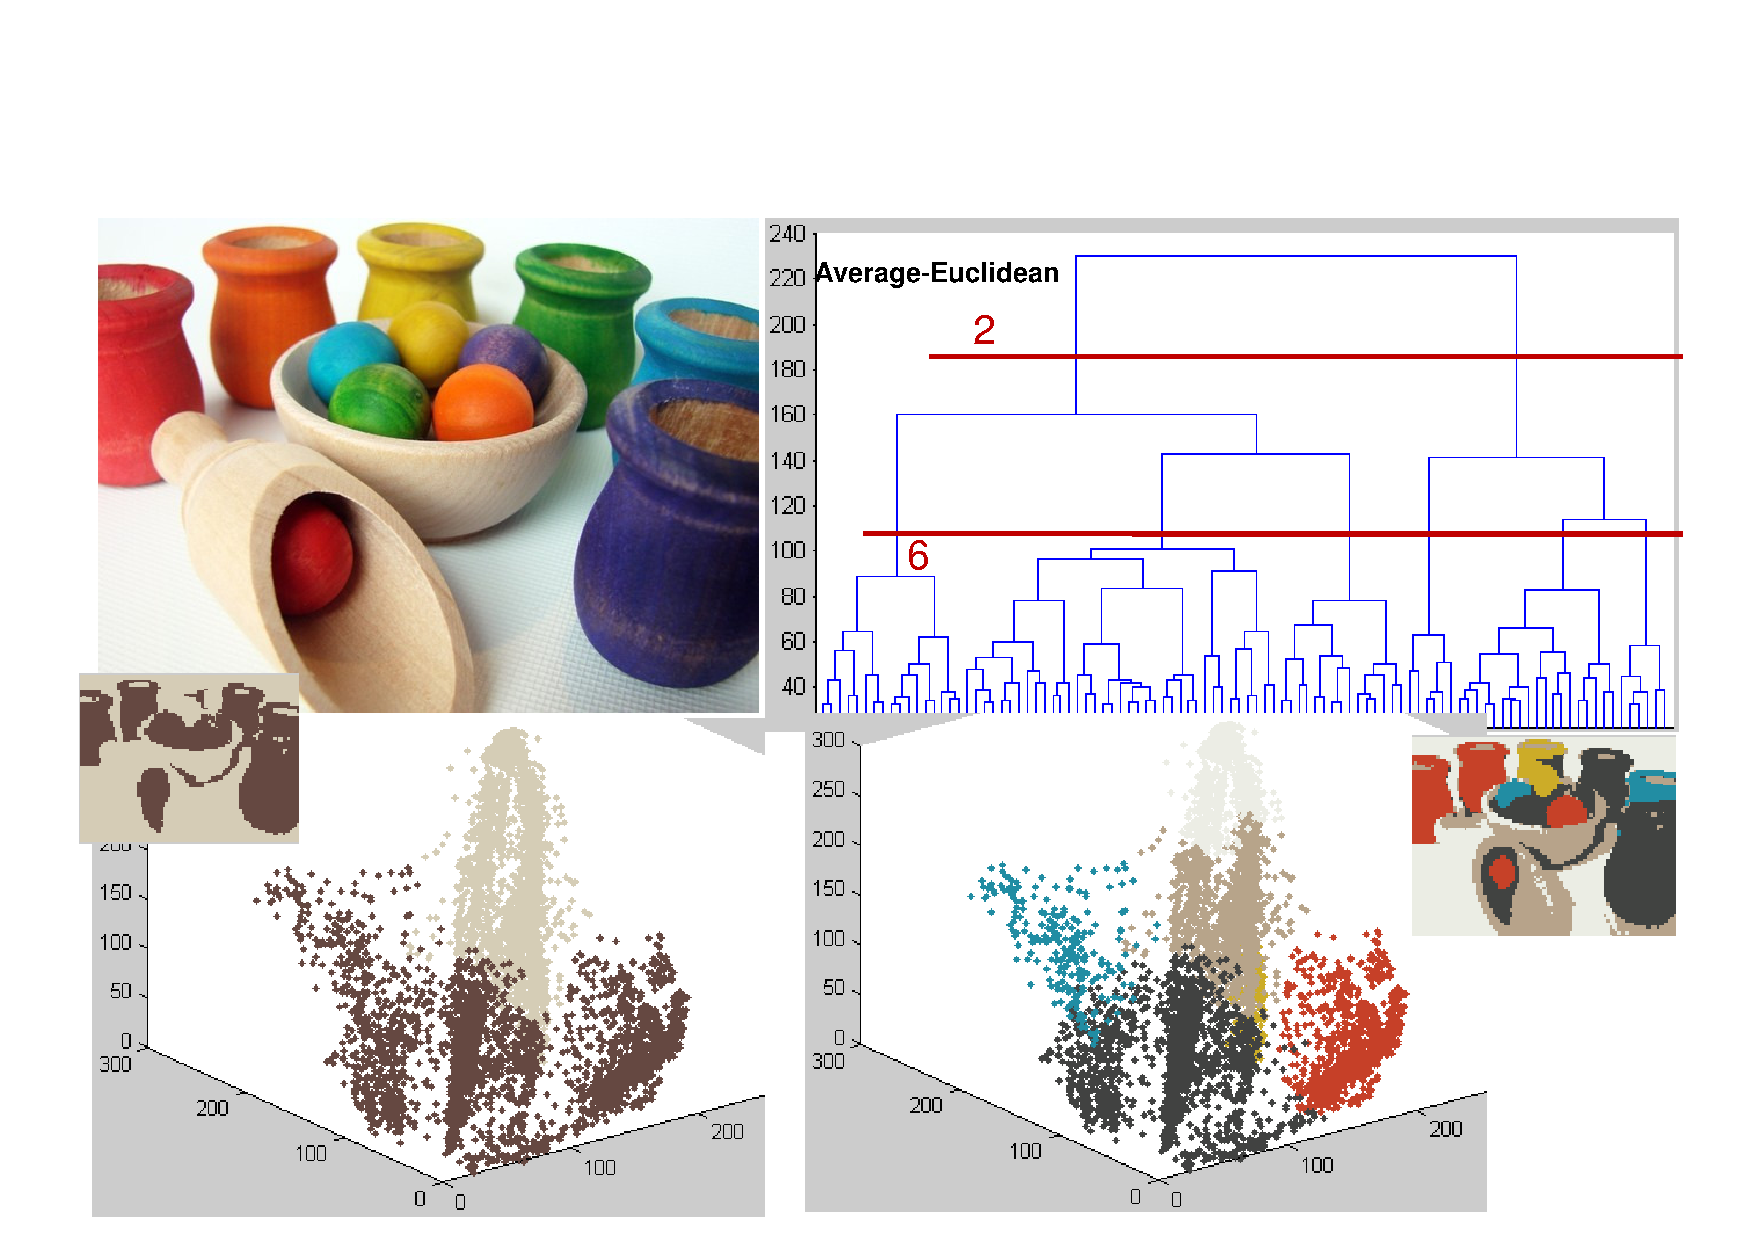
\includegraphics[width=11.0cm]{images/unsupervised/hierarchical/hc_avg_euclidean_2.pdf}
			%\caption{Stripe Radar for Fraud Detection}
		\end{figure}

	%\end{block}

\end{frame}


\begin{frame}

	\frametitle{{\color{GradientDescentDiagramGreen}Hierarchical Clustering}: pro e contro}
	%\begin{block}{}

		Pro e contro del clustering gerarchico:
		\begin{itemize}
			\item la procedura di clustering non richiede la definizione del numero di cluster
			\item la procedura di clustering produce relazioni gerarchiche tra i cluster
			\item non viene fornita un'identificazione esplicita del numero ottimale di clusters
			\item a seconda della strategia di linkage (in particolare single-link), sono possibili cluster eterogenei (chaining). In questi casi, rappresentare dei cluster con un unico punto è fuorviante
			\item gli algoritmi di clustering gerarchico agglomerativo o divisivo esaminano tutte le coppie di punti\ifthenelse{\boolean{highschool}}{}{ e hanno complessità rispettivamente di $O(n^2log(n))$ e $O(n^2)$}.
		\end{itemize}
	%\end{block}

\end{frame}


\subsubsection[Distribution-based (GMM)]{Distribution-based \textit{(GMM)}}
\begin{frame}

	\frametitle{{\color{GradientDescentDiagramOrange}Distribution-based Clustering}, in sintesi}

	%\begin{block}{}
		Il distribution-based clustering presuppone che i dati siano composti da distribuzioni, come le distribuzioni gaussiane.
		\newlinedouble
		Nella figura, il distribution-based clustering clusterizza i dati in tre distribuzioni gaussiane.
		All'aumentare della distanza dal centro della distribuzione, la probabilità che un punto appartenga alla distribuzione diminuisce.\\
		Le bande mostrano che la probabilità diminuisce. Se non conosci il tipo di distribuzione nei tuoi dati, dovresti usare un algoritmo diverso.
		\begin{figure}[!htbp]
			\centering
			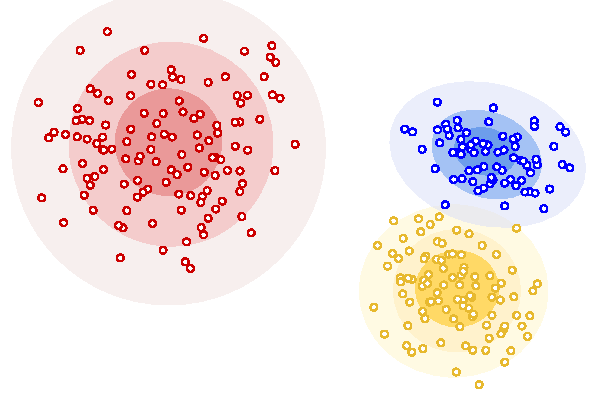
\includegraphics[width=5.0cm]{images/unsupervised/types/Clustering_Distribution.pdf}
					%\caption{Stripe Radar for Fraud Detection}
		\end{figure}
	%\end{block}

\end{frame}


\begin{frame}

	\frametitle{{\color{GradientDescentDiagramOrange}Distribution-based Clustering}: Mixture of Gaussian}

		\begin{columns}

			\column{0.55\linewidth}
			\begin{itemize}
				\item con il clustering K-means, la forma dei cluster è sempre la stessa: sferica attorno al centro del cluster
				\item una soluzione più flessibile è consentire alla forma di ciascun cluster di conformarsi a una gaussiana multivariata
				\item la distribuzione dei dati è modellata da una mistura di distribuzioni gaussiane (\textbf{mixture of Gaussian}), ogni cluster corrispondente a un componente della mistura
					\begin{itemize}
						\item[--] ogni cluster è caratterizzato non solo da una media $\mu_k$, ma anche da una matrice di covarianza $C_k$
					\end{itemize}
			\end{itemize}

			\column{0.45\linewidth}
			\begin{figure}[!htbp]
				\centering
				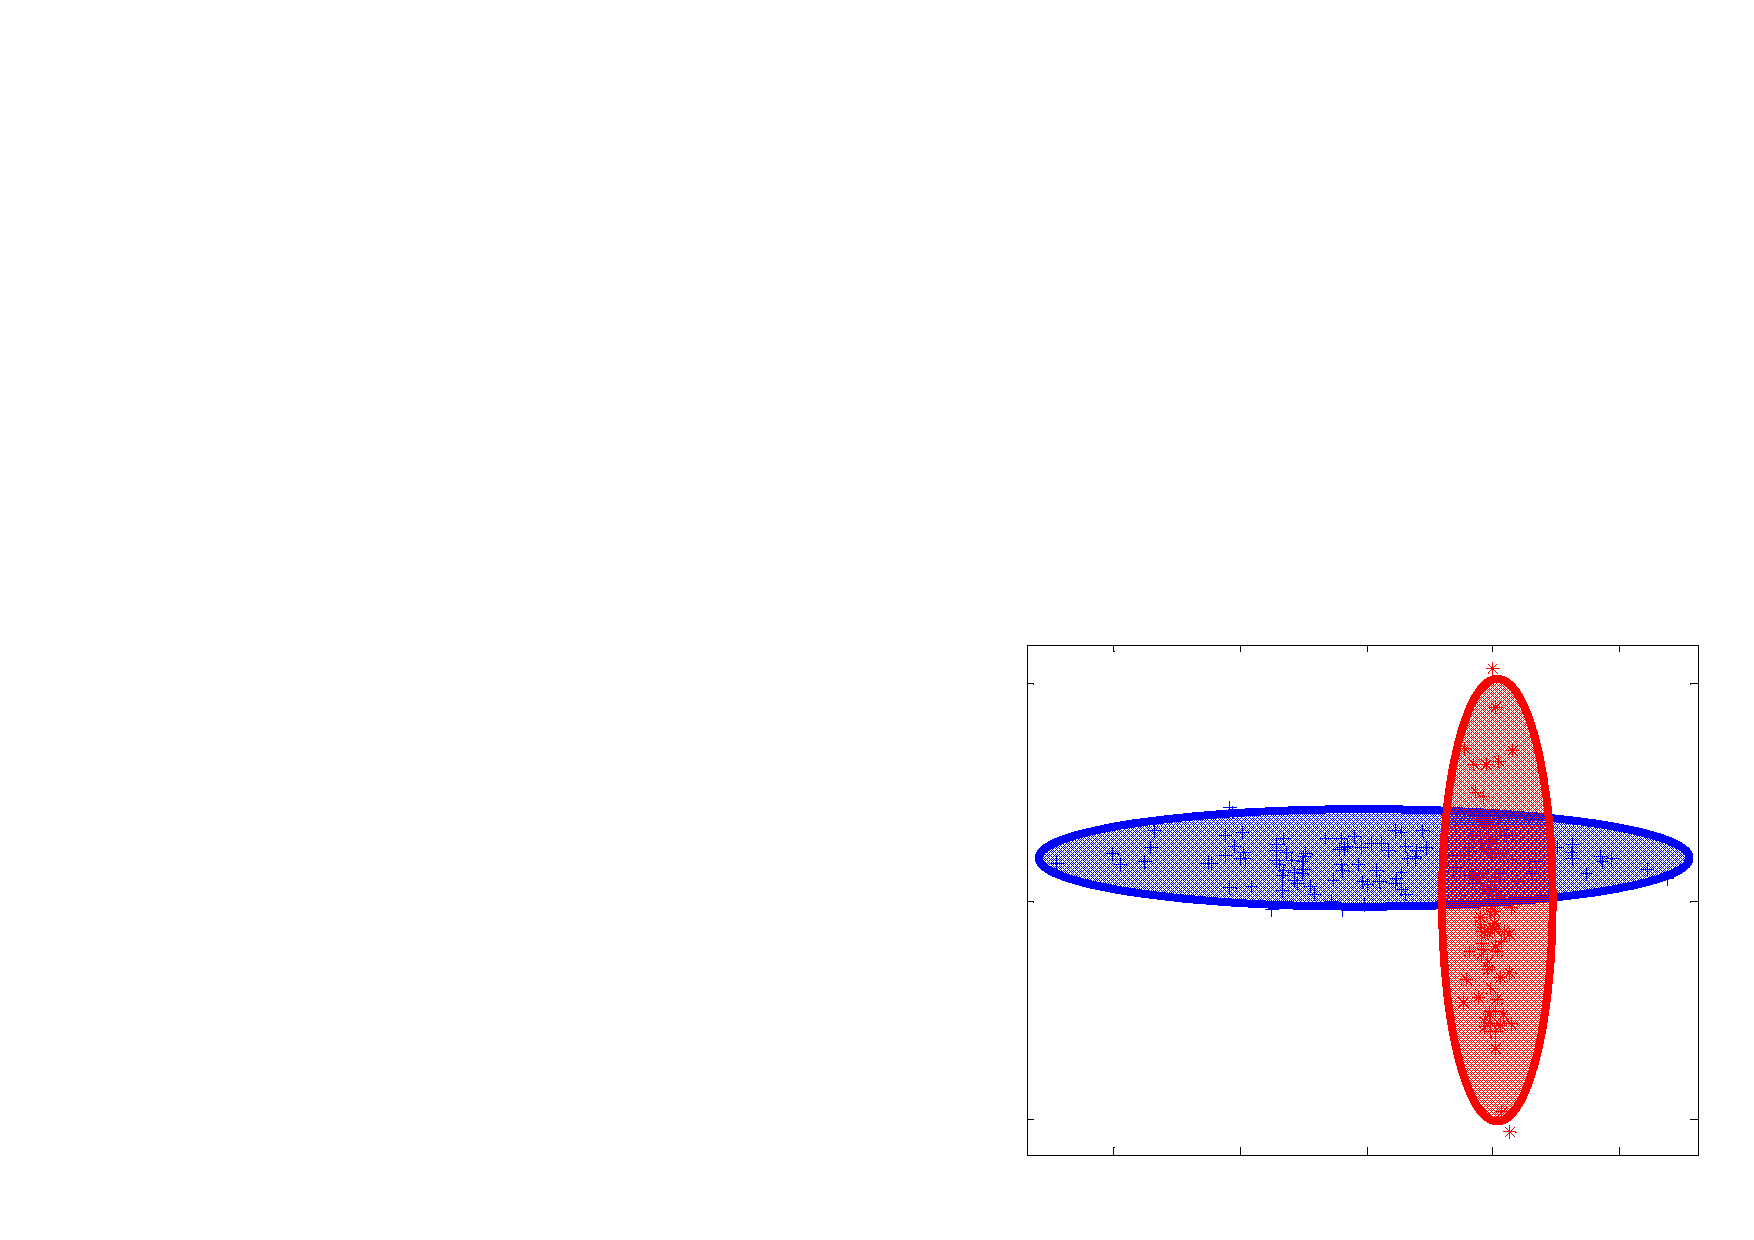
\includegraphics[angle=0,width=1.0\linewidth]{images/unsupervised/gaussian_mixture/gmm_example.pdf}
	%				\caption{Single-Link Dendogram Good K}
				%\label{Enel_QQ_Plot_Normal}
			\end{figure}

		\end{columns}
	%\end{block}

\end{frame}


\ifthenelse{\boolean{highschool}}{

\begin{frame}

	\frametitle{{\color{GradientDescentDiagramOrange}Distribution-based Clustering}: Mixture of Gaussian 1D}

	\begin{block}{Distribuzione gaussiana (o normale o Gauss o Laplace-Gauss)}
%		\begin{itemize}			
			\begin{columns}

				\column{0.37\linewidth}
				$$\mathcal{N}(x\vert\mu, \sigma)= {\frac{1}{\sigma\sqrt{2\pi}}}e^{- {\frac {1}{2}} (\frac {x-\mu}{\sigma})^2}$$
				\begin{scriptsize}
					\begin{itemize}
						\item $\mathcal{N}(\cdot)	=$ densità di probabilità
						\item $\mu =$ media
						\item $\sigma^2 =$ varianza
						\item $\sigma =$	 deviazione standard
					\end{itemize}
					$\qquad$ \underline{\href{https://academo.org/demos/gaussian-distribution/}{Prova con differenti $\mu$ e $\sigma$}}
				\end{scriptsize}

					
				\column{0.63\linewidth}
				\begin{figure}[!htbp]
					\centering
					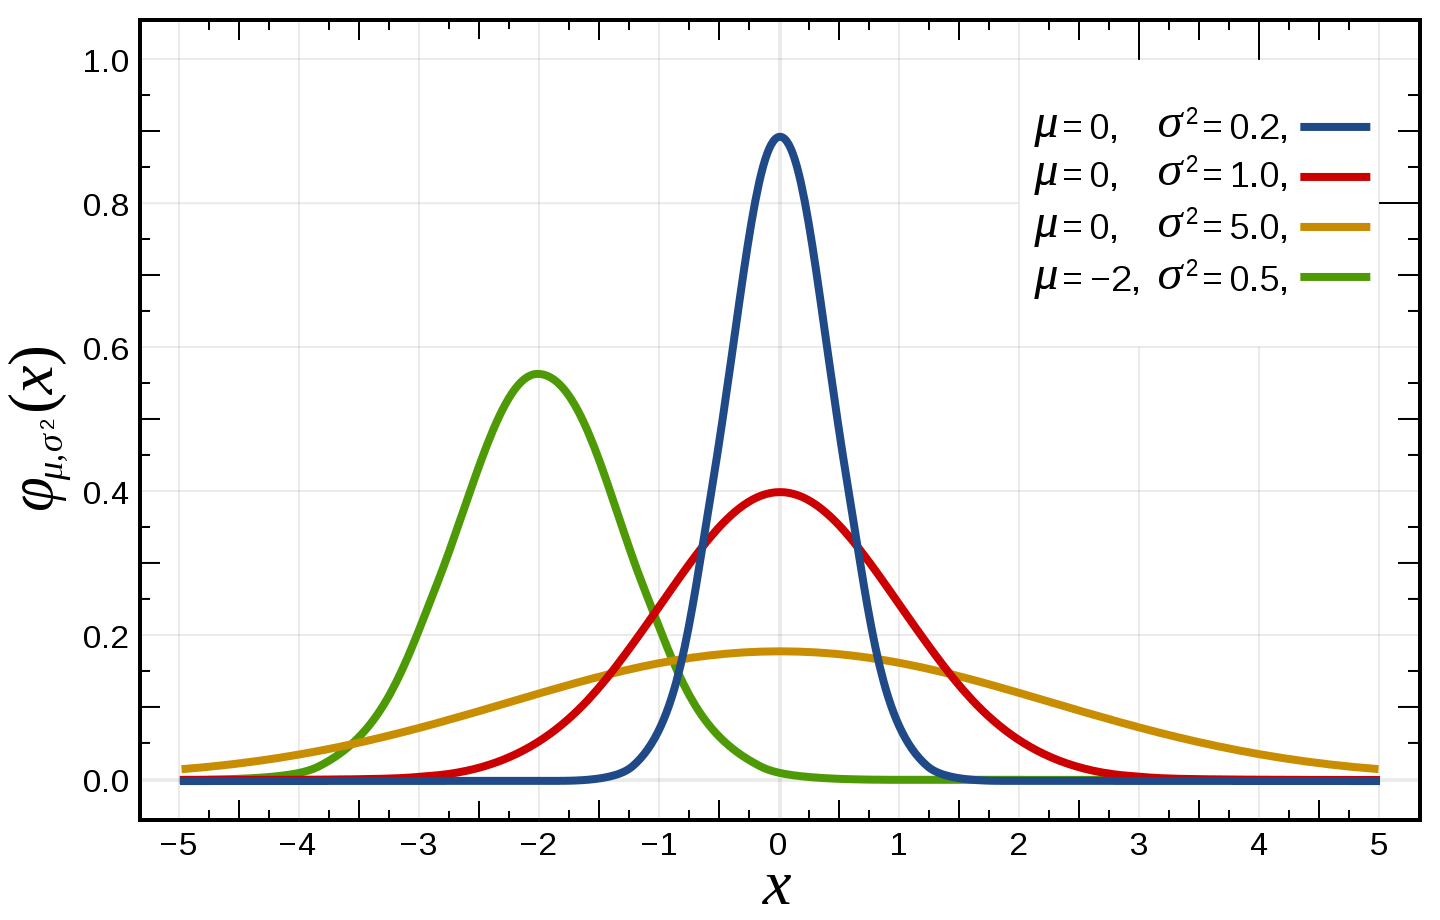
\includegraphics[angle=0,width=1.0\linewidth]{images/unsupervised/gaussian_mixture/gaussian_pdf.png}
		%				\caption{Single-Link Dendogram Good K}
					%\label{Enel_QQ_Plot_Normal}
				\end{figure}
			\end{columns}

%		\end{itemize}
	\end{block}

\end{frame}


\begin{frame}

	\frametitle{{\color{GradientDescentDiagramOrange}Distribution-based Clustering}: Mixture of Gaussian 1D}	

	\begin{block}{Es \#1: un assaggio dell'idea; clusterizzare un dataset con singola feature:}

		\begin{figure}[!htbp]
			\centering
			
			% Foto salvate da una simulazione fatta qui:
			% http://sia.webpopix.org/mixtureModels.html
			\includegraphics<1>[width=0.70\linewidth, height=6.2cm]{images/unsupervised/gaussian_mixture/gmm_idea_0.png}
			\includegraphics<2>[width=0.70\linewidth, height=6.2cm]{images/unsupervised/gaussian_mixture/gmm_idea_1.png}
			\includegraphics<3>[width=0.70\linewidth, height=6.2cm]{images/unsupervised/gaussian_mixture/gmm_idea_2.png}
			\includegraphics<4>[width=0.70\linewidth, height=6.2cm]{images/unsupervised/gaussian_mixture/gmm_idea_3.png}
			%\caption{Single-Link}
			%\label{Enel_HistFit_Normal}
		\end{figure}

	\end{block}

\end{frame}


\begin{frame}

	\frametitle{{\color{GradientDescentDiagramOrange}Distribution-based Clustering}: Mixture of Gaussian 1D}	
	\begin{block}{Es \#2: un assaggio dell'idea; clusterizzare un dataset con singola feature:}
		\centering
		\animategraphics[controls={play, step, stop}, height=5.5cm]{2.0}{images/unsupervised/gaussian_mixture/gmm_1D_K_2/gmm_1D_K_2-}{0}{32}
	\end{block}
		
\end{frame}


\begin{frame}

	\frametitle{{\color{GradientDescentDiagramOrange}Distribution-based Clustering}: Mixture of Gaussian 1D}	
	\begin{block}{Es \#3: un assaggio dell'idea; clusterizzare un dataset con singola feature:}
		\centering
		\animategraphics[controls={play, step, stop}, height=5.5cm]{2.0}{images/unsupervised/gaussian_mixture/gmm_1D_K_3/gmm_1D_K_3-}{0}{41}
	\end{block}
		
\end{frame}


\begin{frame}

	\frametitle{{\color{GradientDescentDiagramOrange}Distribution-based Clustering}: Mixture of Gaussian MultiD}

	\begin{block}{Il passaggio da 1$D$ a 2$D$:}
%		\begin{itemize}
			
			\begin{columns}
				\column{0.45\linewidth}
				\begin{figure}[!htbp]
					\centering
					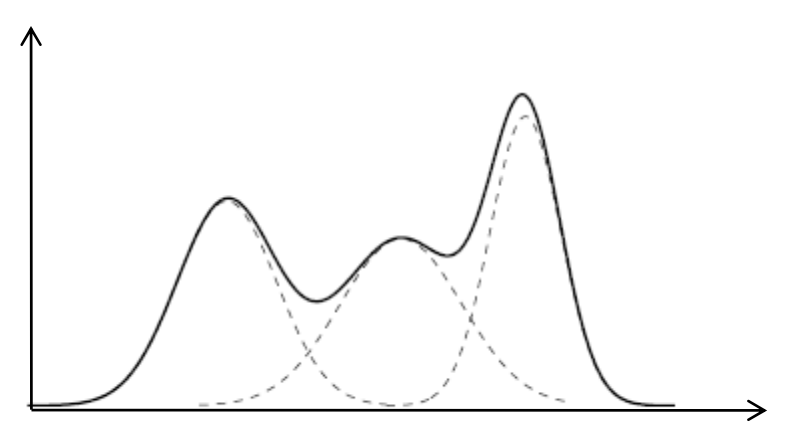
\includegraphics[width=0.85\linewidth]{images/unsupervised/gaussian_mixture/gmm_monovariate.png}
					\caption{GMM applicato su D=1}
				\end{figure}
					
				\column{0.1\linewidth}
				$\rightarrow$
				
				\pause
				
				\column{0.45\linewidth}
				\begin{figure}[!htbp]
					\centering
					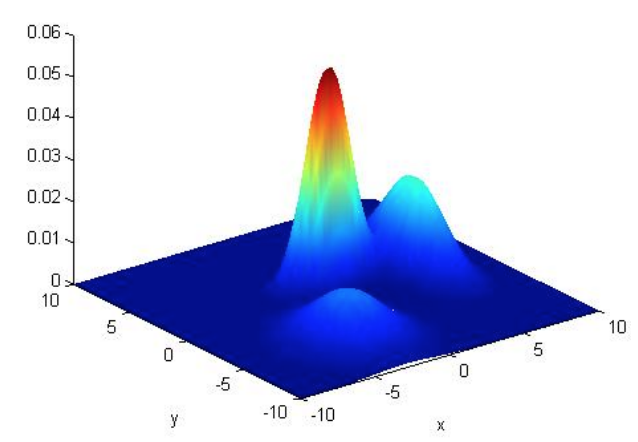
\includegraphics[width=0.85\linewidth]{images/unsupervised/gaussian_mixture/gmm_multivariate.png}
					\caption{GMM applicato su D=2}
				\end{figure}
			\end{columns}
					
%		\end{itemize}
	\end{block}	

\end{frame}


\begin{frame}

	\frametitle{{\color{GradientDescentDiagramOrange}Distribution-based Clustering}: Mixture of Gaussian MultiD}

	\begin{scriptsize}
	\begin{block}{Distribuzione Gaussiana $D = 1$:}
%		\begin{itemize}
			
			\begin{empheq}[box=\fcolorbox{blue!40!black!60}{yellow!10}]{align*}
				\mathcal{N}(x\vert\mu, \sigma)= {\frac{1}{\sigma\sqrt{2\pi}}}e^{- {\frac {1}{2}} (\frac {x-\mu}{\sigma})^2}
			\end{empheq}
			Dove:
			\begin{itemize}
				\item[--] $\mu$ è la media (scalare)
				\item[--] $\sigma$ è la deviazione standard (scalare)
			\end{itemize}
%		\end{itemize}
	\end{block}
	\pause
	\begin{block}{Distribuzione Gaussiana Multivariata $D \geq 1$:}
%		\begin{itemize}
			
			
			\begin{columns}
				\column{0.25\linewidth}
				~
				\column{0.55\linewidth}
				\begin{empheq}[box=\fcolorbox{blue!40!black!60}{yellow!10}]{align*}
					\mathcal{N}(z\vert\mu, C) = (2\pi)^{-\frac{D}{2}} {\vert C\vert}^{-\frac{1}{2}} e^{\frac{-(z-\mu)^T C^{-1} (z-\mu)}{2}}
				\end{empheq}

					
				\column{0.05\linewidth}
				~\\~	\\
				$\rightarrow$
				\column{0.15\linewidth}
				~\\~	\\
				Su R con:  \underline{\href{https://www.rdocumentation.org/packages/LaplacesDemon/versions/16.1.4/topics/dist.Multivariate.Normal}{dmvn}}
			\end{columns}
			
			Dove:
			\begin{itemize}
				\item[--] $z$ è un vettore (vettore colonna $D \times 1$) con le coordinate nello spazio $\mathcal{R}^D$
				\item[--] $\mu$ è il vettore media (vettore colonna $D \times 1$)
				\item[--] $C$ è la matrice di covarianza (matrice $D \times D$)
			\end{itemize}
					
%		\end{itemize}
	\end{block}
	\end{scriptsize}	

\end{frame}



\begin{frame}

	\frametitle{{\color{GradientDescentDiagramOrange}Distribution-based Clustering}: Mixture of Gaussian MultiD}

	\begin{block}{Esempio di normale multivariata con ${\displaystyle {\boldsymbol {\mu }}=\left[{\begin{smallmatrix}0\\0\end{smallmatrix}}\right]}$ and ${\displaystyle {\boldsymbol {\Sigma }}=\left[{\begin{smallmatrix}1&3/5\\3/5&2\end{smallmatrix}}\right]}$}
		\begin{figure}[!htbp]
			\centering
			
			\begin{columns}

				\column{0.5\linewidth}
				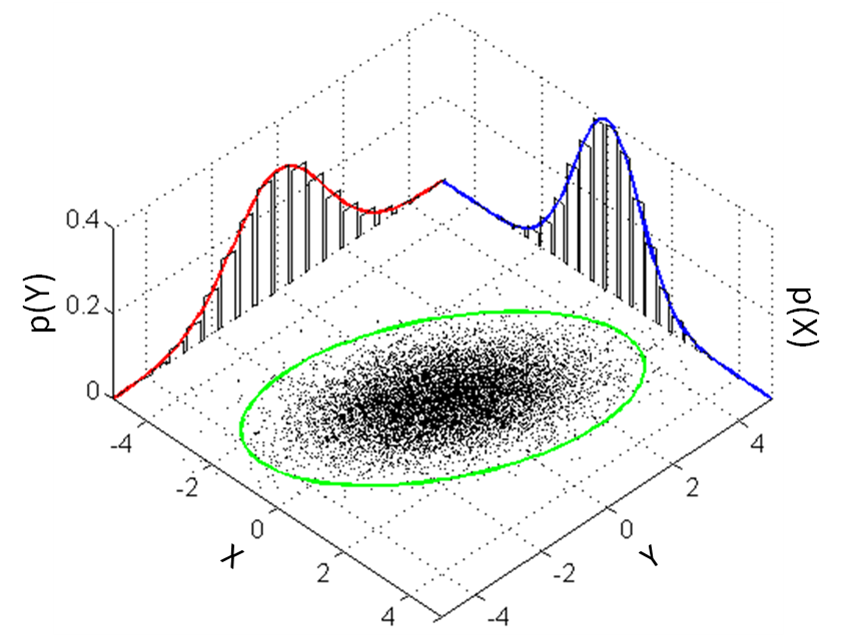
\includegraphics[width=0.8\linewidth]{images/unsupervised/gaussian_mixture/multivariate_normal_1.png}
				\caption{In nero alcuni punti campionati dalla distribuzione, in verde l'ellisse 3-$\sigma$, in blu e rosso le due distribuzioni marginali e i due istogrammi 1-$d$.}
					
				\column{0.5\linewidth}
				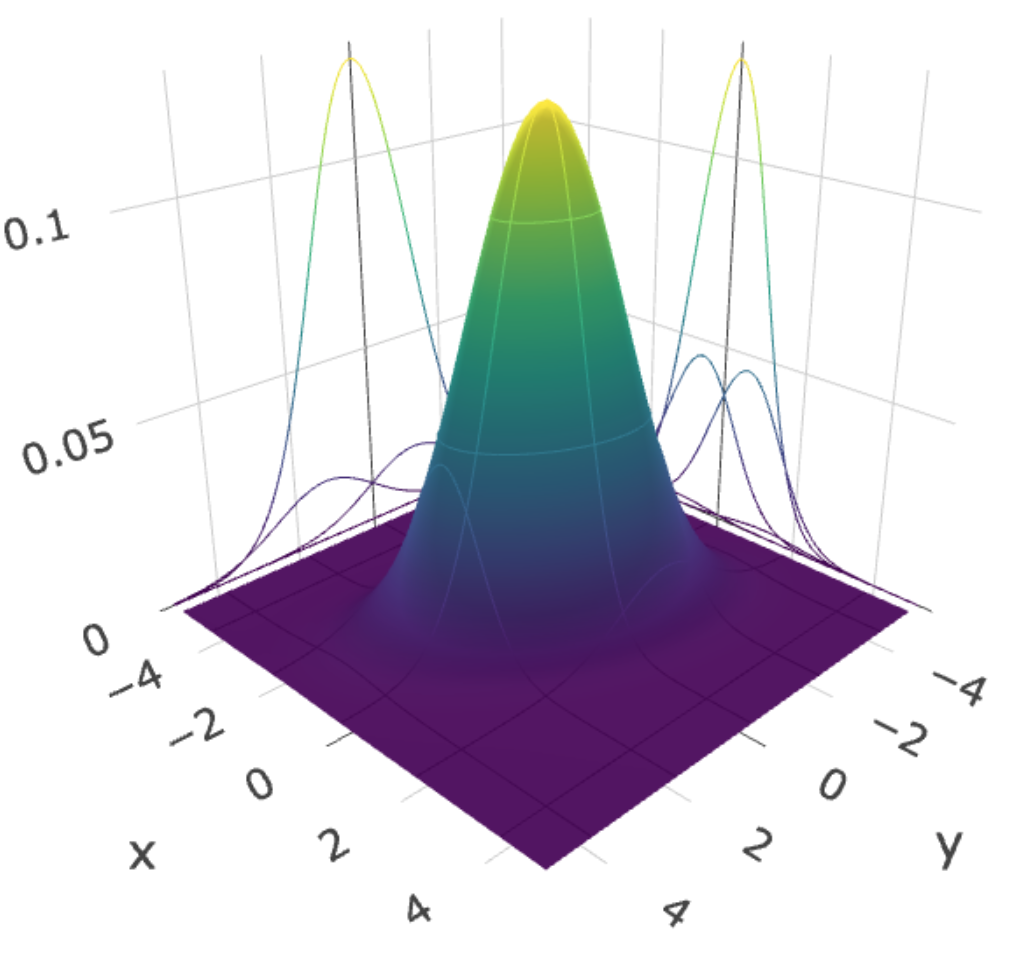
\includegraphics[width=0.85\linewidth]{images/unsupervised/gaussian_mixture/multivariate_normal_2.png}
				\caption{Densità di probabilità.}
			\end{columns}
			
			
		\end{figure}
	\end{block}

\end{frame}

}{}


\begin{frame}

	\frametitle{{\color{GradientDescentDiagramOrange}Distribution-based Clustering}: Mixture of Gaussian}

	%\begin{block}{}
		\begin{itemize}
			\item la densità della distribuzione dei dati in una posizione generica $z$ (vettore colonna) nello spazio delle features $R^D$:
				\begin{empheq}[box=\fcolorbox{blue!40!black!60}{yellow!10}]{align*}
					p(z \vert \Theta )=\sum_{k=1}^{K}\pi_k \mathcal{N}(z\vert\mu_k, C_k)
				\end{empheq}
			\item dove:
				\begin{itemize}
					\item[--] $\Theta = \{ \pi_1, ..., \pi_K, \mu_1, ..., \mu_K, C_1, ..., C_K\}$ è il set dei parametri della mixture di $K$ componenti
					\item[--] $\pi_k$ sono i parametri di mixing per i quali vale:\\
						$\sum\pi_k=1$ e $\pi_k>0$
					\item[--] $\mathcal{N}(z\vert\mu_k, C_k)$ è il valore della $k$-esima Gaussiana multivariata in z:
				\end{itemize}
				
				\begin{empheq}[box=\fcolorbox{blue!40!black!60}{yellow!10}]{align*}
					\mathcal{N}(z\vert\mu_k, C_k) = (2\pi)^{-\frac{D}{2}} {\vert C_k\vert}^{-\frac{1}{2}} e^{\frac{-(z-\mu_k)^T C_{k}^{-1} (z-\mu_k)}{2}}
				\end{empheq}

		\end{itemize}
	%\end{block}

\end{frame}


\begin{frame}

	\frametitle{{\color{GradientDescentDiagramOrange}Distribution-based Clustering}: Mixture of Gaussian}

	%\begin{block}{}
		\begin{empheq}[box=\fcolorbox{blue!40!black!60}{yellow!10}]{align*}
			p(z \vert \Theta )=\sum_{k=1}^{K}\pi_k \mathcal{N}(z\vert\mu_k, C_k)
		\end{empheq}

		\begin{itemize}
			\item i parametri da stimare sono:
				\begin{itemize}
					\item[--] il numero $K$ di clusters
					\item[--] i parametri di mixing $\pi_1,...,\pi_K$ (valori scalari)
					\item[--] i vettori delle medie $\mu_1,...,\mu_K$ (vettori colonna)
					\item[--] le matrici di covarianza $C_1,...,C_K$
				\end{itemize}
			\item rispetto a K-mean, il numero di parametri è maggiore. Pertanto, dovrebbe essere disponibile un numero maggiore di dati
				\begin{itemize}
					\item[--] altrimenti, è molto probabile che si otterrà una stima imprecisa dei valori dei parametri
				\end{itemize}

		\end{itemize}
	%\end{block}

\end{frame}


\begin{frame}

	\frametitle{{\color{GradientDescentDiagramOrange}Distribution-based Clustering}: Gaussian Mixture (GM)}

	%\begin{block}{}


		\begin{itemize}
			\item tipicamente, si presume che il numero $K$ di componenti gaussiane sia noto
			\item i valori degli altri parametri sono stimati tramite l'algoritmo \textbf{Expectation-Maximization}
			\item si tratta di una procedura che aggiorna iterativamente i valori dei parametri attraverso la definizione di una \textbf{hidden ownership variable} $x_{ik}$ (valore scalare):
				\begin{itemize}
					\item[--] $x_{ik}$ rappresenta la probabilità (likelihood) che l'$i$-esimo dato sia generato dal $k$-esimo componente della mixture di gaussiane
				\end{itemize}

		\end{itemize}
	%\end{block}

\end{frame}


\begin{frame}

	\frametitle{{\color{GradientDescentDiagramOrange}Distribution-based Clustering}: EM algorithm for GM}

	%\begin{block}{}
		\begin{enumerate}
			\item inizializzazione randomica dei parametri $\pi_k, \mu_k, C_k$
			\item (\textbf{E}) calcola la \textbf{expectation} delle \textit{ownership variables} $x_{ik}$:
				\begin{scriptsize}
					\begin{empheq}[box=\fcolorbox{blue!40!black!60}{yellow!10}]{align*}
						x_{ik} = \frac{\pi_k \mathcal{N}(z_i\vert\mu_k,C_k)}{\sum_{j=1}^{K}\pi_j \mathcal{N}(z_i\vert\mu_j,C_j)} \qquad \left( \implies \sum_{k=1}^{K}x_{ik} = 1 \right)
					\end{empheq}
				\end{scriptsize}
			\item (\textbf{M}) utilizza le expectation delle \textit{ownership variables} per effettuare una stima della \textbf{massima verosimiglianza} dei parametri $\pi_k, \mu_k, C_k$:
				\begin{scriptsize}
					\begin{empheq}[box=\fcolorbox{blue!40!black!60}{yellow!10}]{align*}
						\pi_k = \frac{1}{N} \sum_{i=1}^{N}x_{ik} \qquad \mu_k = \frac{1}{N\pi_k}\sum_{i=1}^{N}x_{ik}z_i \qquad C_k = \frac{1}{N\pi_k} \sum_{i=1}^{N} x_{ik} (z_i-\mu_k)(z_i-\mu_k)^T
					\end{empheq}
				\end{scriptsize}
			\item Interrompi se la \textbf{log-likelihood} non è cambiata in modo significativo rispetto alla configurazione dell'iterazione precedente (vedi dopo lg-$\ell$).\\
				Altrimenti vai al passaggio 2.
		\end{enumerate}

	%\end{block}

\end{frame}


\begin{frame}

	\frametitle{{\color{GradientDescentDiagramOrange}Distribution-based Clustering}: EM algorithm for GM}

	%\begin{block}{}
		\begin{figure}[!htbp]
			\centering
			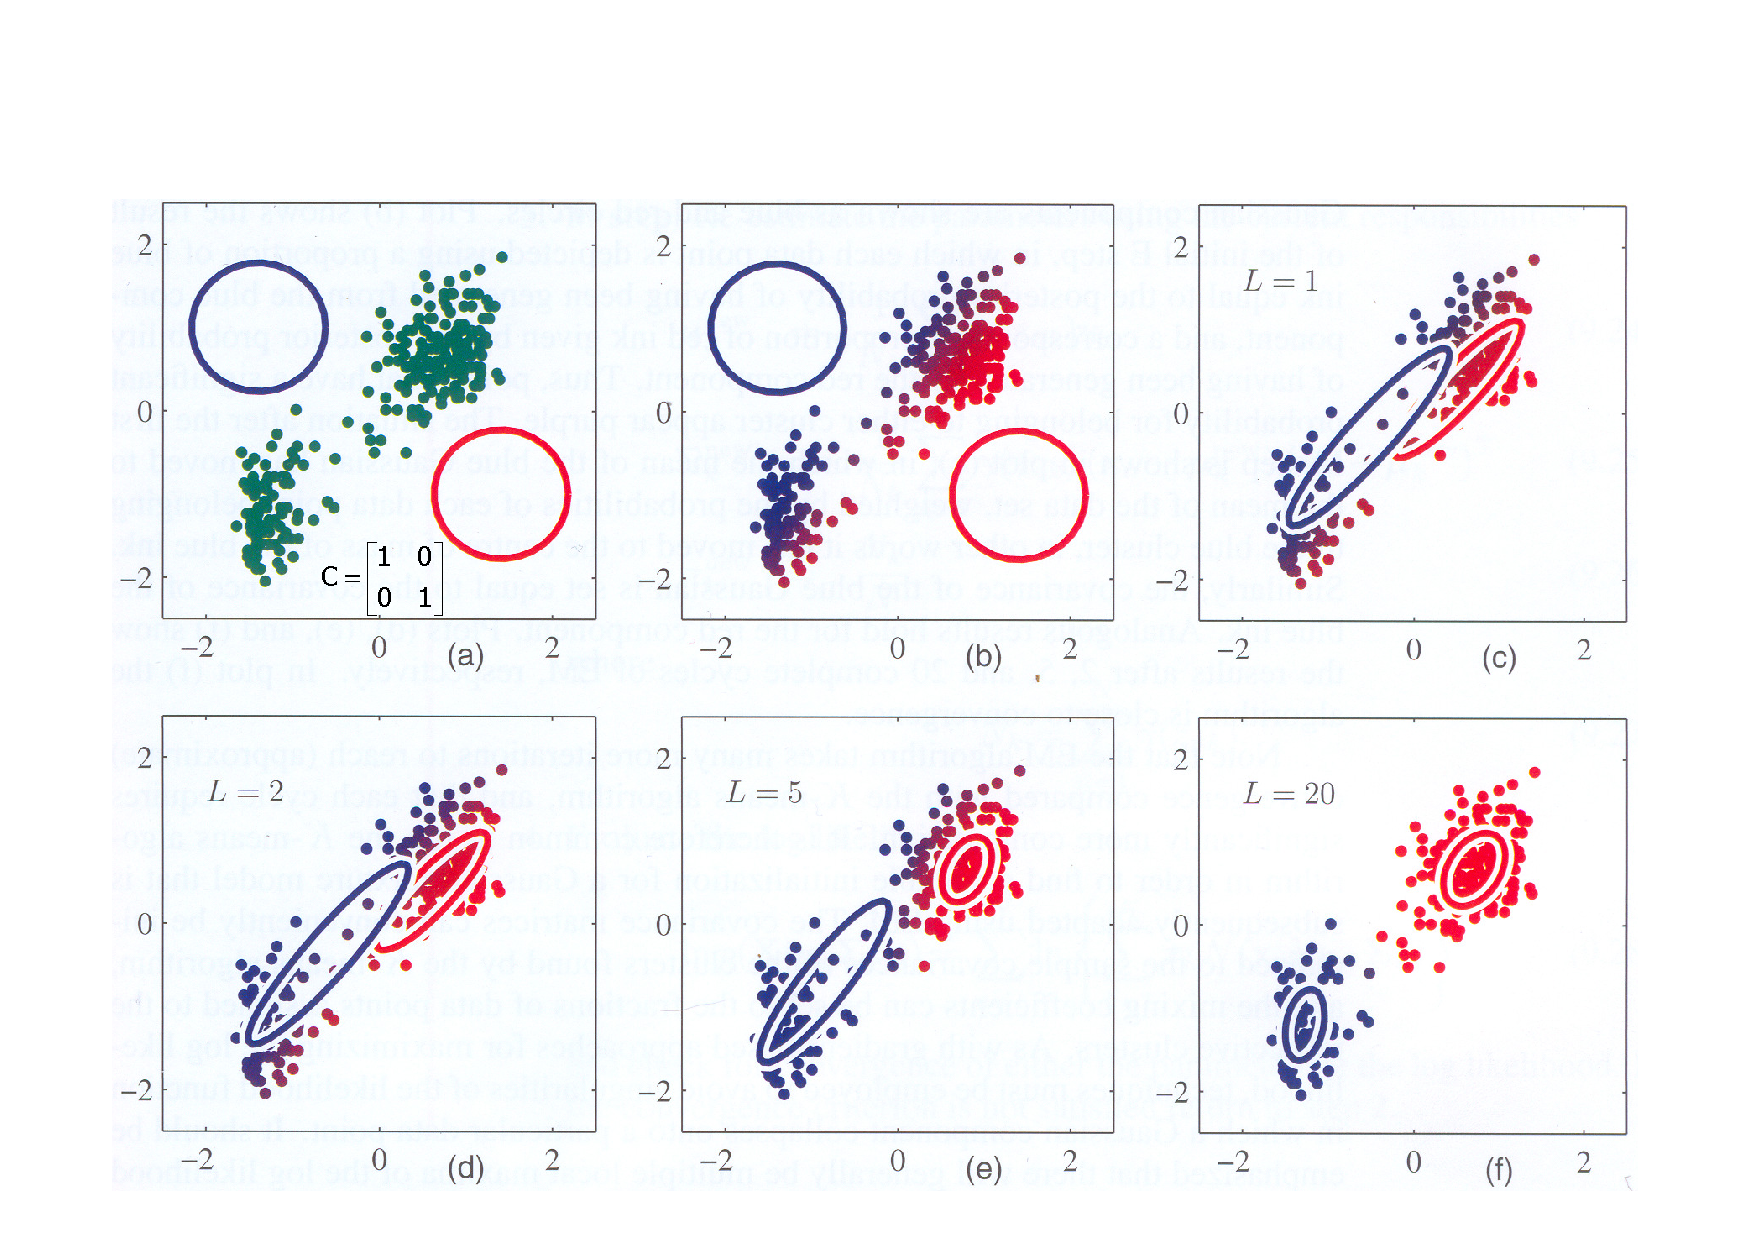
\includegraphics[width=0.9\linewidth]{images/unsupervised/gaussian_mixture/gmm_1.pdf}
					%\caption{Stripe Radar for Fraud Detection}
		\end{figure}
	%\end{block}

\end{frame}


\begin{frame}

	\frametitle{{\color{GradientDescentDiagramOrange}Distribution-based Clustering}: EM algorithm for GM}

		La convergenza viene generalmente rilevata calcolando il valore della \textbf{log-likelihood} dopo ogni iterazione e interrompendosi quando sembra non cambiare in modo significativo da un'iterazione alla successiva.\\
		Si noti che la log-likelihood (nell'ipotesi IID) è definita come segue:
		\begin{empheq}[box=\fcolorbox{blue!40!black!60}{yellow!10}]{align*}
			log\text{ }\ell (\Theta) = \sum_{i=1}^{N} log\text{ }p(z_i \vert \Theta) = \sum_{i=1}^{N} \left( log \sum_{k=1}^{K} \pi_k \mathcal{N}(z_i\vert\mu_k,C_k) \right)
		\end{empheq}

		Dove:
		\begin{itemize}
			\item[--] $z_i$ è la $i$-esima istanza del dataset
			\item[--] $K$ è il numero di clusters
			\item[--] $\pi_1,...,\pi_K$ sono i parametri di mixing (valori scalari)
			\item[--] $\mu_1,...,\mu_K$ sono i vettori delle medie (vettori colonna)
			\item[--] $C_1,...,C_K$ sono le matrici di covarianza 
		\end{itemize}
		
\end{frame}


\begin{frame}

	\frametitle{{\color{GradientDescentDiagramOrange}Distribution-based Clustering}: EM algorithm for GM}	\centering
		\animategraphics[controls={play, step, stop}, height=7cm]{7.0}{images/unsupervised/gaussian_mixture/em_for_gm/em_for_gm-}{0}{49}
\end{frame}


\begin{frame}

	\frametitle{{\color{GradientDescentDiagramOrange}Distribution-based Clustering}: EM algorithm for GM}
	%\begin{block}{}
		\begin{figure}[!htbp]
			\centering
			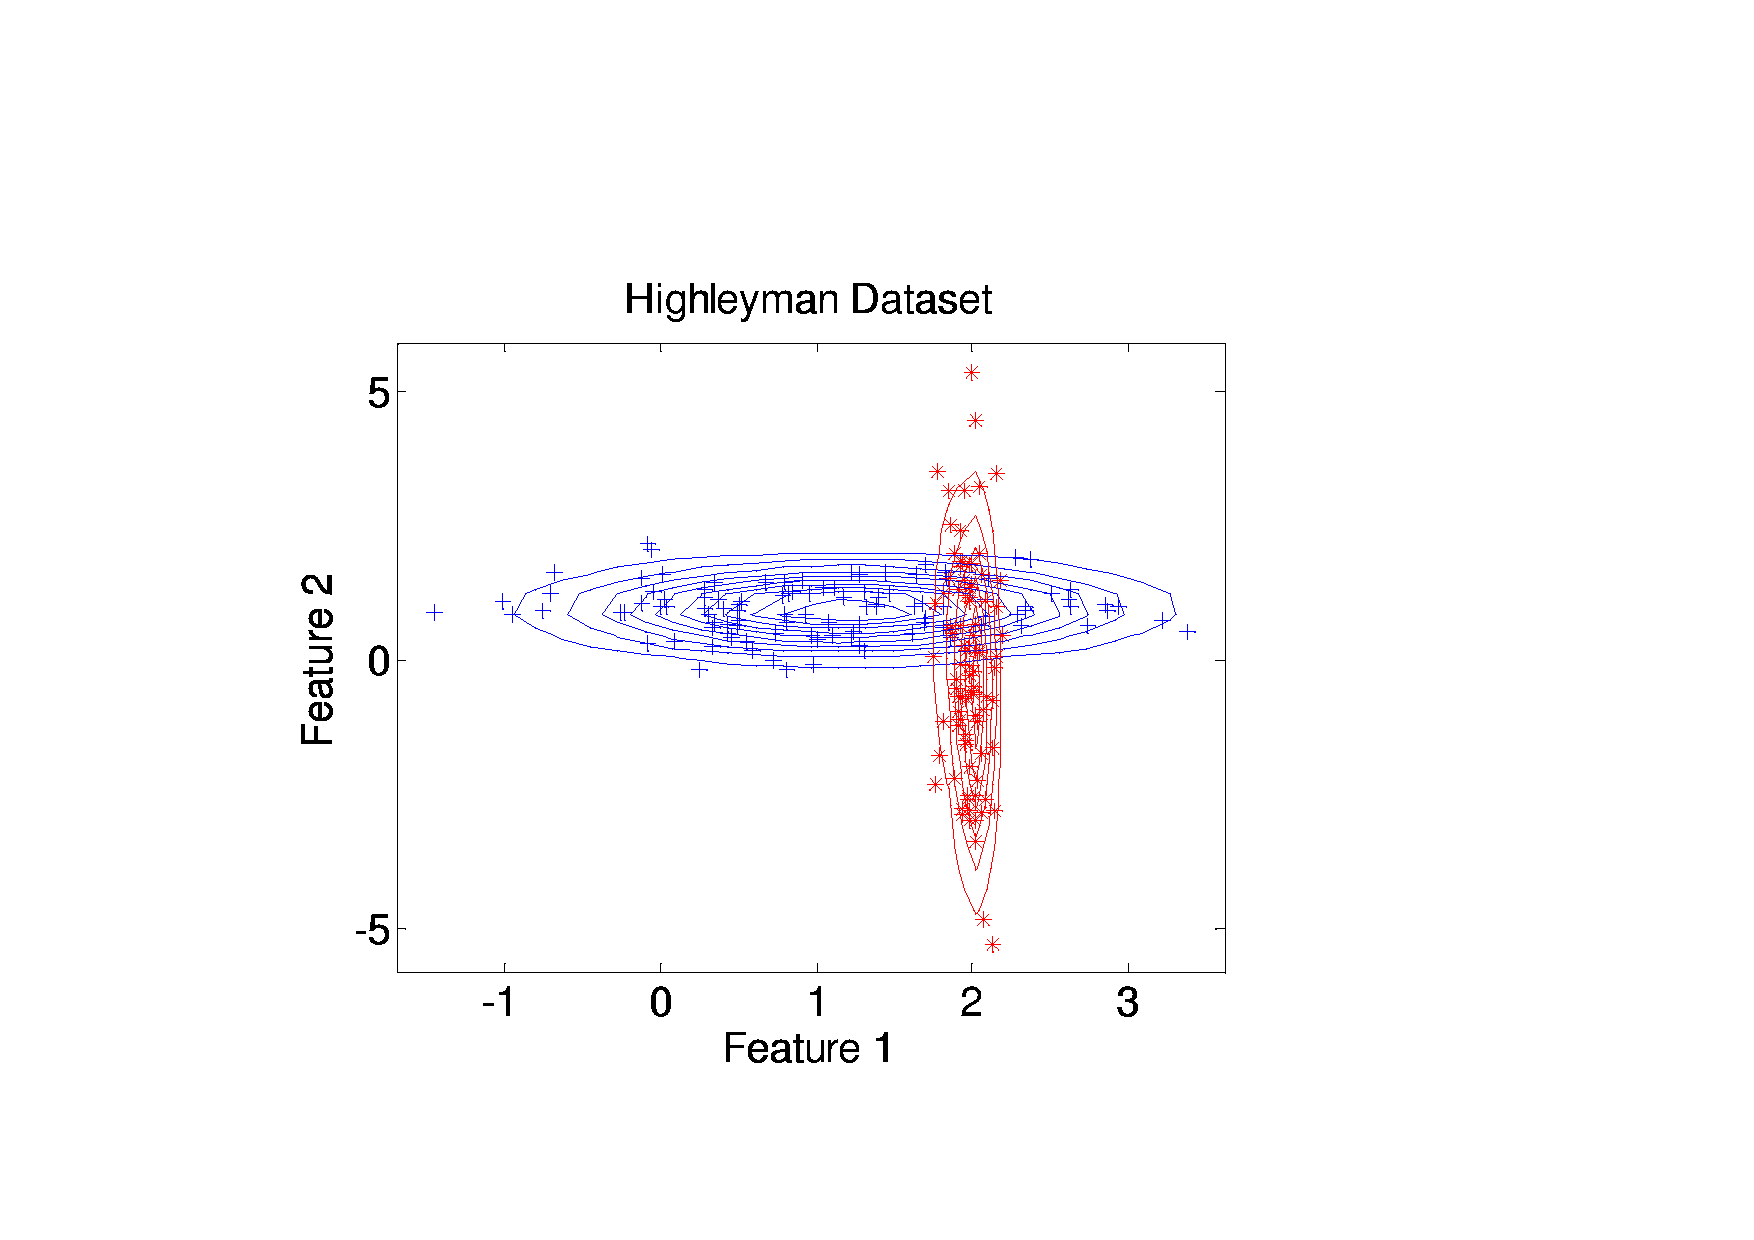
\includegraphics[width=0.6\linewidth]{images/unsupervised/gaussian_mixture/gmm_2.pdf}
					%\caption{Stripe Radar for Fraud Detection}
		\end{figure}
	%\end{block}

\end{frame}


\begin{frame}

	\frametitle{{\color{GradientDescentDiagramOrange}Distribution-based Clustering}: EM algorithm for GM}

	%\begin{block}{}
		\begin{itemize}
			\item la stima dei valori dei parametri potrebbe non essere accurata se il numero dei punti del dataset è basso
		\end{itemize}
		\begin{figure}[!htbp]
			\centering
			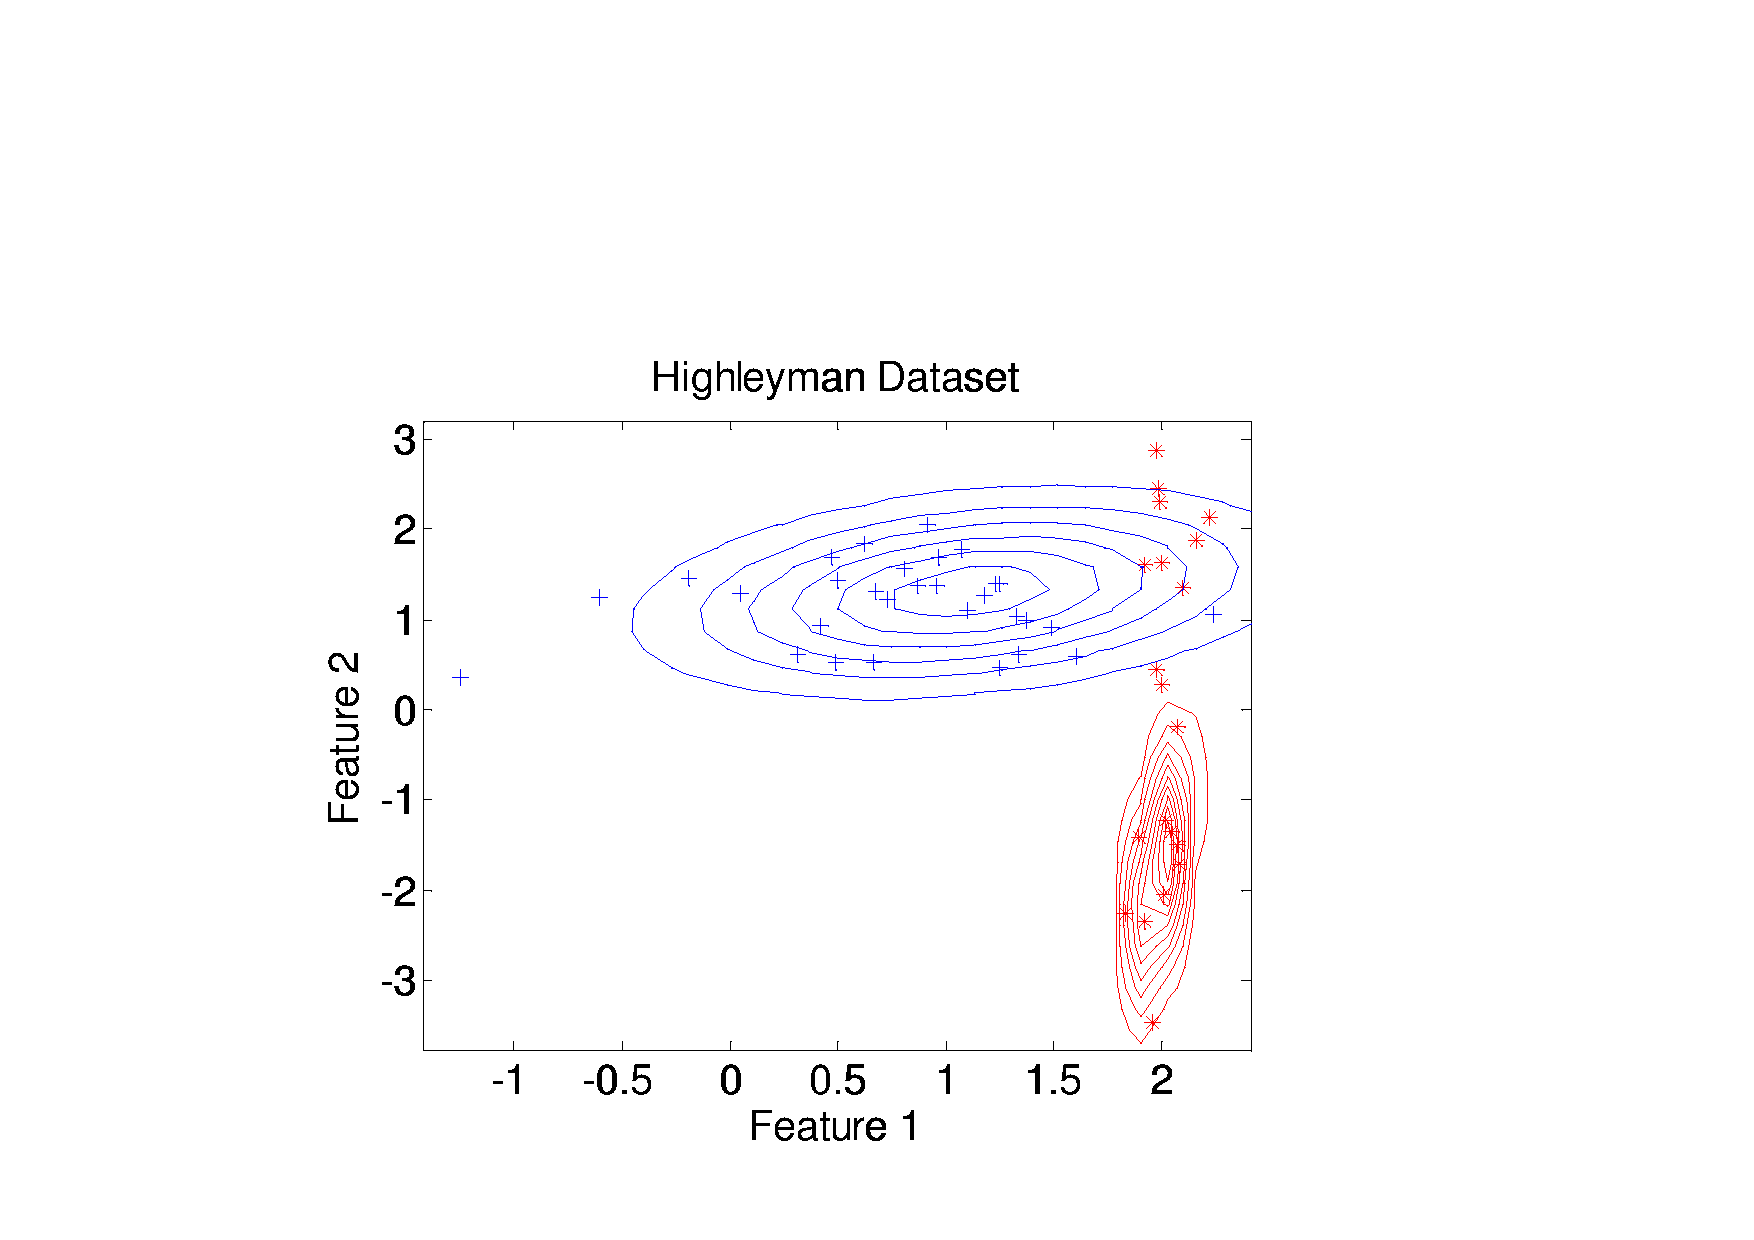
\includegraphics[width=0.6\linewidth]{images/unsupervised/gaussian_mixture/gmm_3.pdf}
					%\caption{Stripe Radar for Fraud Detection}
		\end{figure}
	%\end{block}

\end{frame}


\begin{frame}

	\frametitle{{\color{GradientDescentDiagramOrange}Distribution-based Clustering}: EM algorithm for GM}

	%\begin{block}{}
		\begin{itemize}
			\item Una volta determinati i parametri della mistura gaussiana, la segmentazione si ottiene assegnando l'$i$-esima istanza al cluster con il valore massimo della \textit{ownership variable} $x_{ik}$:
			\begin{empheq}[box=\fcolorbox{blue!40!black!60}{yellow!10}]{align*}
				x_{ik} = \frac{\pi_k \mathcal{N}(z_i\vert\mu_k,C_k)}{\sum_{j=1}^{K}\pi_j \mathcal{N}(z_i\vert\mu_j,C_j)}
			\end{empheq}
		\end{itemize}
	%\end{block}

\end{frame}


\begin{frame}

	\frametitle{{\color{GradientDescentDiagramOrange}Distribution-based Clustering}: segmentazione con il GMM}

%	\begin{block}{K-means: considerazioni}
		\begin{figure}[!htbp]
				\centering
				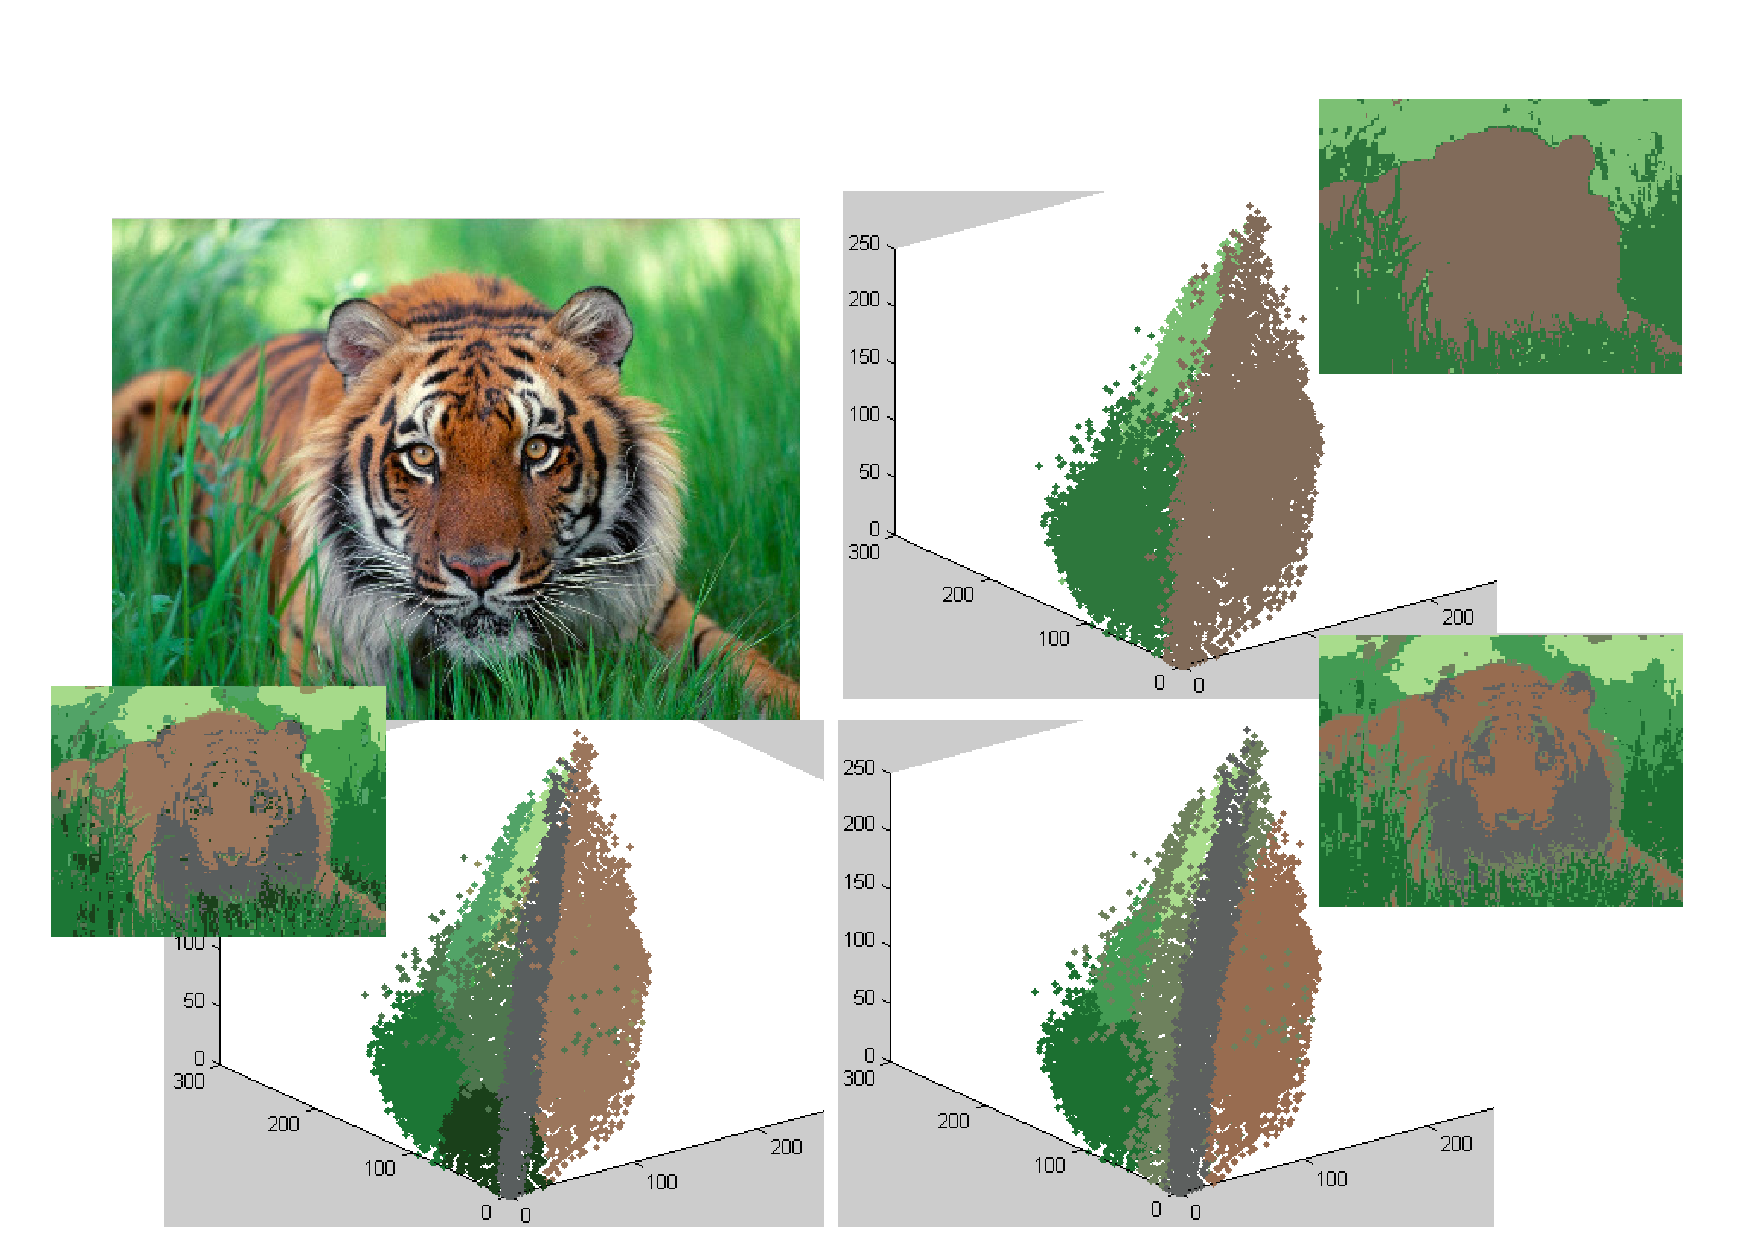
\includegraphics[angle=0,width=0.85\linewidth]{images/unsupervised/gaussian_mixture/gmm_lion.pdf}
%				\caption{Single-Link Dendogram Good K}
				%\label{Enel_QQ_Plot_Normal}
			\end{figure}
%	\end{block}

\end{frame}


\begin{frame}

	\frametitle{{\color{GradientDescentDiagramOrange}Distribution-based Clustering}: segmentazione con il GMM}

%	\begin{block}{K-means: considerazioni}
		\begin{figure}[!htbp]
				\centering
				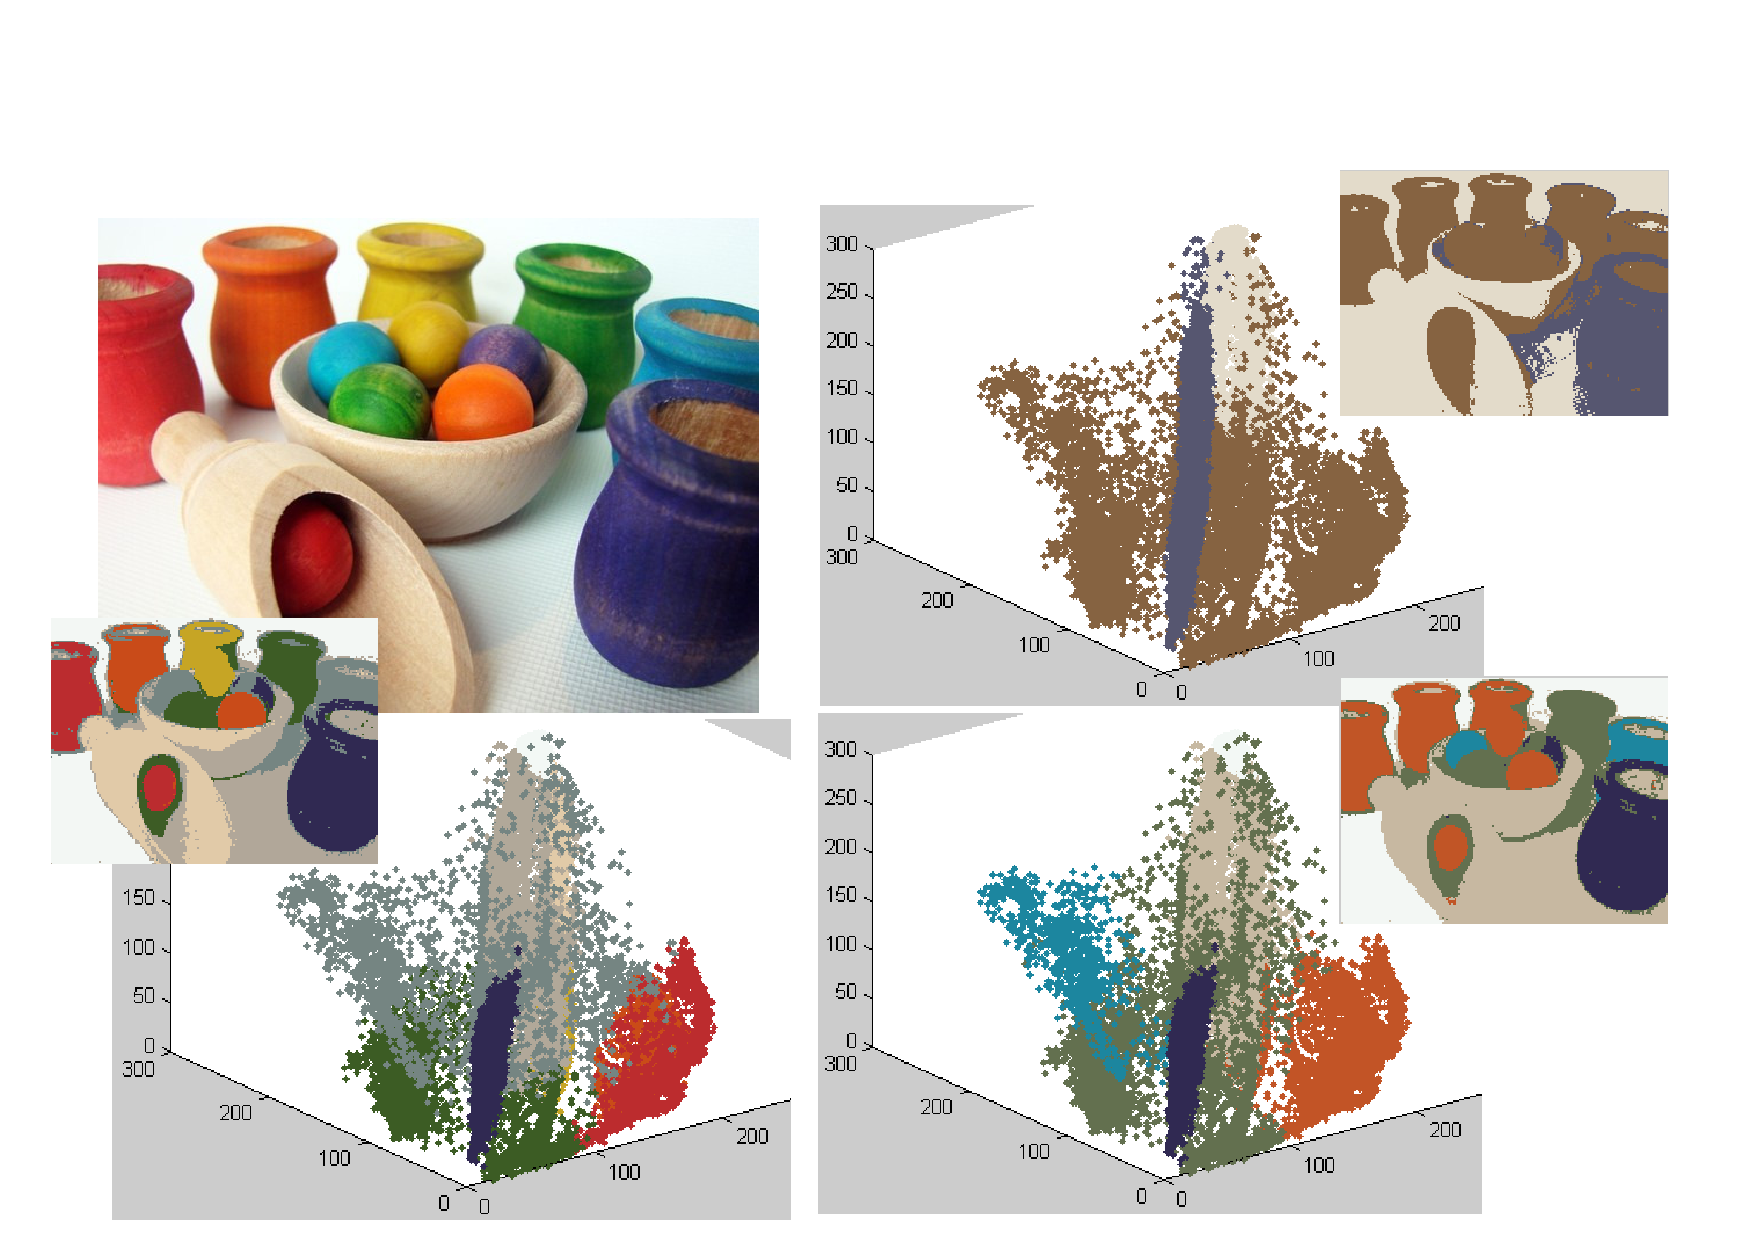
\includegraphics[angle=0,width=0.9\linewidth]{images/unsupervised/gaussian_mixture/gmm_pots.pdf}
%				\caption{Single-Link Dendogram Good K}
				%\label{Enel_QQ_Plot_Normal}
			\end{figure}
%	\end{block}

\end{frame}


\begin{frame}

	\frametitle{{\color{GradientDescentDiagramOrange}Distribution-based Clustering}: limiti del GMM}

%	\begin{block}{K-means: considerazioni}
		\begin{itemize}
			\item inizializzazioni con parametri diversi può portare a differenti risultati
				\begin{itemize}
					\item[--] in effetti, la procedura iterativa per la stima dei parametri può fermarsi in minimi locali della funzione obiettivo
				\end{itemize}
			\item  il numero di componenti della mistura deve essere scelto in partenza
			\item poiché devono essere stimati molti parametri, è richiesto un dataset molto ampio rispetto a quanto necessario con K-means
			\item nessuna garanzia generale che la distribuzione dei dati all'interno di ciascun cluster sia gaussiana
		\end{itemize}
%	\end{block}

\end{frame}


\begin{frame}

	\frametitle{{\color{GradientDescentDiagramOrange}Distribution-based Clustering}: confronto con altre tecniche}

%	\begin{block}{K-means: considerazioni}
		\begin{figure}[!htbp]
				\centering
				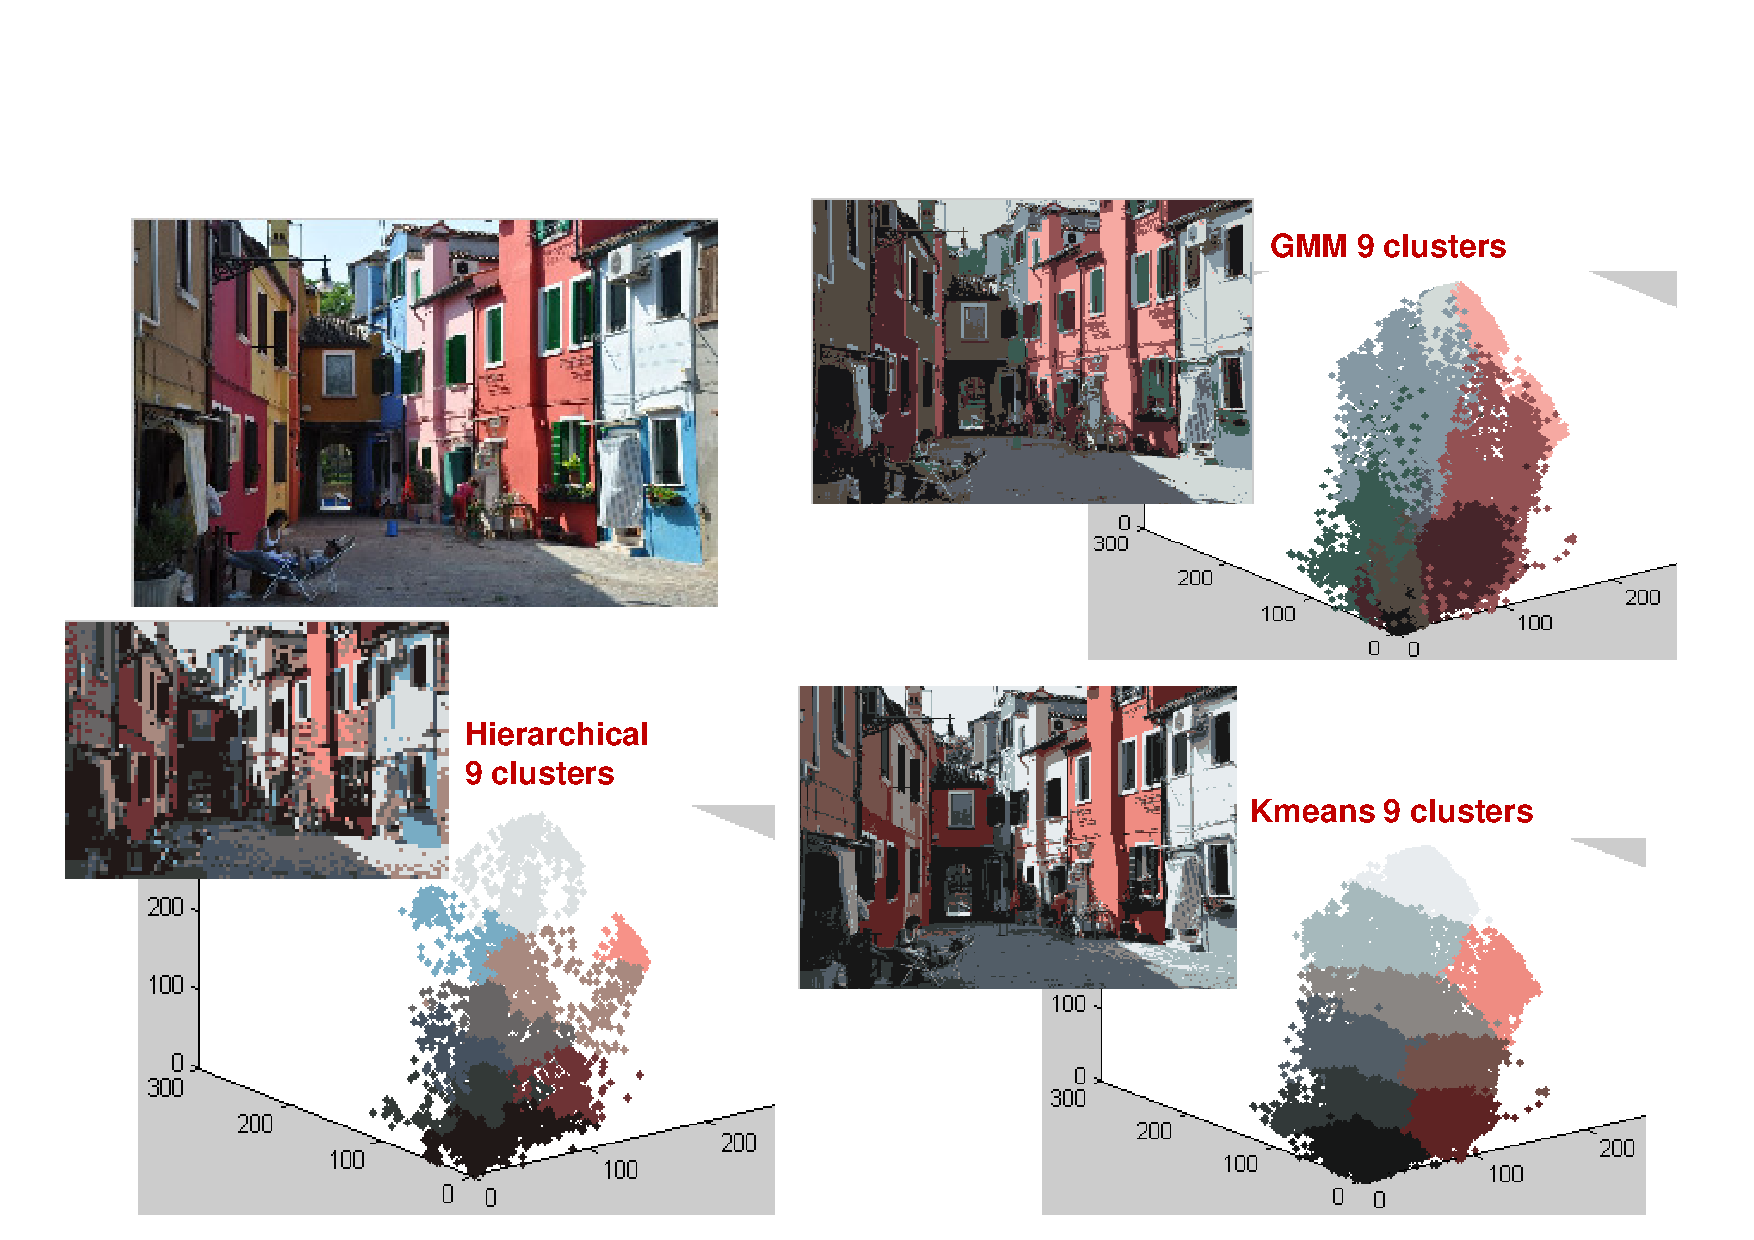
\includegraphics[angle=0,width=0.9\linewidth]{images/unsupervised/gaussian_mixture/hierarchical_vs_kmeans_vs_gmm.pdf}
%				\caption{Single-Link Dendogram Good K}
				%\label{Enel_QQ_Plot_Normal}
			\end{figure}
%	\end{block}

\end{frame}

\ifthenelse{\boolean{highschool}}{}{

\subsubsection[Density-based (Mean shift)]{Density-based \textit{(Mean shift)}}
\begin{frame}

	\frametitle{{\color{GradientDescentDiagramRed}Density-based Clustering}, in sintesi}

	%\begin{block}{}
		Il density-based clustering collega aree ad alta densità in cluster. Ciò consente distribuzioni di forma arbitraria purché sia possibile collegare aree dense.
		\newlinedouble
		Questi algoritmi hanno difficoltà con dati a densità variabile e dimensionalità elevate. Inoltre, per costruzione, questi algoritmi non riescono ad assegnare dei valori anomali ai cluster.
		\begin{figure}[!htbp]
			\centering
			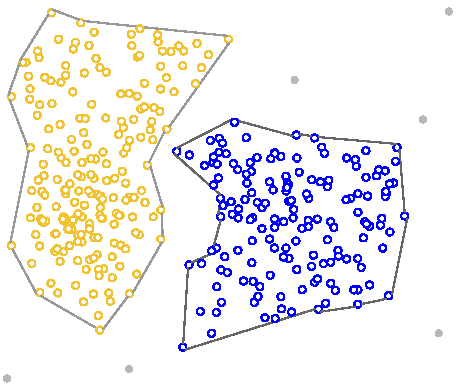
\includegraphics[width=5.0cm]{images/unsupervised/types/Clustering_Density.pdf}
					%\caption{Stripe Radar for Fraud Detection}
		\end{figure}
	%\end{block}

\end{frame}


\begin{frame}

	\frametitle{{\color{GradientDescentDiagramRed}Density-based Clustering}}

	%\begin{block}{}
		\begin{itemize}
			\item gli spazi delle features strutturati arbitrariamente dovrebbero essere analizzati solo attraverso metodi non parametrici che non hanno presupposti incorporati (l'adattamento della distribuzione in figura con un GMM fallirebbe)
		\end{itemize}

		\begin{columns}

			\column{0.5\linewidth}
			\begin{figure}[!htbp]
				\centering
				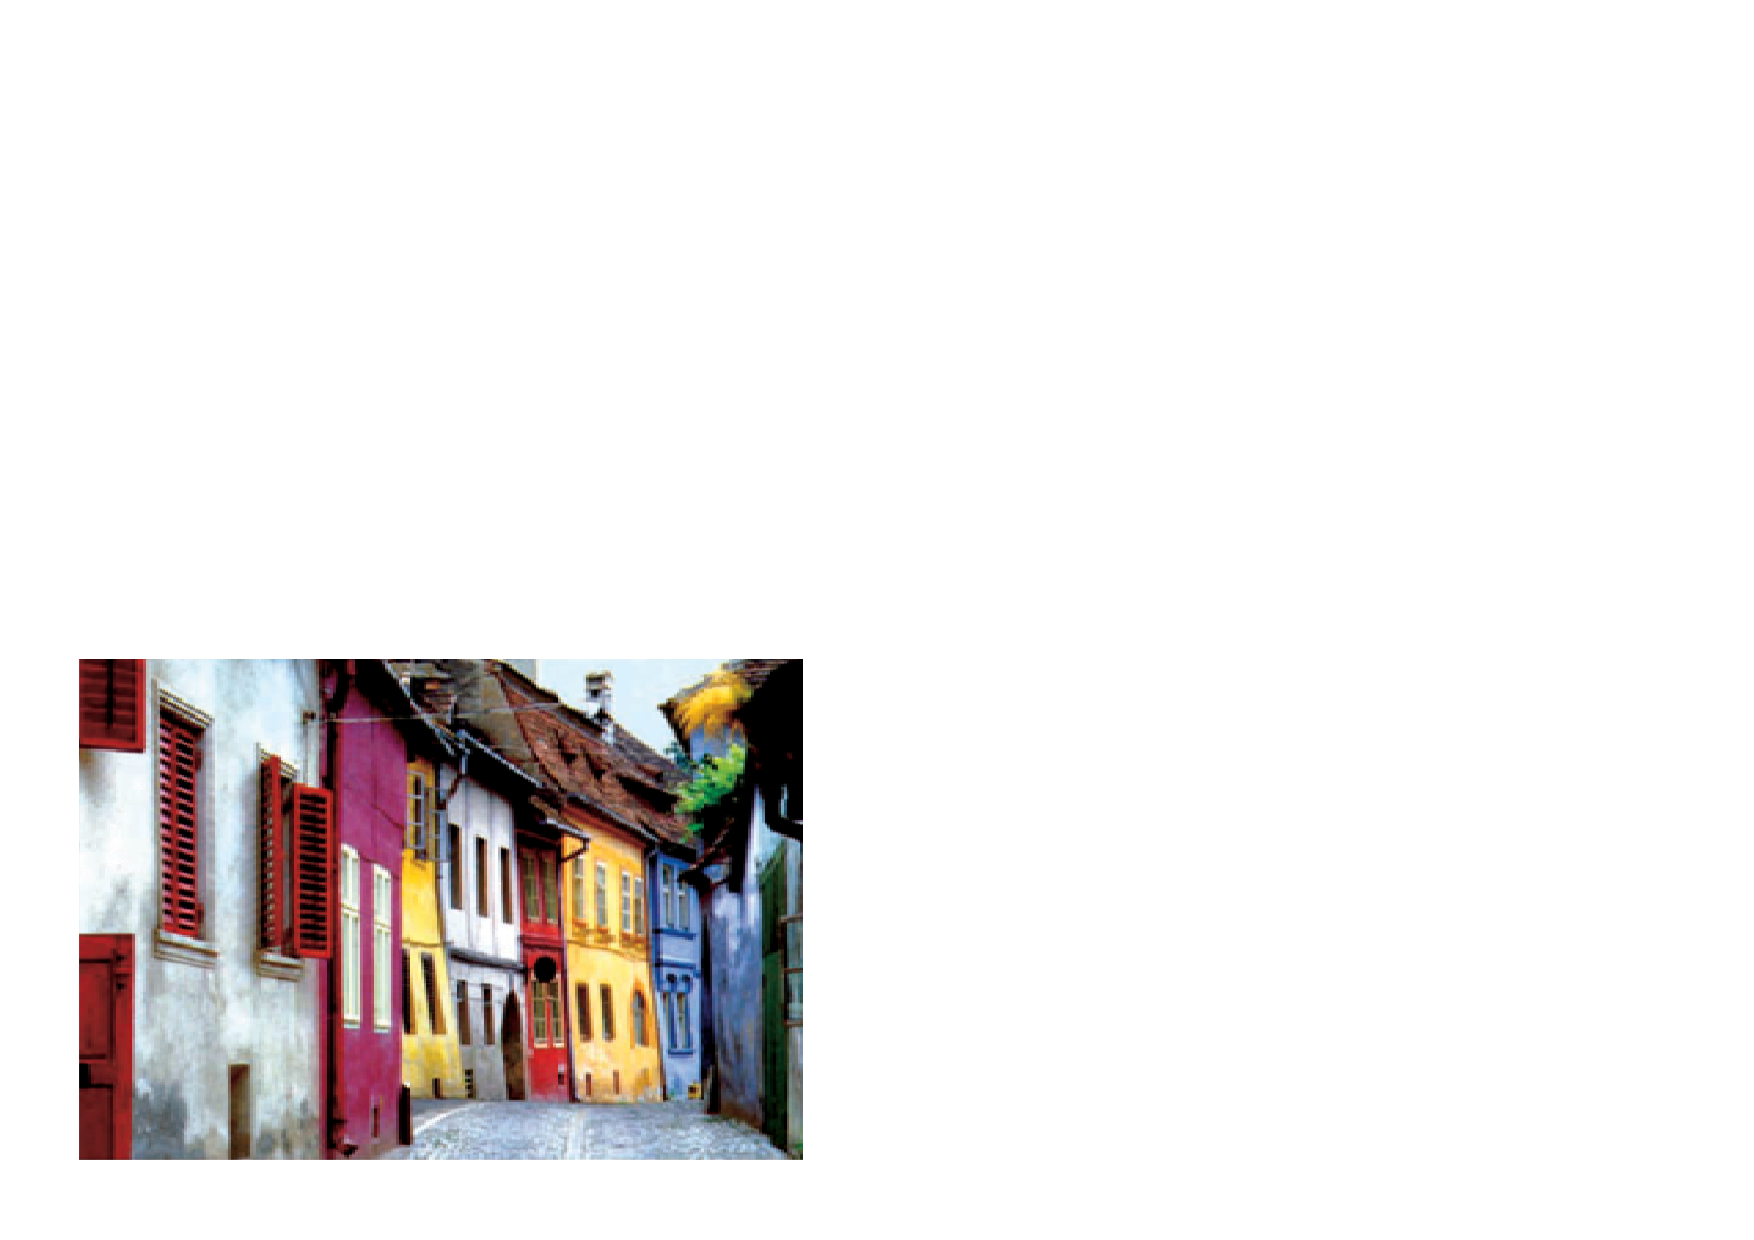
\includegraphics[width=1.0\linewidth]{images/unsupervised/non_parametric/np_1.pdf}
				%\caption{ENEL QQ-Plot Normale}
				%\label{Enel_QQ_Plot_Normal}
			\end{figure}

			\column{0.5\linewidth}
			\begin{figure}[!htbp]
				\centering
				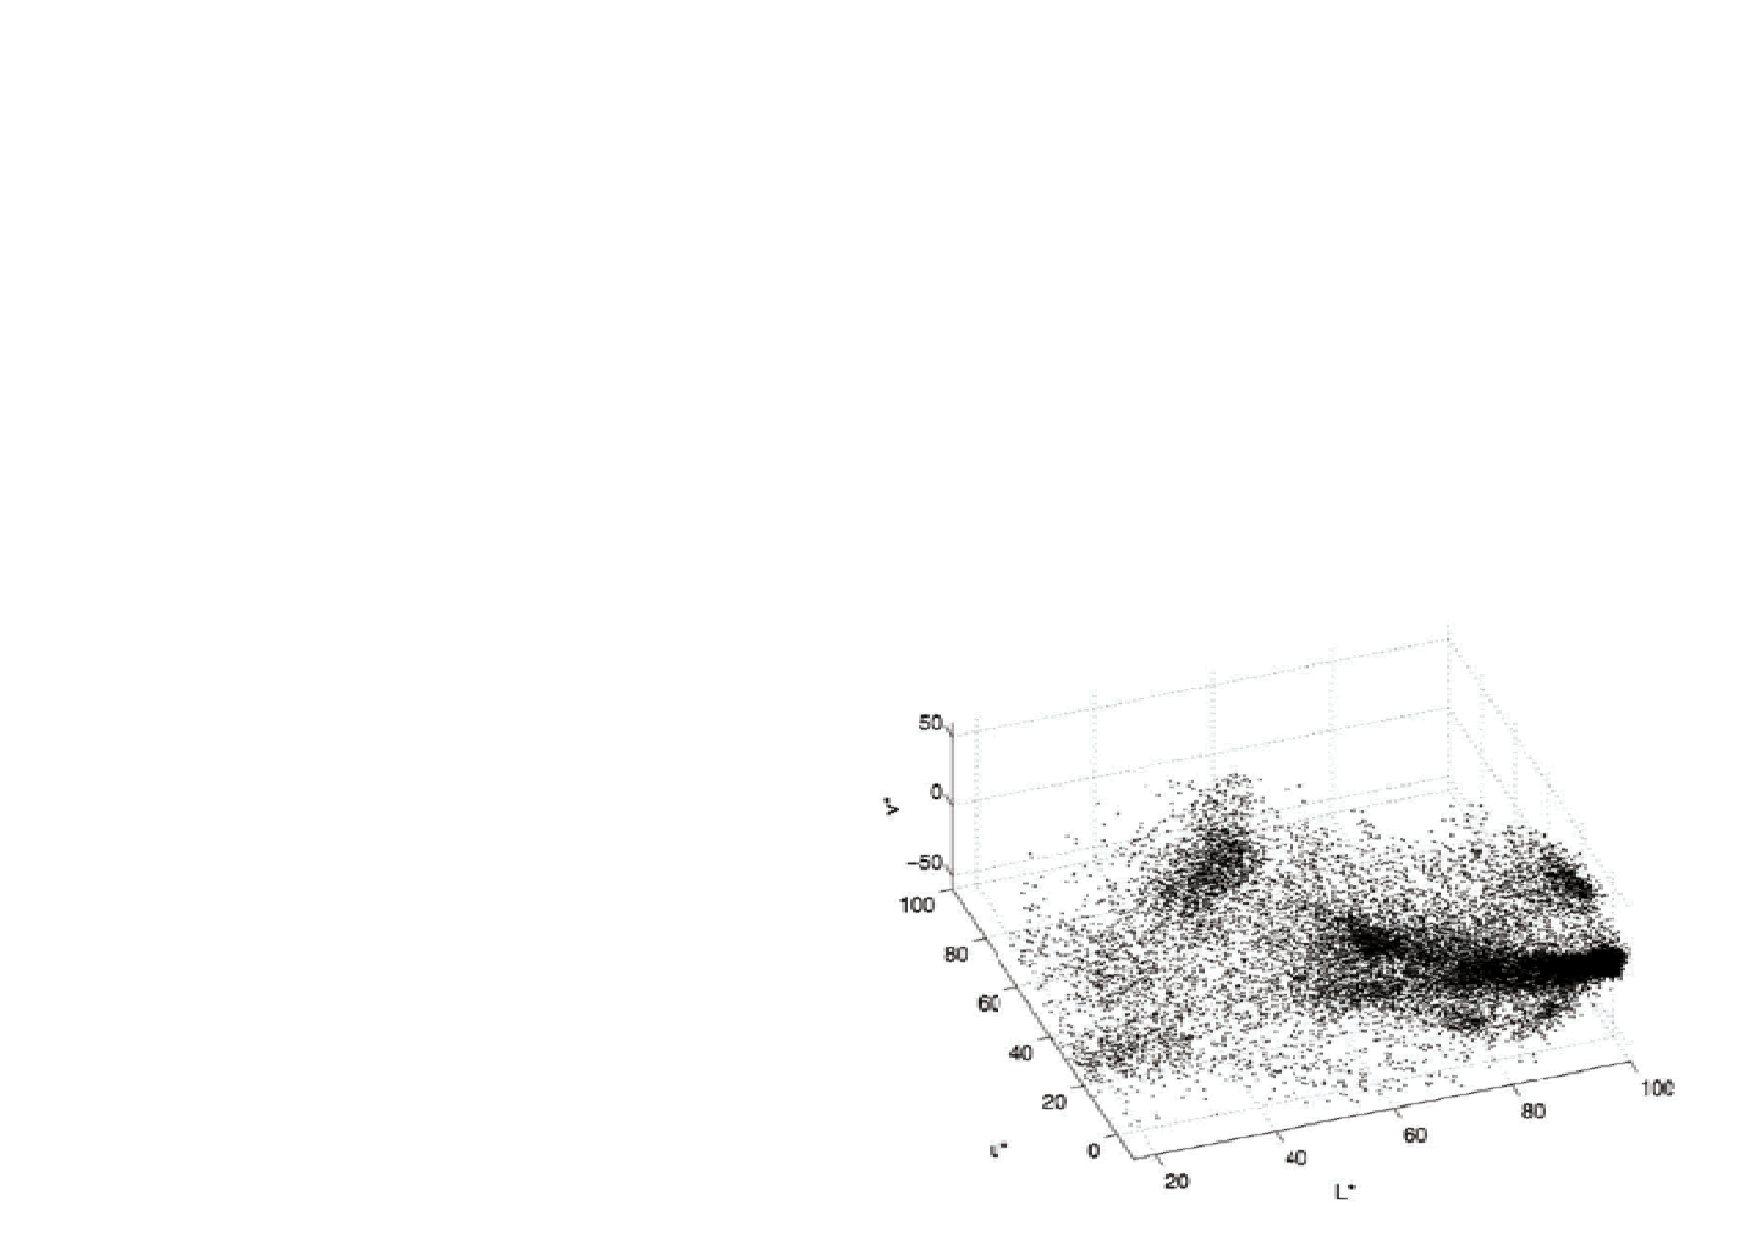
\includegraphics[width=1.0\linewidth]{images/unsupervised/non_parametric/np_2.pdf}
				%\caption{ENEL QQ-Plot Normale}
				%\label{Enel_QQ_Plot_Normal}
			\end{figure}

		\end{columns}

	%\end{block}

\end{frame}


\begin{frame}

	\frametitle{{\color{GradientDescentDiagramRed}Density-based Clustering}}

	%\begin{block}{}
		\begin{itemize}
			\item tutte le soluzioni proposte finora suggeriscono che i centri dei cluster dovrebbero essere localizzati in corrispondenza di regioni dense nello spazio delle caratteristiche
			\item al contrario, le regioni con valori di bassa densità dovrebbero essere considerate come regioni marginali
			\item i \textbf{gaussian mixture models (GMM)} rappresentano una soluzione per stimare i valori della densità attraverso un approccio  \textbf{parametrico, basato su un modello}
			\item tuttavia, il modello gaussiano non è adeguato per rappresentare i valori di densità per distribuzioni di dati generici
		\end{itemize}
	%\end{block}

\end{frame}


\begin{frame}

	\frametitle{{\color{GradientDescentDiagramRed}Density-based Clustering}}

	%\begin{block}{}

		\begin{columns}

			\column{0.67\linewidth}
			\begin{itemize}
				\item un miglioramento rispetto al clustering parametrico basato su modelli è rappresentato da \textbf{approcci di clustering non parametrici}
				\item questi operano una stima della densità nello spazio delle features senza assumere alcun modello di distribuzione specifico
					\begin{itemize}
						\item[--] una volta stimata la densità, vengono rilevati i massimi locali della funzione di densità (i massimi locali sono le \textbf{mode della distribuzione})
						\item[--] ciascuna moda è associata a una regione di influenza nello spazio delle features.\\
							La forma e l'estensione di questa regione è definita dalla forma locale della funzione di densità, non da modelli predefiniti (es. Gaussiani)
					\end{itemize}
			\end{itemize}
			\column{0.33\linewidth}
			\begin{figure}[!htbp]
				\centering
				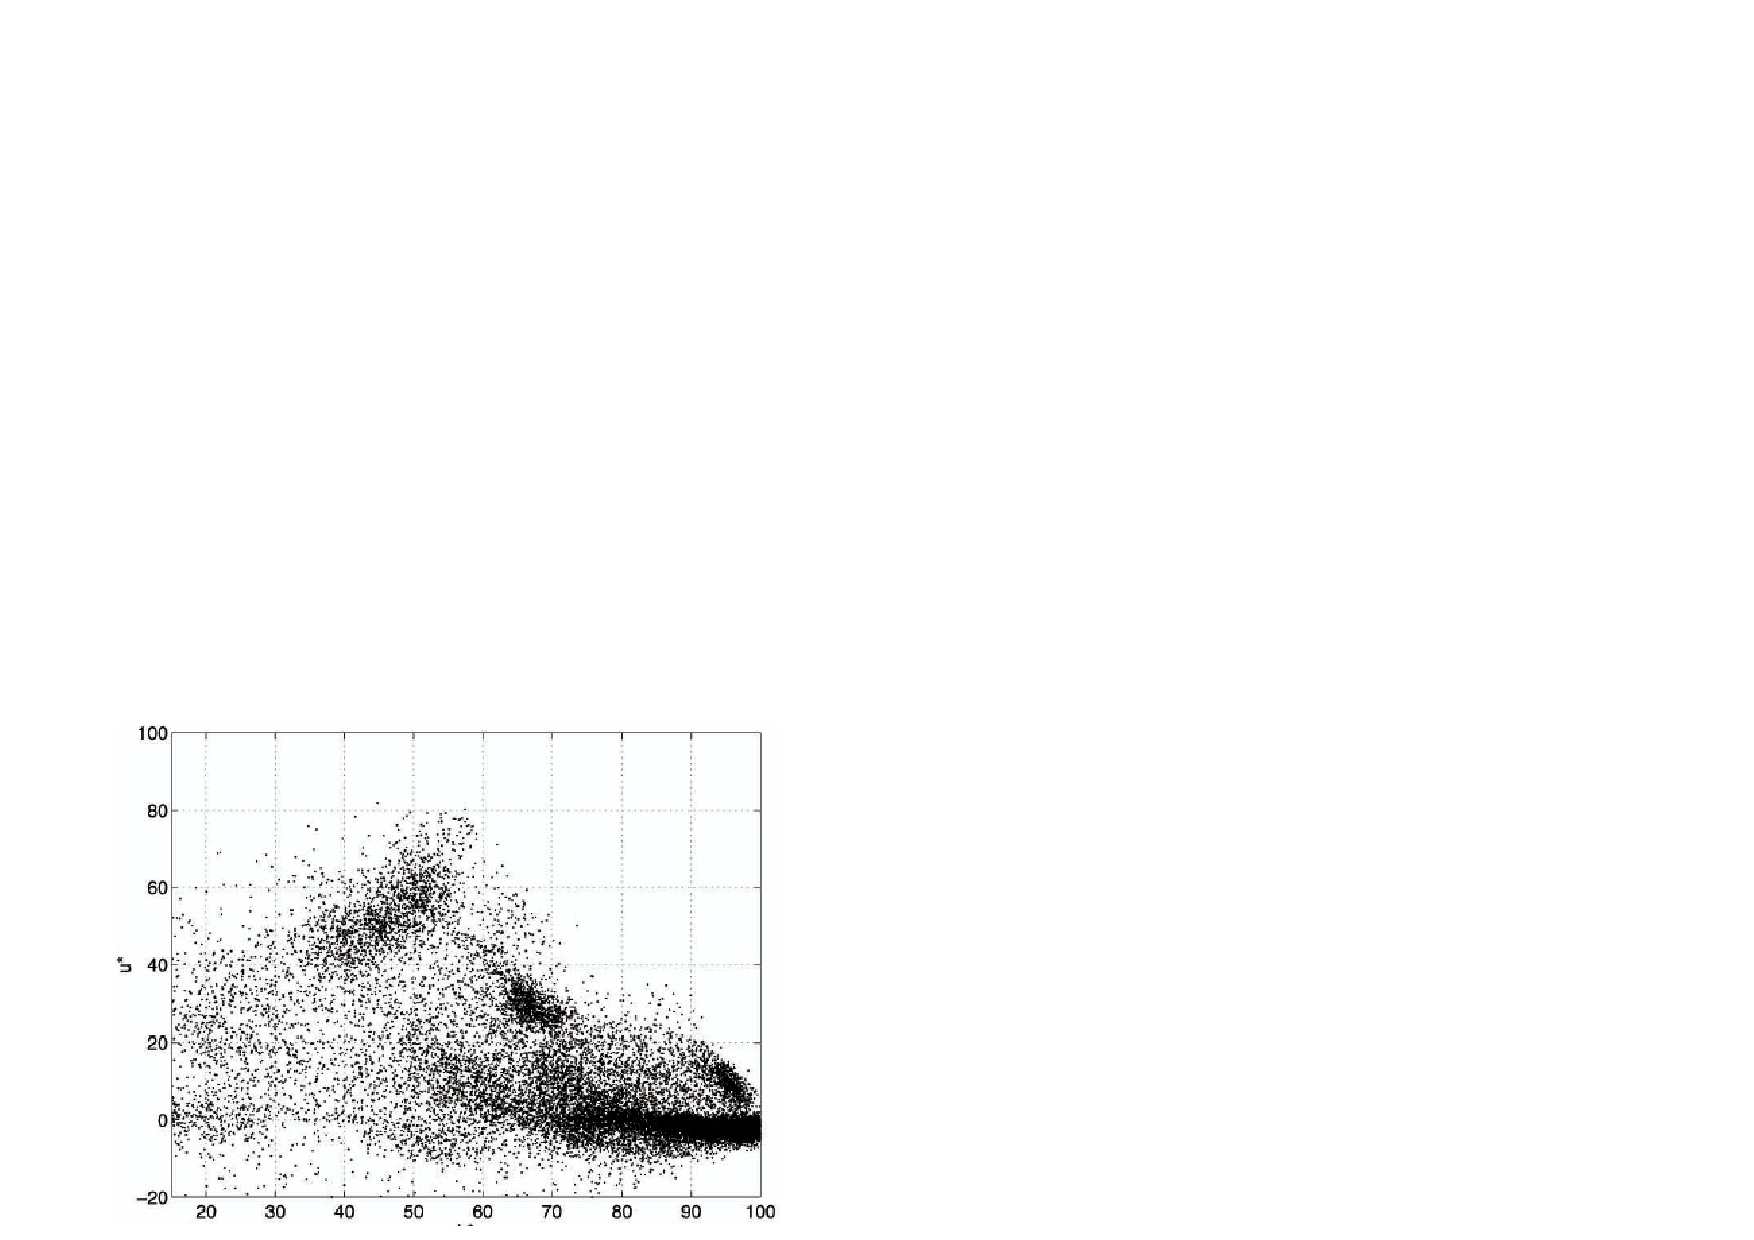
\includegraphics[width=1\linewidth]{images/unsupervised/non_parametric/density.pdf}
				\newlinedouble
				\includegraphics[width=1\linewidth]{images/unsupervised/non_parametric/density_level_curve.pdf}
				%\caption{ENEL QQ-Plot Normale}
				%\label{Enel_QQ_Plot_Normal}
			\end{figure}

		\end{columns}

	%\end{block}

\end{frame}


\begin{frame}

	\frametitle{{\color{GradientDescentDiagramRed}Density-based Clustering}}

	%\begin{block}{}
		\begin{itemize}
%			\item in particolare, la regione di influenza di una  generica moda $q$:\\
%				comprende tutti i punti $p$ sulla superficie della funzione di densità tali che seguendo il percorso che parte da $p$ si fermano in $q$ avendo utilizzato come guida la direzione indicata del gradiente
			\item in particolare, la regione di influenza di una generica moda $q$ comprende tutti i punti $p$ sulla superficie della funzione densità tali che il percorso che parte da $p$ e segue il gradiente della superficie si ferma in $q$
		\end{itemize}

		\begin{columns}

			\column{0.5\linewidth}
			\begin{figure}[!htbp]
				\centering
				\includegraphics[width=0.85\linewidth]{images/unsupervised/non_parametric/density_red.pdf}
				%\caption{ENEL QQ-Plot Normale}
				%\label{Enel_QQ_Plot_Normal}
			\end{figure}

			\column{0.5\linewidth}
			\begin{figure}[!htbp]
				\centering
				\includegraphics[width=1.0\linewidth]{images/unsupervised/non_parametric/density_level_curve.pdf}
				%\caption{ENEL QQ-Plot Normale}
				%\label{Enel_QQ_Plot_Normal}
			\end{figure}

		\end{columns}

	%\end{block}

\end{frame}


\begin{frame}

	\frametitle{{\color{GradientDescentDiagramRed}Density-based Clustering}}

	%\begin{block}{}

		\begin{itemize}
			\item la segmentazione dell'immagine si ottiene:
				\begin{itemize}
					\item[--] associando ogni punto nello spazio delle features con la moda della regione di influenza a cui appartiene il punto
					\item[--] proiettando le regioni di influenza sull'immagine originale
				\end{itemize}
		\end{itemize}

		\begin{figure}[!htbp]
			\centering
			\includegraphics[width=1.0\linewidth]{images/unsupervised/non_parametric/meanshift_segmentation_how_works.png}
			%\caption{ENEL QQ-Plot Normale}
			%\label{Enel_QQ_Plot_Normal}
		\end{figure}

	%\end{block}

\end{frame}


\begin{frame}

	\frametitle{{\color{GradientDescentDiagramRed}Density-based Clustering}: il Mean shift}

	%\begin{block}{}

		\begin{itemize}
			\item il \textbf{mean shift} è un modello per rilevare le mode e le loro regioni di influenza nello spazio delle features
			\item sia $K_x$ la finestra di un \textbf{kernel sferico} centrata nella posizione $x$ nello spazio delle features
			\item sia $K_x(p)$ il valore del kernel $K_x$, calcolato per il punto $p$ nello spazio delle features
			\item data una distribuzione di punti nello spazio delle features $\{p_i\}$ con $i=1,...,N$; il valore medio della posizione dei punti ponderati dal kernel $K_x$, centrato in $x$ è:
				$$m(x)=\frac{\sum_i p_i K_x(p_i)}{\sum_i K_x(p_i)}$$
		\end{itemize}

	%\end{block}

\end{frame}



\begin{frame}

	\frametitle{{\color{GradientDescentDiagramRed}Density-based Clustering}: il Mean shift}

	%\begin{block}{}

		\begin{columns}

			\column{0.7\linewidth}
			\begin{itemize}
				\item si può dimostrare che il vettore di spostamento medio, definito come $m(x)-x$ è proporzionale al gradiente della stima della densità nello spazio delle features
				\item in altre parole, le iterazioni della forma $x \leftarrow m(x)$ conducono verso le mode della densità
				\item si noti che le iterazioni si fermerebbero in regioni a densità uniforme (nel caso di kernel sferico)
			\end{itemize}
			\column{0.3\linewidth}
			\begin{figure}[!htbp]
				\centering
				\includegraphics[width=1.0\linewidth]{images/unsupervised/non_parametric/mean_shift_idea.pdf}
				%\caption{ENEL QQ-Plot Normale}
				%\label{Enel_QQ_Plot_Normal}
			\end{figure}


		\end{columns}

	%\end{block}

\end{frame}


\begin{frame}

	\frametitle{{\color{GradientDescentDiagramRed}Density-based Clustering}: il Mean shift}

	%\begin{block}{}

		\begin{figure}[!htbp]
			\centering
			\includegraphics[width=0.95\linewidth]{images/unsupervised/non_parametric/mean_shift_how_works.pdf}
					%\caption{Stripe Radar for Fraud Detection}
		\end{figure}

	%\end{block}

\end{frame}


\begin{frame}

	\frametitle{{\color{GradientDescentDiagramRed}Density-based Clustering}: il Mean shift}

	%\begin{block}{}

		\begin{itemize}
			\item un'immagine è considerata come un reticolo bidimensionale di vettori d-dimensionali
				\begin{itemize}
					\item[--] d = 1 per immagini in scala di grigi
					\item[--] d = 3 per immagini a colori
					\item[--] d = 6 per la Tamura texture encoding
				\end{itemize}
			\item lo spazio del reticolo è chiamato \textbf{spatial domain} mentre lo spazio d-dimensionale è chiamato \textbf{range domain}
			\item per entrambi i domini si assume di utilizzare la metrica euclidea
		\end{itemize}


	%\end{block}

\end{frame}


\begin{frame}

	\frametitle{{\color{GradientDescentDiagramRed}Density-based Clustering}: il Mean shift}

	%\begin{block}{}

		\begin{itemize}
			\item i vettori dello \textbf{spatial e range domain} sono concatenati in uno \textbf{spatial-range domain} di dimensione $q = 2 + d$
			\item il kernel multivariato è definito come il prodotto di due kernel radiali simmetrici		\begin{itemize}
					\item[--] in questo modo il parametro della larghezza di banda può essere controllato separatamente per ciascun dominio
				\end{itemize}
		\end{itemize}

		$$K_x(p) = \frac{C}{h_s^2 h_r^d} \text{ } k\left( {\left\Vert \frac{x_s - p_s}{h_s} \right\Vert}^2 \right) k\left( {\left\Vert \frac{x_r - p_r}{h_r} \right\Vert}^2 \right)$$
	%\end{block}

\end{frame}


\begin{frame}

	\frametitle{{\color{GradientDescentDiagramRed}Density-based Clustering}: il Mean shift}

	%\begin{block}{}

		\begin{itemize}
			\item Procedura di segmentazione:
				\begin{enumerate}
					\item per ogni punto $(x_i^s, x_i^f)$ nello \textbf{spatial-range domain}, applicare la procedura del mean shift fino a convergere alla moda corrispondente $(y_i^s, y_i^f)$
					\item nell'immagine segmentata sostituire le features dell'$i$-esimo pixel con $y_i^f$.
					\item ripetere dal passaggio 1 fino a quando tutti i punti nello spazio delle features dello \textbf{spatial-range domain} sono stati elaborati
				\end{enumerate}
		\end{itemize}

		\begin{columns}

			\column{0.5\linewidth}
			\begin{figure}[!htbp]
				\centering
				\includegraphics[width=0.8\linewidth]{images/unsupervised/non_parametric/mean_shift_result_1.pdf}
				%\caption{ENEL QQ-Plot Normale}
				%\label{Enel_QQ_Plot_Normal}
			\end{figure}

			\column{0.5\linewidth}
			\begin{figure}[!htbp]
				\centering
				\includegraphics[width=0.8\linewidth]{images/unsupervised/non_parametric/mean_shift_result_2.pdf}
				%\caption{ENEL QQ-Plot Normale}
				%\label{Enel_QQ_Plot_Normal}
			\end{figure}

		\end{columns}
	%\end{block}

\end{frame}


\begin{frame}

	\frametitle{{\color{GradientDescentDiagramRed}Density-based Clustering}: segmentazione con il Mean shift}

%	\begin{block}{}
		\begin{figure}[!htbp]
				\centering
				\includegraphics[angle=0,width=0.95\linewidth]{images/unsupervised/non_parametric/meanshift_lion.pdf}
%				\caption{Single-Link Dendogram Good K}
				%\label{Enel_QQ_Plot_Normal}
			\end{figure}
%	\end{block}

\end{frame}


\begin{frame}

	\frametitle{{\color{GradientDescentDiagramRed}Density-based Clustering}: segmentazione con il Mean shift}

%	\begin{block}{}
		\begin{figure}[!htbp]
				\centering
				\includegraphics[angle=0,width=0.85\linewidth]{images/unsupervised/non_parametric/meanshift_pots.pdf}
%				\caption{Single-Link Dendogram Good K}
				%\label{Enel_QQ_Plot_Normal}
			\end{figure}
%	\end{block}

\end{frame}


\begin{frame}

	\frametitle{{\color{GradientDescentDiagramRed}Density-based Clustering}: MS, confronto con altre tecniche}

%	\begin{block}{}
		\begin{figure}[!htbp]
				\centering
				\includegraphics[angle=0,width=0.80\linewidth]{images/unsupervised/non_parametric/meanshift_compared.pdf}
%				\caption{Single-Link Dendogram Good K}
				%\label{Enel_QQ_Plot_Normal}
			\end{figure}
%	\end{block}

\end{frame}


\begin{frame}

	\frametitle{{\color{GradientDescentDiagramRed}Density-based Clustering}: MS, vantaggi e limiti}

	%\begin{block}{}

		\begin{columns}

			\column{0.6\linewidth}
			\begin{itemize}
				\item seguendo la procedura del mean shift, le regioni di influenza nello spazio delle features possono essere arbitrariamente modellate e non vengono proiettate su alcun modello particolare
				\item va però notato che il numero di cluster non è definibile a priori, bensì dipende implicitamente dalla scelta della larghezza di banda
			\end{itemize}
			\column{0.4\linewidth}
			\begin{figure}[!htbp]
				\centering
				\includegraphics[width=1.0\linewidth]{images/unsupervised/non_parametric/meanshift_number_of_clusters.pdf}
				%\caption{ENEL QQ-Plot Normale}
				%\label{Enel_QQ_Plot_Normal}
			\end{figure}


		\end{columns}

	%\end{block}

\end{frame}

}